\clearpage{\pagestyle{empty}\cleardoublepage}

\chapter{Search for \TTbar\ decaying to $Ht+X$}\label{chap:htx}

%Having presented in Chapter~\ref{chap:vlq} the general features
%common to the two searches for vector-like top partner pairs
%in the single lepton channel that are the object of this dissertation,
We present in this chapter the search for \TTbar\ pairs with
at least one heavy quark decaying to one Standard Model Higgs boson 
with a mass $m_H= 125~\gev$ and a top
quark, shortly called \htx\ analysis.
After outlining the chosen strategy in Section~\ref{sec:htxMULT},
Section~\ref{sec:htxEVT} describes the event selection and the
definition of the three channels used for the statistical analysis.
In Section~\ref{sec:htxCR} the good modeling of Standard Model backgrounds
is discussed by identifying a set of ``control regions'' depleted of
signal contamination. The variable chosen to discriminate between
signal and background, to be used in the statistical analysis,
is presented in Section~\ref{sec:htxDISCR}.
Section~\ref{sec:htxSYS} completes the summary of the 
systematic uncertainties started in Section~\ref{sec:systematics}
with the discussion of the uncertainties treated specifically
in the context of this search.
The results are finally presented in Section~\ref{sec:htxRES}
and an outlook on future developments of this search is given
in Section~\ref{sec:htxOUT}.

\section{Analysis strategy}\label{sec:htxMULT}

Assuming a Standard Model Higgs boson with a mass of  $m_H= 125~\gev$,
its main decay mode is in the $H\to \bbbar$ channel, with a BR of about
60\% (see Figure~\ref{fig:HBR}). Considering that the other competing
channel is $H\to WW$ with a BR of about 20\%, assuming for the sake of 
illustration and without loss of generality that the only lepton of the
final state comes from the decay of the $W$ from the top quark of the
$T\to Ht$ channel, the signature for the heavy vector-like quark will
have either high \btag ged jets multiplicity ($T\to Ht\to bbbl\nu $)
or high jet multiplicity ($T\to Ht\to qqqqbl\nu $). The decay of the
other pair-produced heavy vector-like quark will further contribute
to these multiplicities as a minimum with one \btag ged jet and two
light jets if it decays in the $T\to Wb$ channel.
%will likely break our single lepton requirement\footnote{}
\begin{figure}[htb]\begin{center}
	\subfigure{
  	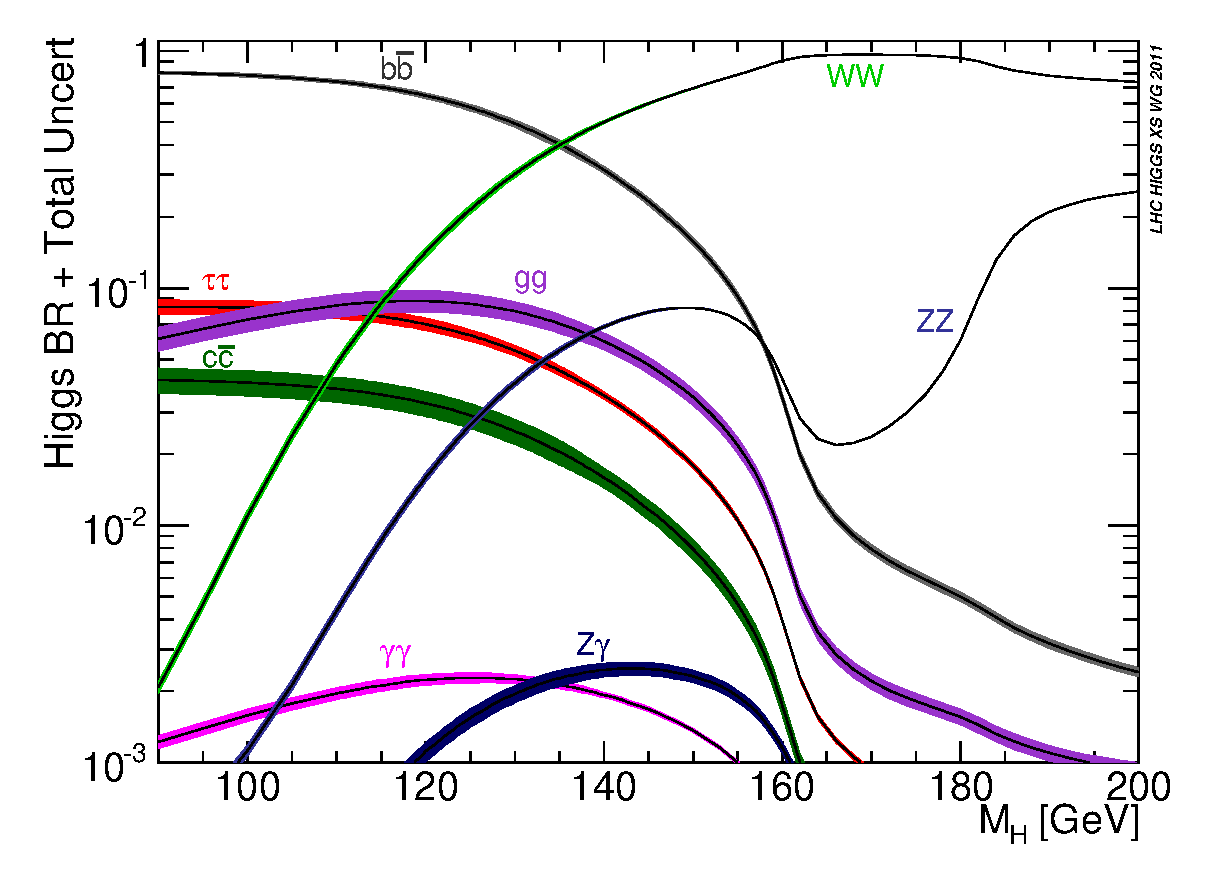
\includegraphics[width=0.6\textwidth]{htx_analysis_14ifb/figures/BRTotalUncertBands_lm}}
	\caption{Theoretical computation of Standard Model Higgs 
        branching ratios with uncertainties as a function of the 
        mass of the boson, from~\cite{Denner:2011mq}.\label{fig:HBR}}
\end{center}\end{figure}
Table~\ref{tab:htxjetmult} reports the number of jets and \btag ged jets
in the possible final states with one heavy vector-like quark decaying
to a Higgs boson and a top quark, and the other decaying in one
of the three allowed channels. It can be noticed that the lowest
\bjet s multiplicity is 2, and corresponds to very high jet multiplicities
($\geq 8$). 
The corresponding multiplicities for the main irreducible background 
contribution, \ttbar\ events produced in association with jets,
start from a baseline of 4 jets, 2 of them \btag ged, from the
$\ttbar\to W^+bW^-\bar{b}\to qqbbl\nu$, to which the associated 
jets add up. 

\begin{table}[htb]\centering
\begin{tabular}{lccccccc}\toprule
& & \multicolumn{2}{c}{$Wb$} & \multicolumn{2}{c}{$Ht$} & \multicolumn{2}{c}{$Zt$} \\\midrule
& & \#jets & \#\bjet s  & \#jets & \#\bjet s  & \#jets & \#\bjet s \\
\multirow{2}{*}{$Ht$}  & min \#\bjet s & 8 & 2 & 12 & 2 & 10 & 2\\ 
                       & max \#\bjet s & 6 & 4 & 8 & 6  & 8 & 6\\ 
\bottomrule\end{tabular}\caption{Jets and \bjet s multiplicities in 
the various possible final states when at least one heavy quark 
decays into a Higgs boson and a top quark. The table reports the
cases with the minimum and the maximum number of \btag ged jets
in the final state.\label{tab:htxjetmult}}
\end{table}


The choice is then to opt for an inclusive selection
of $\geq 6$ jets and consider three different channels
with different \btag ged jet multiplicities
in order to increase the search sensitivity.
Indeed it will be shown that even though the majority
of the signal lies in the selection with $\geq 4$ \bjet s,
the additional two channels with lower \btag ged jet multiplicities
help constraining the dominant background contributions.

Considering the higher mass of the heavy vector-like quark, compared to its
backgrounds it will transfer more momentum to its decay products.
Therefore the $\HT$ variable, 
defined as the scalar sum of the lepton transverse momentum, the missing transverse
energy \met\ and the transverse momentum of all the jets of the event:
\begin{equation}\label{eq:htxHT}
\HT = \pT(l) + \met + \sum_{j = 1}^{\rm N jets}\pT(j),
\end{equation}
is a good choice as discriminant variable to perform the statistical 
analysis on. Indeed as a consequence of its construction the $\HT$ distribution 
typically peaks at $2 m_{\T}$ and at lower values for the dominant 
$t\bar{t}$ background, as can be seen in Figure~\ref{fig:htxHTbkg}.
Furthermore this variable is rather independent of the signal decay 
mode, as shown in Figure~\ref{fig:htxHTdecays}.

\begin{figure}[h!tb]\begin{center}
	\subfigure[]{\label{fig:htxHTdecays}
  	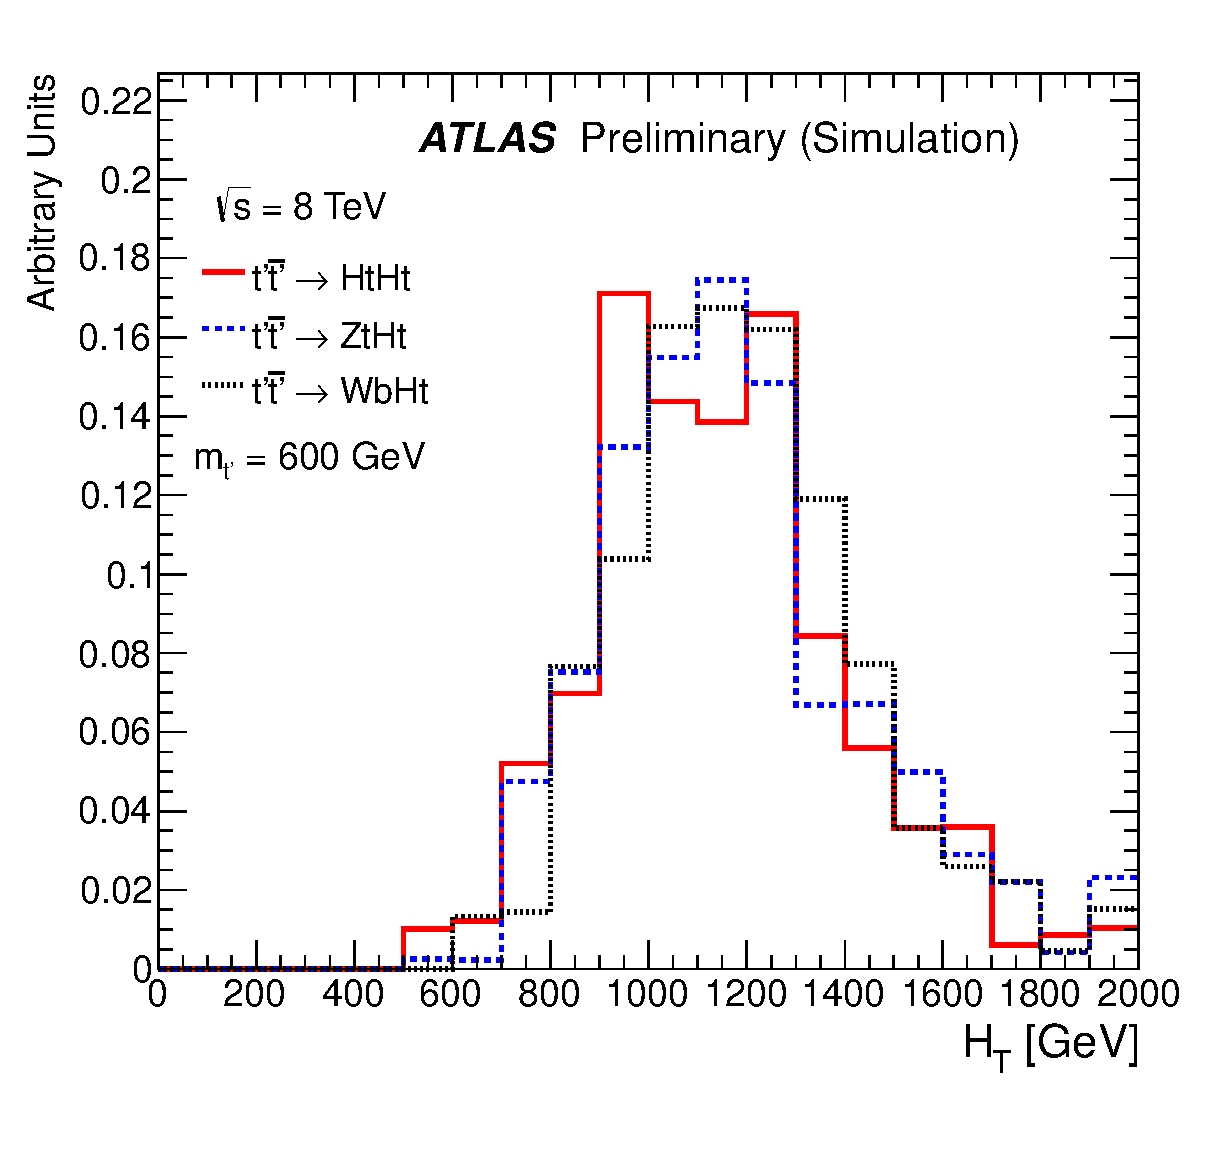
\includegraphics[width=0.45\textwidth]{htx_analysis_14ifb/figures/checks/HTAll_ELEMUON_6jetin4btagin_NOMINAL_decaysVLT}}
	\subfigure[]{\label{fig:htxHTbkg}
  	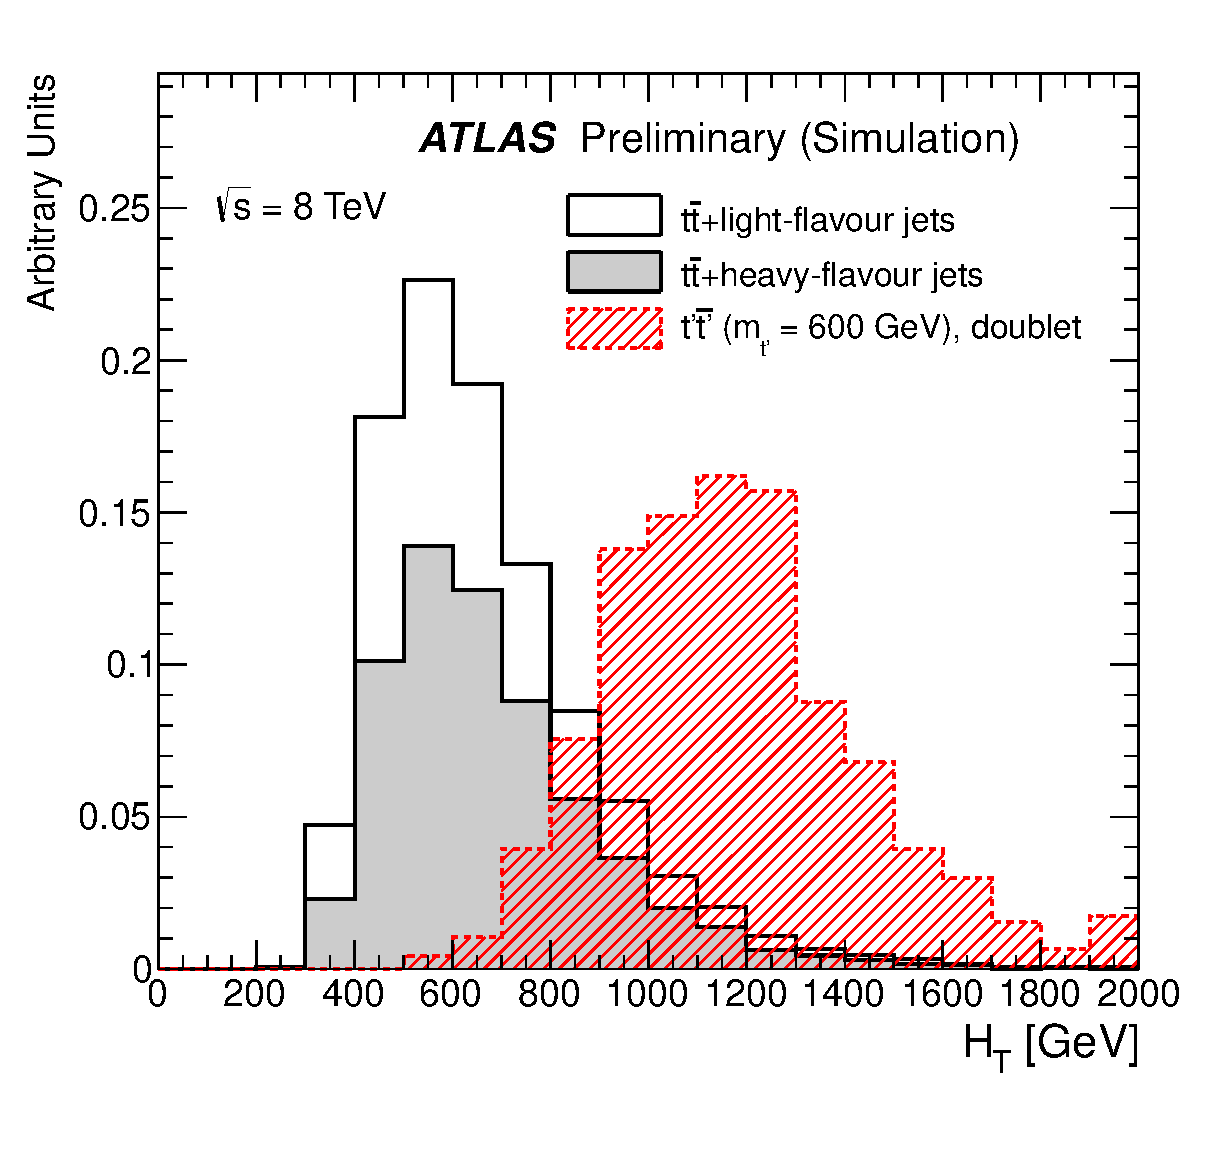
\includegraphics[width=0.45\textwidth]{htx_analysis_14ifb/figures/checks/HTAll_ELEMUON_6jetin4btagin_NOMINAL_VLTtt}}
	\caption{Comparison of the shape of the $\HT$ distribution in simulation for (a) different $\TT$ decay modes, assuming $m_{\T}=600\gev$,
and (b) between $t\bar{t}$+jets background (with $t\bar{t}$+light jets and $t\bar{t}$+heavy-flavour jets shown stacked) 
and $\TT$ signal ($m_{\T}=600\gev$) in the $\T$ doublet scenario.
The selection used corresponds to the combined electron and muon channels with $\geq 6$ jets and $\geq 4$ $b$ tags. 
The last bin in all figures contains the overflow.}
\end{center}\end{figure}

To model the \ttbar\ background
the \texttt{ALPGEN} Monte Carlo generator is chosen, which well
describes high jet multiplicity regions and allows the separation
between the heavy-flavor (``\ttbar+HF'') and the light-flavor
(``\ttbar+light'') components of these events.
Figure~\ref{fig:HT_checks_ttjetsComp} shows a slightly harder
$\HT$ distribution for the \tthf\ background compared to the
\ttlf\ one.

\begin{figure}[h!tb]\begin{center}
	\subfigure[]{
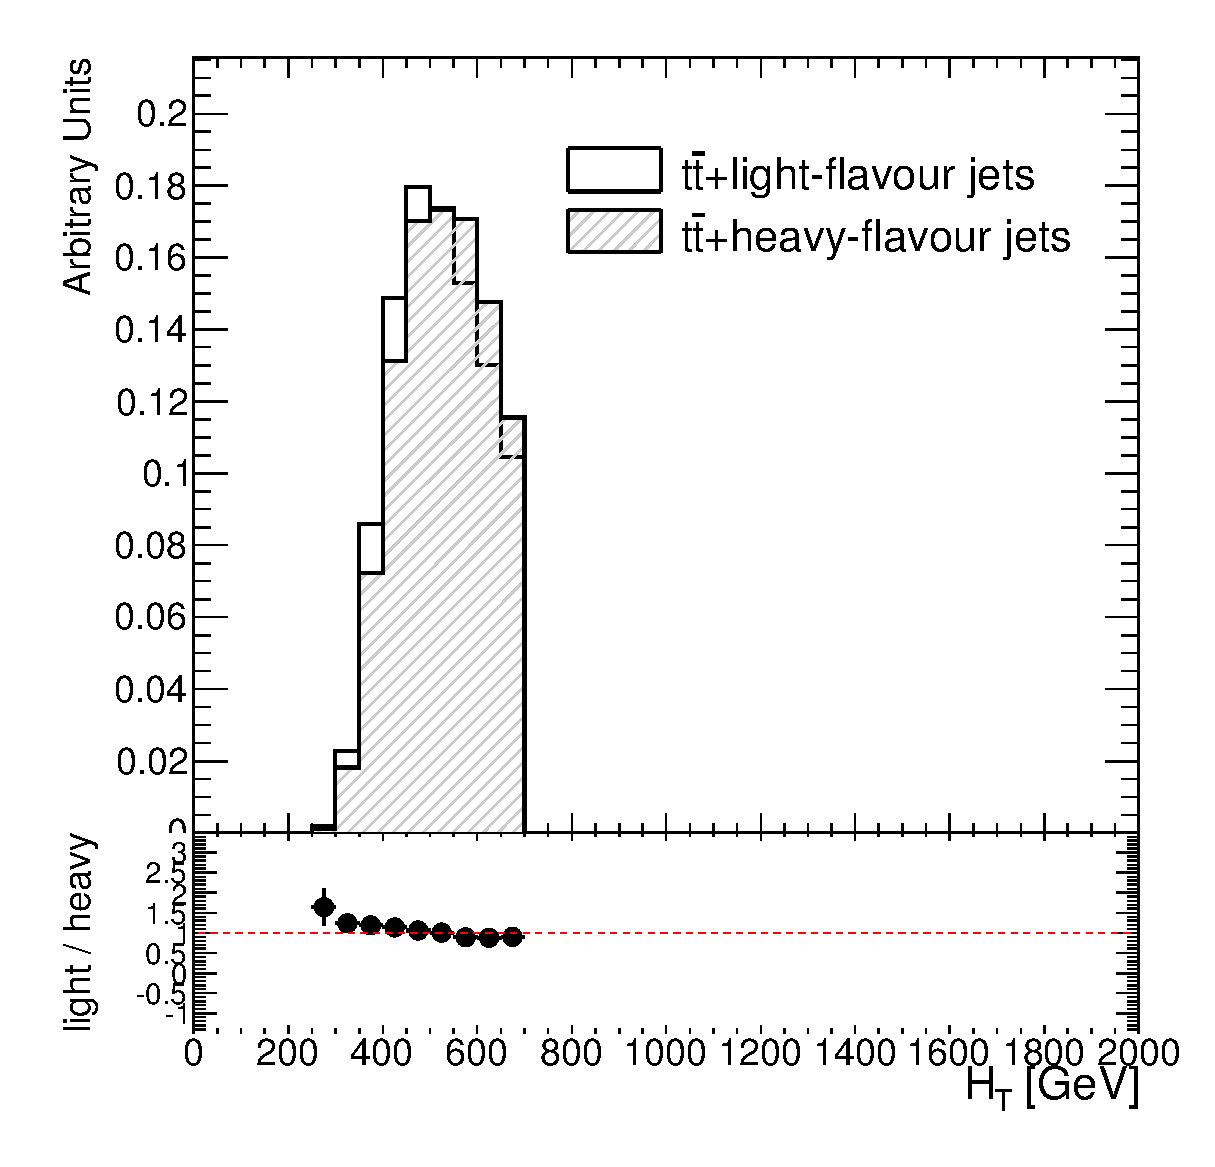
\includegraphics[width=0.3\textwidth]{htx_analysis_14ifb/figures/checks/ttcomp_HTAll_ELEMUON_6jetin2btagex_NOMINAL_mod.eps}}
	\subfigure[]{
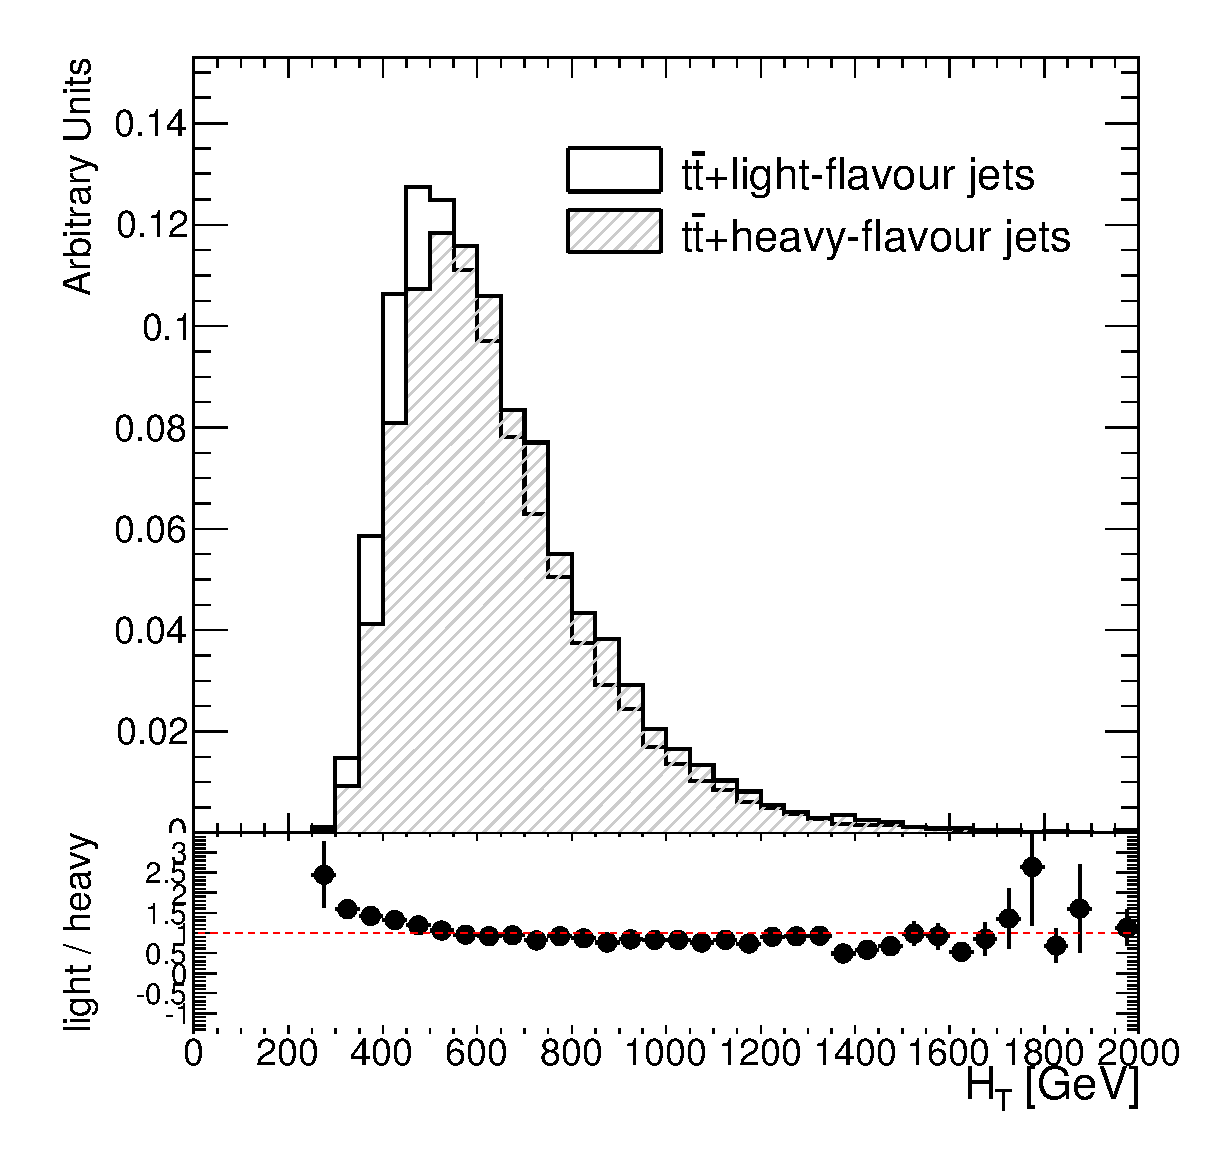
\includegraphics[width=0.3\textwidth]{htx_analysis_14ifb/figures/checks/ttcomp_HTAll_ELEMUON_6jetin3btagex_NOMINAL_mod.eps}}
	\subfigure[]{
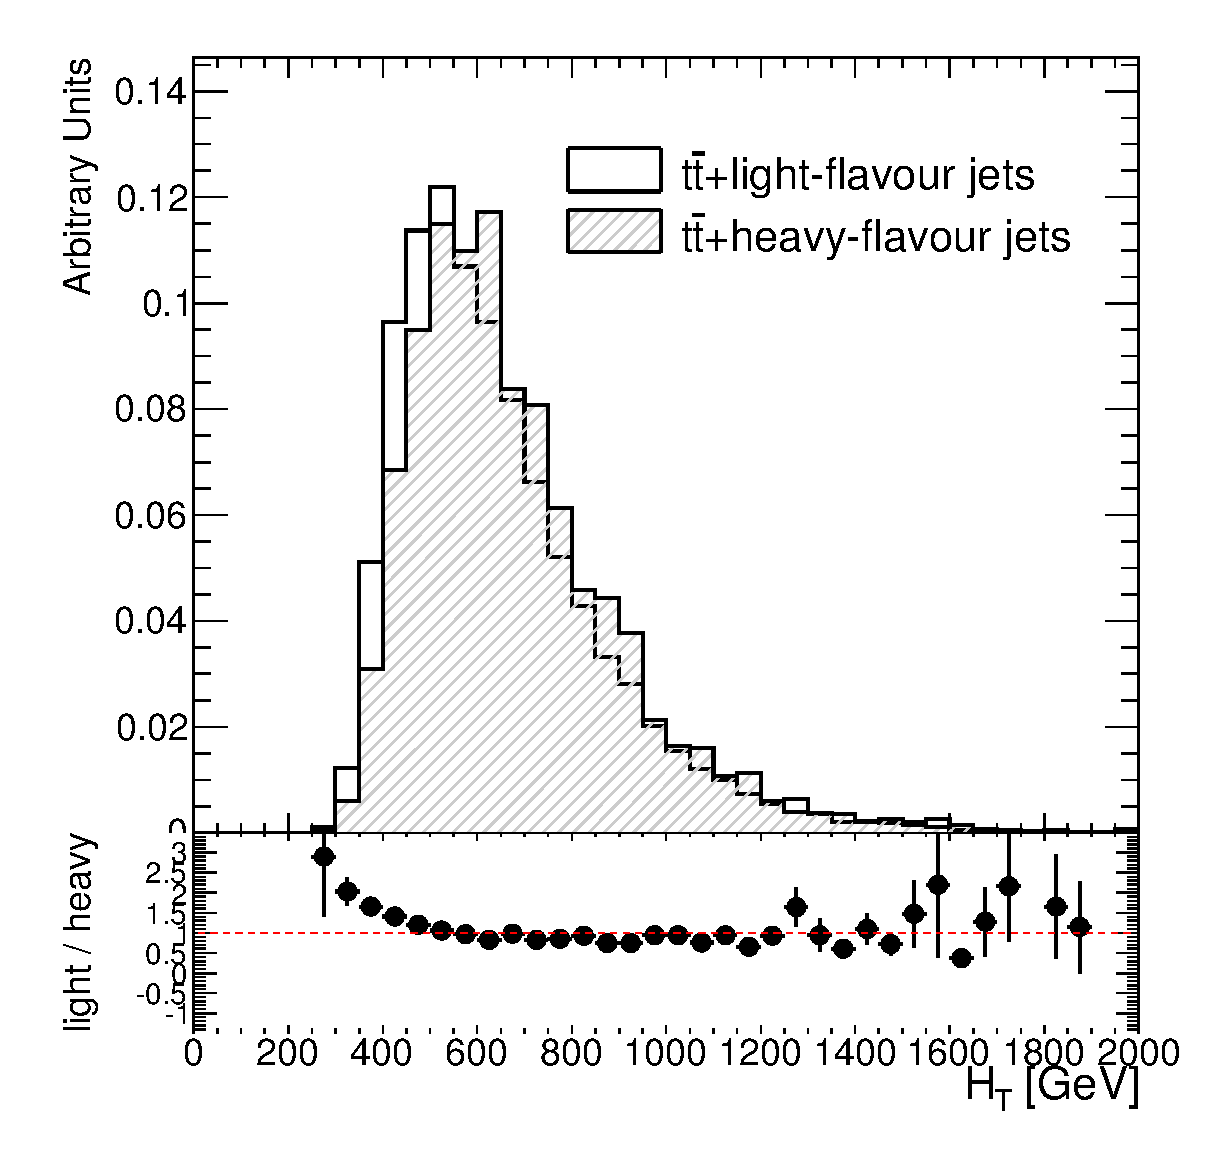
\includegraphics[width=0.3\textwidth]{htx_analysis_14ifb/figures/checks/ttcomp_HTAll_ELEMUON_6jetin4btagin_NOMINAL_mod.eps}}
	\caption{Comparison of the shape of the $\HT$ distribution in simulation between the $t\bar{t}$+light jets and $t\bar{t}$+heavy-flavour jets backgrounds.
The selection used corresponds to the combined electron and muon channels with $\geq 6$ jets and (a) 2 $b$ tags, 
(b) 3 $b$-tags and (c) $\geq 4$ $b$ tags. The last bin in all figures contains the overflow.\label{fig:HT_checks_ttjetsComp}}
\end{center}\end{figure}




\section{Event selection}\label{sec:htxEVT}

Following the general ideas developed in Section~\ref{sec:htxMULT}, the
natural choice to further optimize the preselection cuts presented in 
Section~\ref{sec:presel} is to require higher jets and \bjet s multiplicities.
The lowest number of jets in the final state comes from the $\TTbar\to HtW^-\bar{b}$
channel and amounts to 6 jets. Therefore, in the final selection at least 6 jets
(with the same characteristics explained in Section~\ref{sec:htxMULT}) are required.
Then, in order to maximize the signal acceptance, considering the fact that the
\btag ging efficiency is not 100\%, at least 2 of these jets are
required to be \btag ged.
We remind here that in the \wbx\ analysis an orthogonality
cut is applied, rejecting events that have $\geq 6$ jets and $\geq 3$
\btag ged jets. This would still cause an overlap of the two analyses
in the case of 2 \btag ged jets, and therefore in the \htx\ analysis
a cut on the $H_T$ variable opposite to the one required in the 
signal regions of the \wbx\ analysis is applied. 
Since the definition of the $H_T$ variable is slightly different 
in the two analyses, the cut applied results conservative.

As was already hinted in Section~\ref{sec:trf}, 
applying direct cuts on the events based on the number of \btag ged jets
can result in a dramatic reduction of statistic population of the Monte
Carlo simulated samples. To overcome this problem the Tag Rate Function
method is used for all the Monte Carlo background samples. Details on
the method and on the validation checks can be found in Appendix~\ref{app:trf}.

The final selection is further splitted in different \bjet\ multiplicity 
channels in order to optimize the search sensitivity, as it can be
easily understood that the higher the number of \btag ged jets are
identified, the less background contamination, 
the better $S/B$ ratio is obtained. Three channels are
defined as follows: the \chii\ channel, with exactly two \btag ged jets;
the \chiii\ channel, with exactly three \btag ged jets;
the \chiv\ channel, with at least four \btag ged jets.
In order to ensure orthogonality with the \wbx\ analysis
in the \chii\ channel, the choice was done to blind this channel
from signal and maintain it to exploit the high contamination from
\ttbar\ background contribution in the containment of systematic
uncertainties. The blinding cut applied relies on the $\HT$ variable,
which was defined in Equation~\ref{eq:htxHT}.
The \HT\ variable definition differs from the \htfj\ one of the \wbx\ analysis,
where the scalar sum over the jets' transverse momenta run only
over the four leading jets. In the \wbx\ analysis signal region the 
events were selected with $\htfj > 800~\gev$. In the \htx\ 
analysis events in the \chii\ channel with $\HT > 700~\gev$
are rejected. This cut is somehow over-conservative, as $\HT>\htfj$
and the lower threshold of 700~\gev\ was actually chosen with in mind
the previous search for fourth generation top quarks performed with
ATLAS data from pp collisions at a \cme\ of 7~\tev~\cite{ATLAS:2012qe}.
Table~\ref{tab:htxselection} summarises the cuts applied in the event selection,
while Table~\ref{tab:Yields_blind} shows the final expected and
observed number of events in the three channels, after applying 
the blinding cut $\HT < 700~\gev$.

\begin{table}[tb]
\begin{center}
\begin{tabular}{ll}
\toprule
Selection & Requirements \\
\midrule
Preselection & One electron or muon  \\
             & $\met >20\gev$, $\met +m_{\rm T}>60\gev$ \\
             & $\geq 4$ jets, $\geq 1$ $b$-tagged jets \\
\midrule
\chii\ selection & $\geq 6$ jets, =2 $b$-tagged jets \\
 & orthogonality cut: \\
 & $\HT < 700~\gev$ \\
\midrule
\chiii\ selection & $\geq 6$ jets,  =3 $b$-tagged jets \\
\midrule
\chiv\ selection &$\geq 6$ jets,  $\geq 4$ $b$-tagged jets \\
\bottomrule
\end{tabular}
\caption{Summary of event selection requirements.}
\label{tab:htxselection}
\end{center}
\end{table}

\begin{table}[tb]\centering
\begin{tabular}{l D{;}{\,\pm\,}{-1} D{;}{\,\pm\,}{-1} D{;}{\,\pm\,}{-1} } \toprule\toprule
 & \multicolumn{1}{c}{ $\geq 6$ jets, $= 2$ $b$-tags } 		 & \multicolumn{1}{c}{ $\geq 6$ jets, $= 3$ $b$-tags } 		 & \multicolumn{1}{c}{ $\geq 6$ jets, $\geq 4$ $b$-tags } 		 \\ \midrule 
  MultiJet  & 49;11  & 1;0  & 0;0 \\ 
 Single top  & 300;10  & 47;3  & 4;1 \\ 
 Diboson  & 2;0  & 0;0  & 0;0 \\ 
 $Z$+jets  & 50;6  & 4;1  & 0;0 \\ 
 $W$+jets  & 249;20  & 34;6  & 3;1 \\ 
 $t\bar{t}$V  & 71;0  & 19;0  & 3;0 \\ 
 $t\bar{t}$H (125)  & 28;0  & 17;0  & 6;0 \\ 
 $t\bar{t}$+HF  & 1222;12  & 486;6  & 86;2 \\ 
 $t\bar{t}$+light  & 10811;38  & 1534;7  & 58;1 \\ 
\midrule 
  Tot Bkg w/ Alpgen  & 12783;48  & 2142;11  & 160;2 \\ \midrule 
  $T\bar{T}$ (600) doublet  & 4;0  & 3;0  & 1;0 \\ 
 Data  & 11885;109  & 2061;45  & 222;15 \\ 
\bottomrule\end{tabular}
\caption{Predicted and observed yields in the combined 
electron and muon \chii, \chiii\ and \chiv\ channels
blinded using the cut $\HT<700~\gev$. 
Also shown is the expected $\TT$ signal in both the doublet 
and singlet scenarios for $m_{\T}=600~\gev$. 
The uncertainties shown 
are 
statistical only.
\label{tab:Yields_blind}}
\end{table}


The acceptance  times efficiency for the \chii, \chiii\ and 
\chiv\ selections are given respectively in 
Tables~\ref{tab:eff_ch2},~\ref{tab:eff_ch3} and~\ref{tab:eff_ch4}
separately for each of the allowed \TTbar\ decay modes that can enter
the selections and as a function of $m_{\T}$.
From these numbers it is evident that the \chii\ channel is
poorly sensitive to any \T\ decay mode, as expected,
while the \chiii\ channel helps to increase the acceptance
for the decay modes with at least one $\T\to Wb$ and 
for $\TTbar \to ZtZt$.
\begin{table}[h!tb]
\begin{center}%\footnotesize
\begin{tabular}{c c c c c c c c c c c } \toprule
 & \multicolumn{6}{c}{ Decay mode } \\
 $m_{T}$ (GeV)  & WbWb 		 & WbZt 		 & WbHt 		 & ZtHt 		 & HtHt 		 & ZtZt 		 \\ \midrule 
 350 & 0.41\% & 1.18\% & 1.42\% & 2.18\% & 2.22\% & 1.79\%\\ 
400 & 0.22\% & 0.69\% & 0.95\% & 1.53\% & 1.87\% & 1.19\%\\ 
450 & 0.14\% & 0.36\% & 0.52\% & 0.91\% & 0.99\% & 0.71\%\\ 
500 & 0.10\% & 0.20\% & 0.26\% & 0.52\% & 0.63\% & 0.38\%\\ 
550 & 0.03\% & 0.12\% & 0.17\% & 0.30\% & 0.31\% & 0.30\%\\ 
600 & 0.03\% & 0.07\% & 0.08\% & 0.18\% & 0.18\% & 0.11\%\\ 
650 & 0.01\% & 0.04\% & 0.09\% & 0.11\% & 0.09\% & 0.10\%\\ 
700 & 0.01\% & 0.03\% & 0.03\% & 0.06\% & 0.09\% & 0.05\%\\ 
750 & 0.01\% & 0.02\% & 0.03\% & 0.05\% & 0.05\% & 0.05\%\\ 
800 & 0.01\% & 0.01\% & 0.01\% & 0.02\% & 0.05\% & 0.03\%\\ 
\bottomrule\end{tabular}
\caption{Acceptance times efficiency for different \TTbar\ decay modes as a function of $m_{\T}$ for the \chii\ selection.}
\label{tab:eff_ch2}
\end{center}
%\end{table}
%\begin{table}
\begin{center}%\footnotesize
\begin{tabular}{c c c c c c c c c c c } \toprule
 & \multicolumn{6}{c}{ Decay mode } \\
 $m_{T}$ (GeV)  & WbWb 		 & WbZt 		 & WbHt 		 & ZtHt 		 & HtHt 		 & ZtZt 		 \\ \midrule 
 350 & 0.45\% & 1.11\% & 2.31\% & 2.71\% & 3.57\% & 1.68\%\\ 
400 & 0.40\% & 1.23\% & 2.65\% & 3.15\% & 4.22\% & 1.83\%\\ 
450 & 0.48\% & 1.47\% & 2.90\% & 3.32\% & 4.42\% & 2.01\%\\ 
500 & 0.52\% & 1.50\% & 3.00\% & 3.60\% & 4.45\% & 2.11\%\\ 
550 & 0.61\% & 1.41\% & 3.10\% & 3.67\% & 4.40\% & 2.17\%\\ 
600 & 0.53\% & 1.63\% & 3.34\% & 3.71\% & 4.47\% & 2.30\%\\ 
650 & 0.58\% & 1.47\% & 3.09\% & 3.70\% & 4.71\% & 1.99\%\\ 
700 & 0.48\% & 1.38\% & 3.22\% & 3.54\% & 4.55\% & 2.15\%\\ 
750 & 0.52\% & 1.44\% & 3.08\% & 3.61\% & 4.46\% & 2.16\%\\ 
800 & 0.53\% & 1.41\% & 3.09\% & 3.43\% & 4.29\% & 2.10\%\\ 
\bottomrule\end{tabular}
\caption{Acceptance times efficiency for different \TTbar\ decay modes as a function of $m_{\T}$ for the \chiii\ selection.}
\label{tab:eff_ch3}
\end{center}
%\end{table}
%\begin{table}
\begin{center}%\footnotesize
\begin{tabular}{c c c c c c c c c c c } \toprule
 & \multicolumn{6}{c}{ Decay mode } \\
 $m_{T}$ (GeV)  & WbWb 		 & WbZt 		 & WbHt 		 & ZtHt 		 & HtHt 		 & ZtZt 		 \\ \midrule 
 350 & 0.06\% & 0.31\% & 1.00\% & 1.56\% & 3.07\% & 0.69\%\\ 
400 & 0.06\% & 0.39\% & 1.19\% & 1.95\% & 3.53\% & 0.80\%\\ 
450 & 0.04\% & 0.44\% & 1.43\% & 2.13\% & 4.20\% & 0.95\%\\ 
500 & 0.08\% & 0.51\% & 1.59\% & 2.38\% & 4.48\% & 0.99\%\\ 
550 & 0.05\% & 0.55\% & 1.56\% & 2.37\% & 4.80\% & 0.92\%\\ 
600 & 0.05\% & 0.54\% & 1.78\% & 2.69\% & 5.08\% & 1.10\%\\ 
650 & 0.08\% & 0.52\% & 1.67\% & 2.49\% & 4.96\% & 1.04\%\\ 
700 & 0.06\% & 0.53\% & 1.69\% & 2.55\% & 4.97\% & 1.00\%\\ 
750 & 0.05\% & 0.42\% & 1.73\% & 2.62\% & 4.90\% & 1.15\%\\ 
800 & 0.07\% & 0.50\% & 1.72\% & 2.48\% & 4.90\% & 1.05\%\\ 
\bottomrule\end{tabular}
\caption{Acceptance times efficiency for different \TTbar\ decay modes as a function of $m_{\T}$ for the \chiv\ selection.}
\label{tab:eff_ch4}
\end{center}
\end{table}
Since this search is optimized for the
$\T \to Ht$ decay mode of the heavy quark (as can be seen in
Table~\ref{tab:eff_ch4}), the theoretical
scenario to which it is mostly sensitive is the doublet
model, \TB\ or \XT,
where the mass-dependent branching ratio of $\T \to Ht$ is
significantly higher than the others (as was shown in Figure~\ref{fig:vlqBRs}).
As explained in Section~\ref{sec:MCbkg}, the Monte Carlo signal samples
are simulated for singlet \T\ with branching ratio of 1/3 for
every decay mode and then reweighted at analysis level to obtain the
branching ratios of the desired models. 
Considering that the mixing between the singlet $\T$ quark and Standard 
Model quarks is left-handed, while for a doublet \T\ is right-handed,
a check was performed to make sure the kinematics (and thus the signal acceptance and shape
of the $\HT$ distribution)
involved in the search is not affected.
Two Monte Carlo samples for the doublet scenario, 
corresponding to $m_{\T}=350$ and $600\gev$, were available and
have been used in this study. 
Figure~\ref{fig:HT_checks_SingletvsDoubletComp} compares, for both mass
points and each of the three analysis channels considered, the yield 
and shape of the $\HT$ distribution for the 
predicted signal using the singlet and doublet samples. 
In both cases the samples were reweighted to reproduce
the branching ratios corresponding to the doublet model. 
As it can be appreciated, the shapes of the distributions
are in reasonable agreement and discrepancies in the yields 
are below 5\% in the highest-sensitivity channel (\chiv).

%%%%%%%%%%%%%%
\begin{figure}[htbp]
\begin{center}
\subfigure[]{\label{fig:singletdoublet_2b}
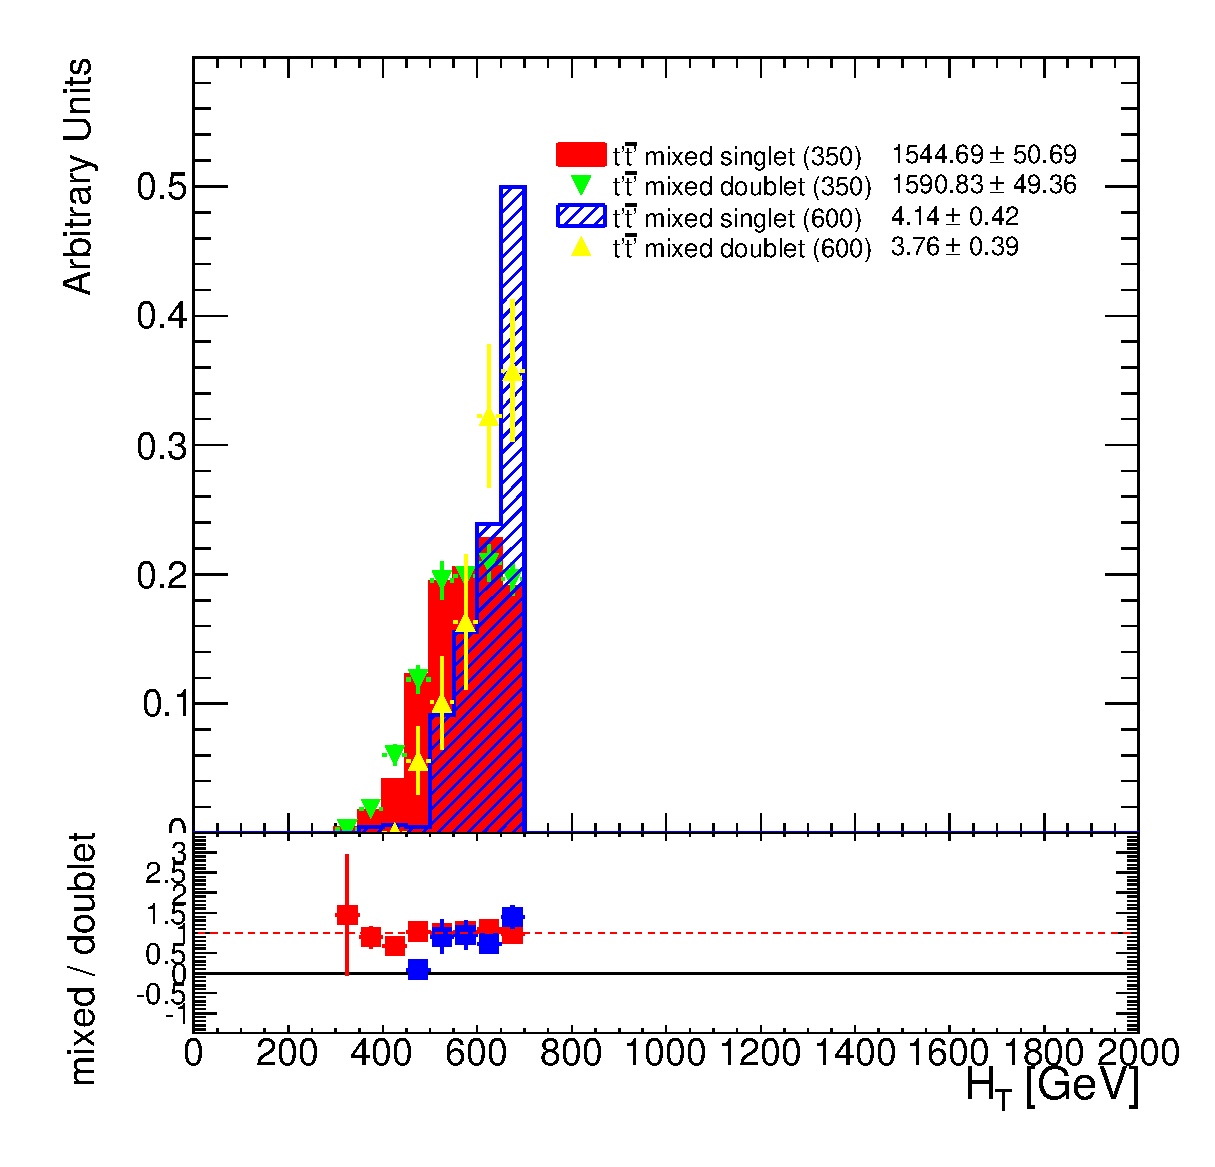
\includegraphics[width=0.32\textwidth]{htx_analysis_14ifb/figures/doubletcomp_HTAll_ELEMUON_6jetin2btagex_NOMINAL.eps}}
\subfigure[]{\label{fig:singletdoublet_3b}
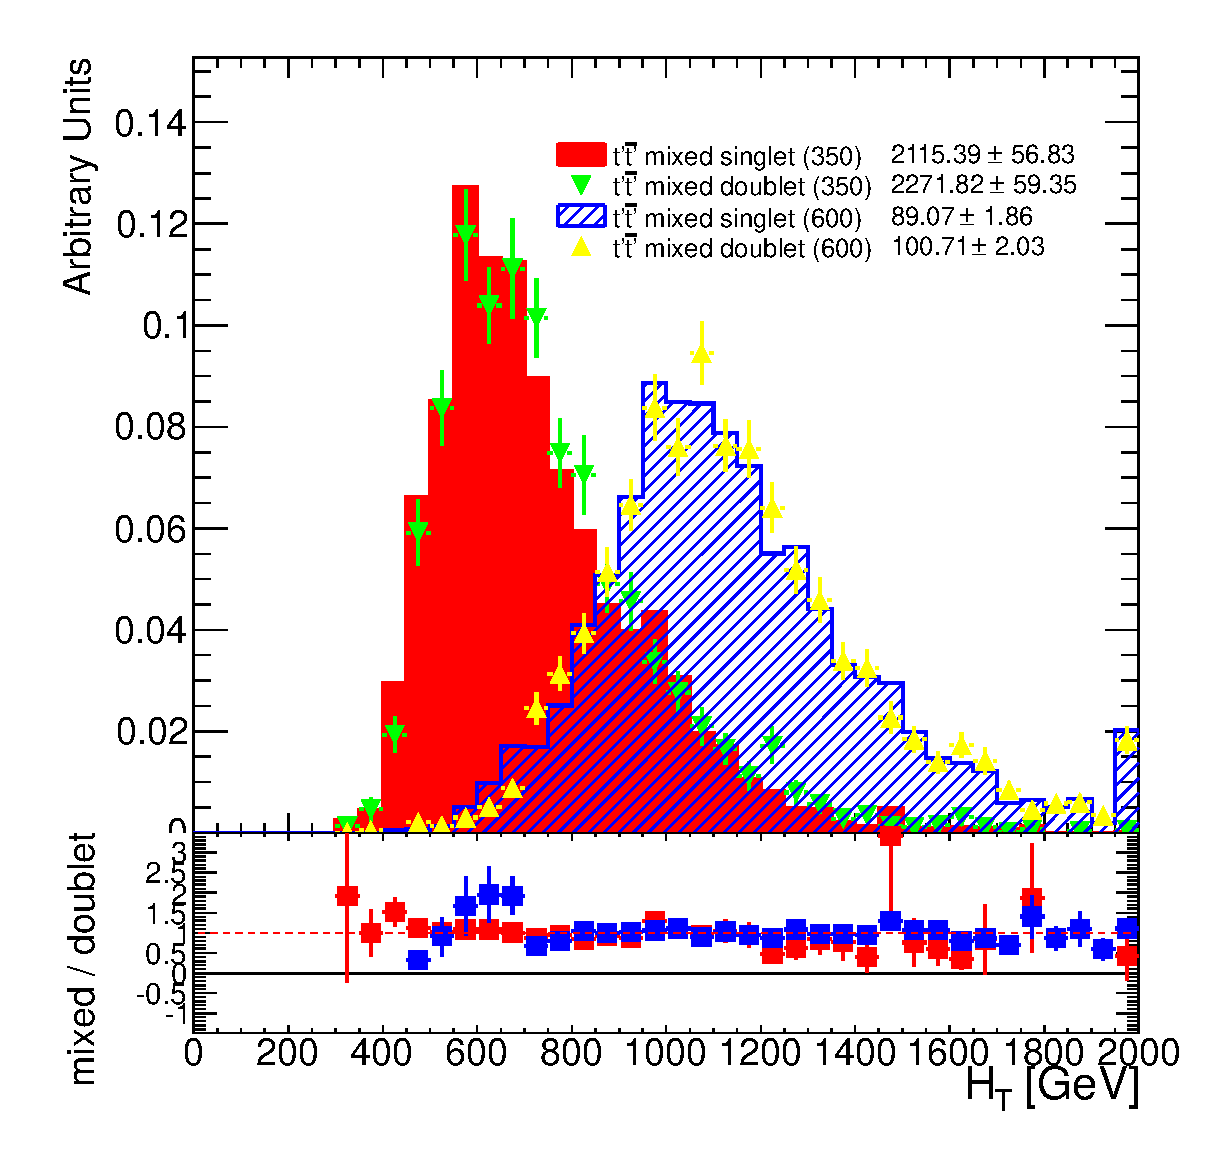
\includegraphics[width=0.32\textwidth]{htx_analysis_14ifb/figures/doubletcomp_HTAll_ELEMUON_6jetin3btagex_NOMINAL.eps}}
\subfigure[]{\label{fig:singletdoublet_4b}
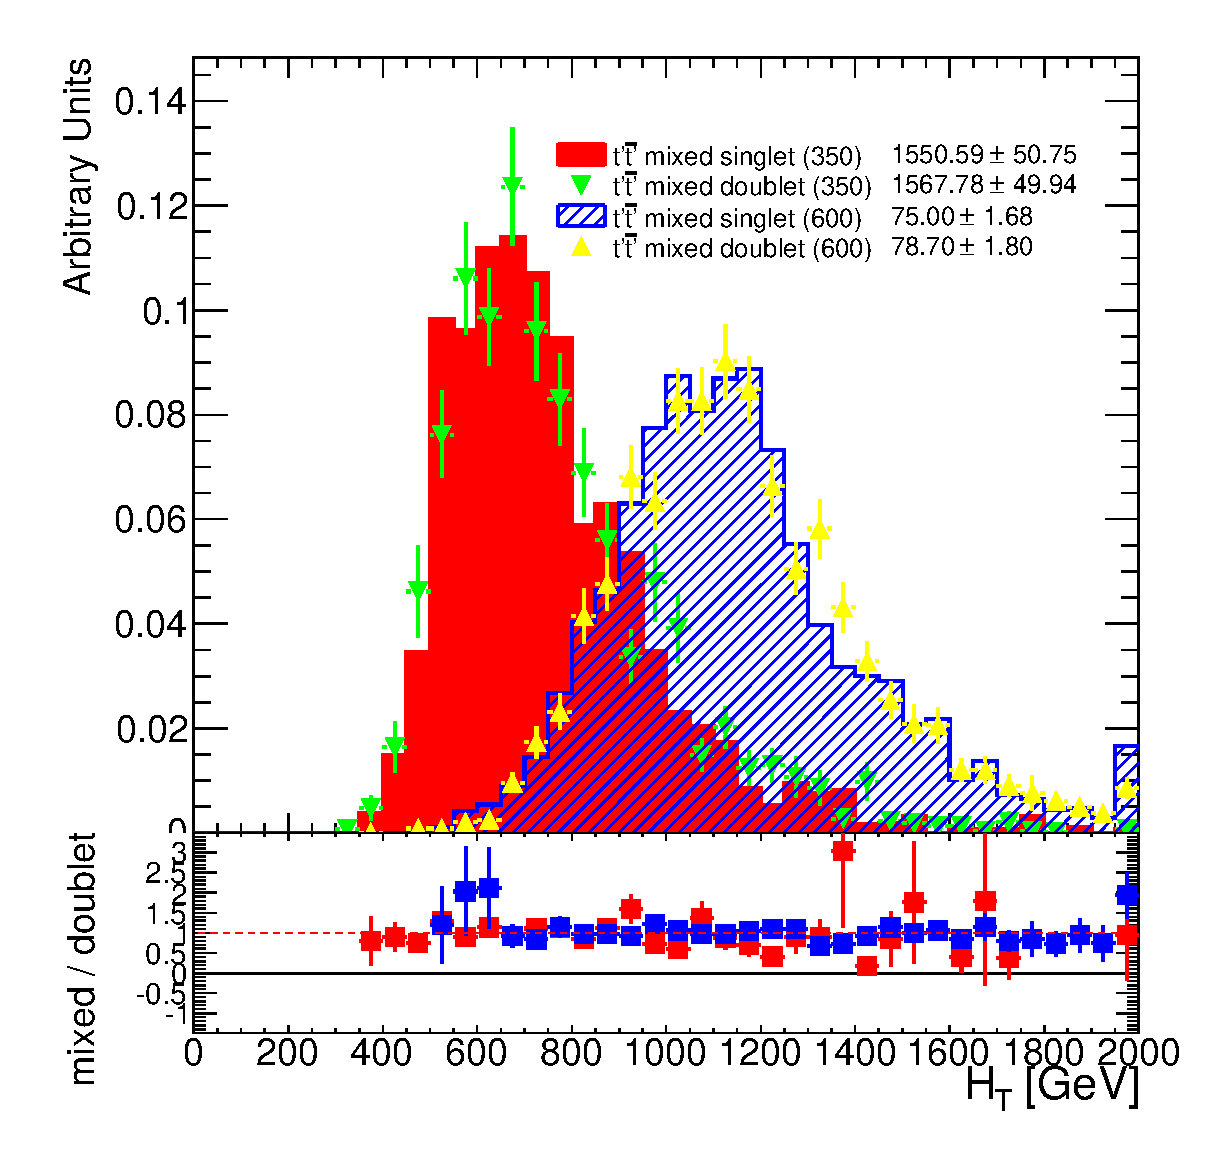
\includegraphics[width=0.32\textwidth]{htx_analysis_14ifb/figures/doubletcomp_HTAll_ELEMUON_6jetin4btagin_NOMINAL.eps}}
\caption{
Comparison of the yields and shape of the $\HT$ distribution in simulation for 
$\T$ signal using the singlet samples (points) and
using the doublet samples (full histograms). In both 
cases the signal has been reweighted to reproduce the 
branching ratios corresponding 
to the doublet model. The selection used corresponds 
to the combined electron and muon channels
with $\geq 6$ jets and (a) 2 $b$ tags,  (b) 3 $b$-tags 
and (c) $\geq 4$ $b$ tags. The comparison is made for two 
different mass points, $m_{\T}=350$ and $600\gev$.
The last bin in all figures contains the overflow.
\label{fig:HT_checks_SingletvsDoubletComp}}
\end{center}
\end{figure}



\section{Control regions}\label{sec:htxCR}

In order to assess the good modeling of the background contributions
simulated with Monte Carlo generators, dedicated ``control regions''
depleted of signal are defined. The preselection region already provides
useful control regions where the signal presence is vetoed by applying the
same blinding cut used for the \chii\ channel: $\HT < 700~\gev$.
The preselection is splitted in various control regions with different
jet and \bjet s multiplicities. Appendix~\ref{app:htxcontrol} reports
the outcome of these checks in the electron and muon channels separately
and combined. While low \bjet\ multiplicity selections show rather good
agreement between data and Standard Model backrounds (Figures~\ref{fig:unscaled2}
and~\ref{fig:unscaled3}), it is observed that
in the control region corresponding to the blinded \chiv\ channel
the background prediction appears systematically below the data 
(Figure~\ref{fig:unscaled4}).

\begin{figure}[h!tb]\begin{center}
	\subfigure[]{\label{fig:unscaled2}
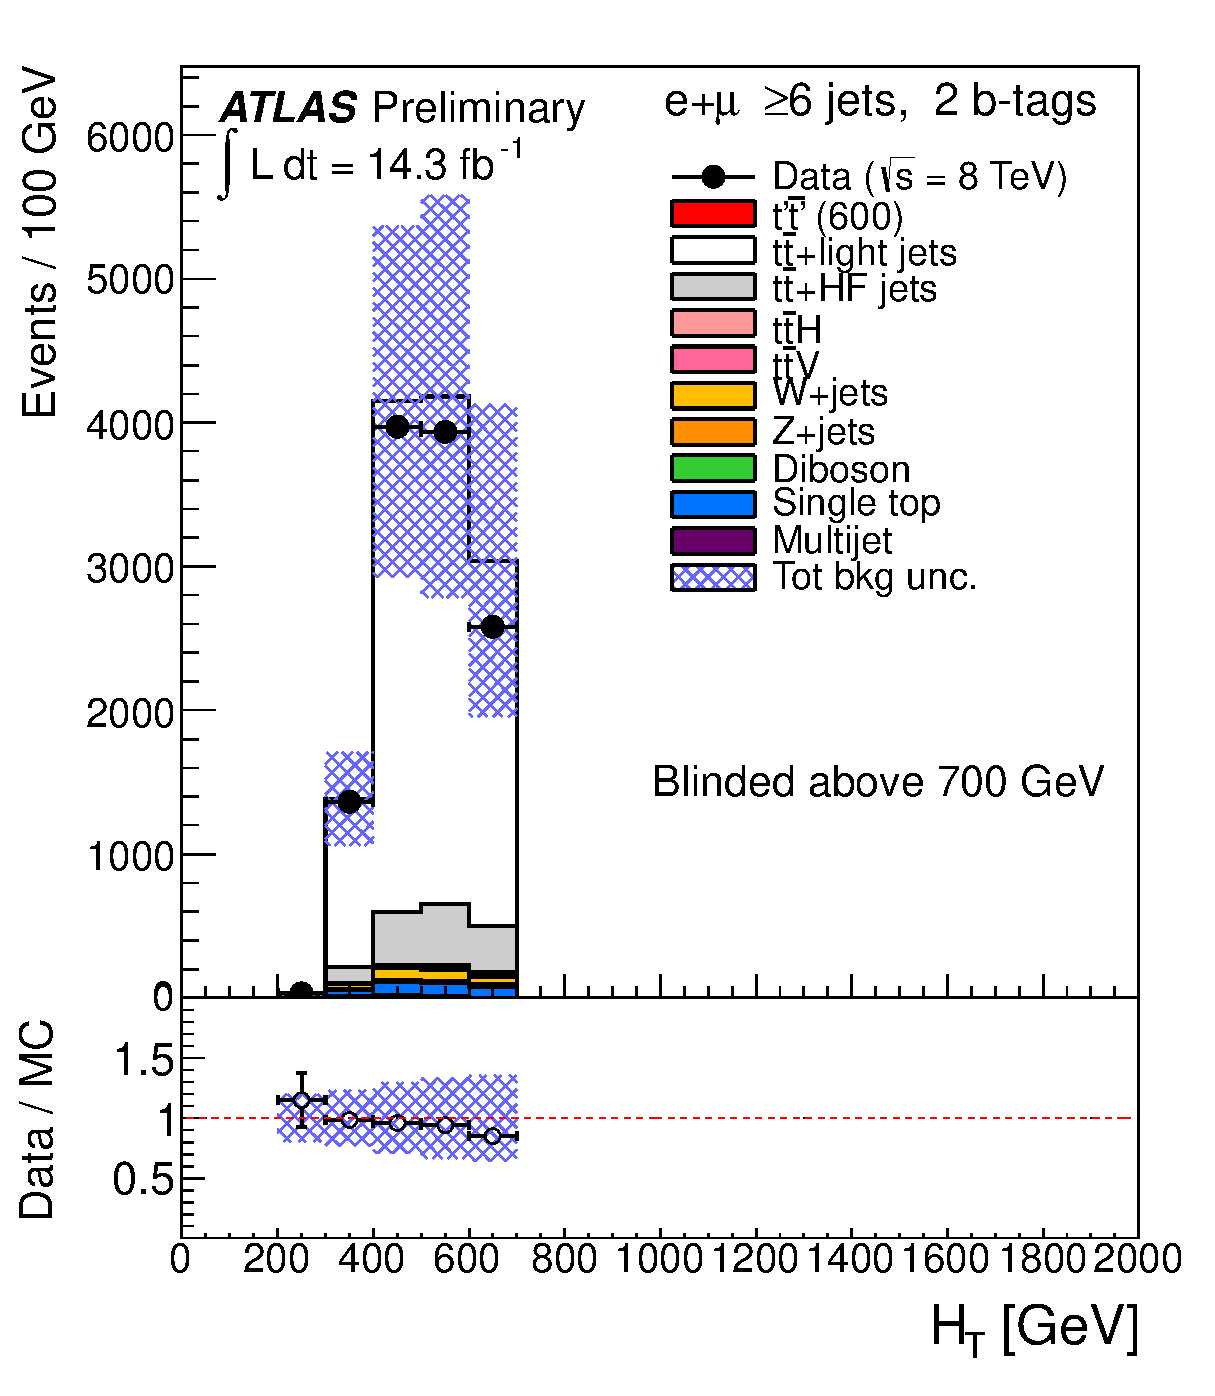
\includegraphics[width=0.3\textwidth]{htx_analysis_14ifb/figures/unscaled/HTAll_ELEMUON_6jetin2btagex_NOMINAL.eps}}
	\subfigure[]{\label{fig:unscaled3}
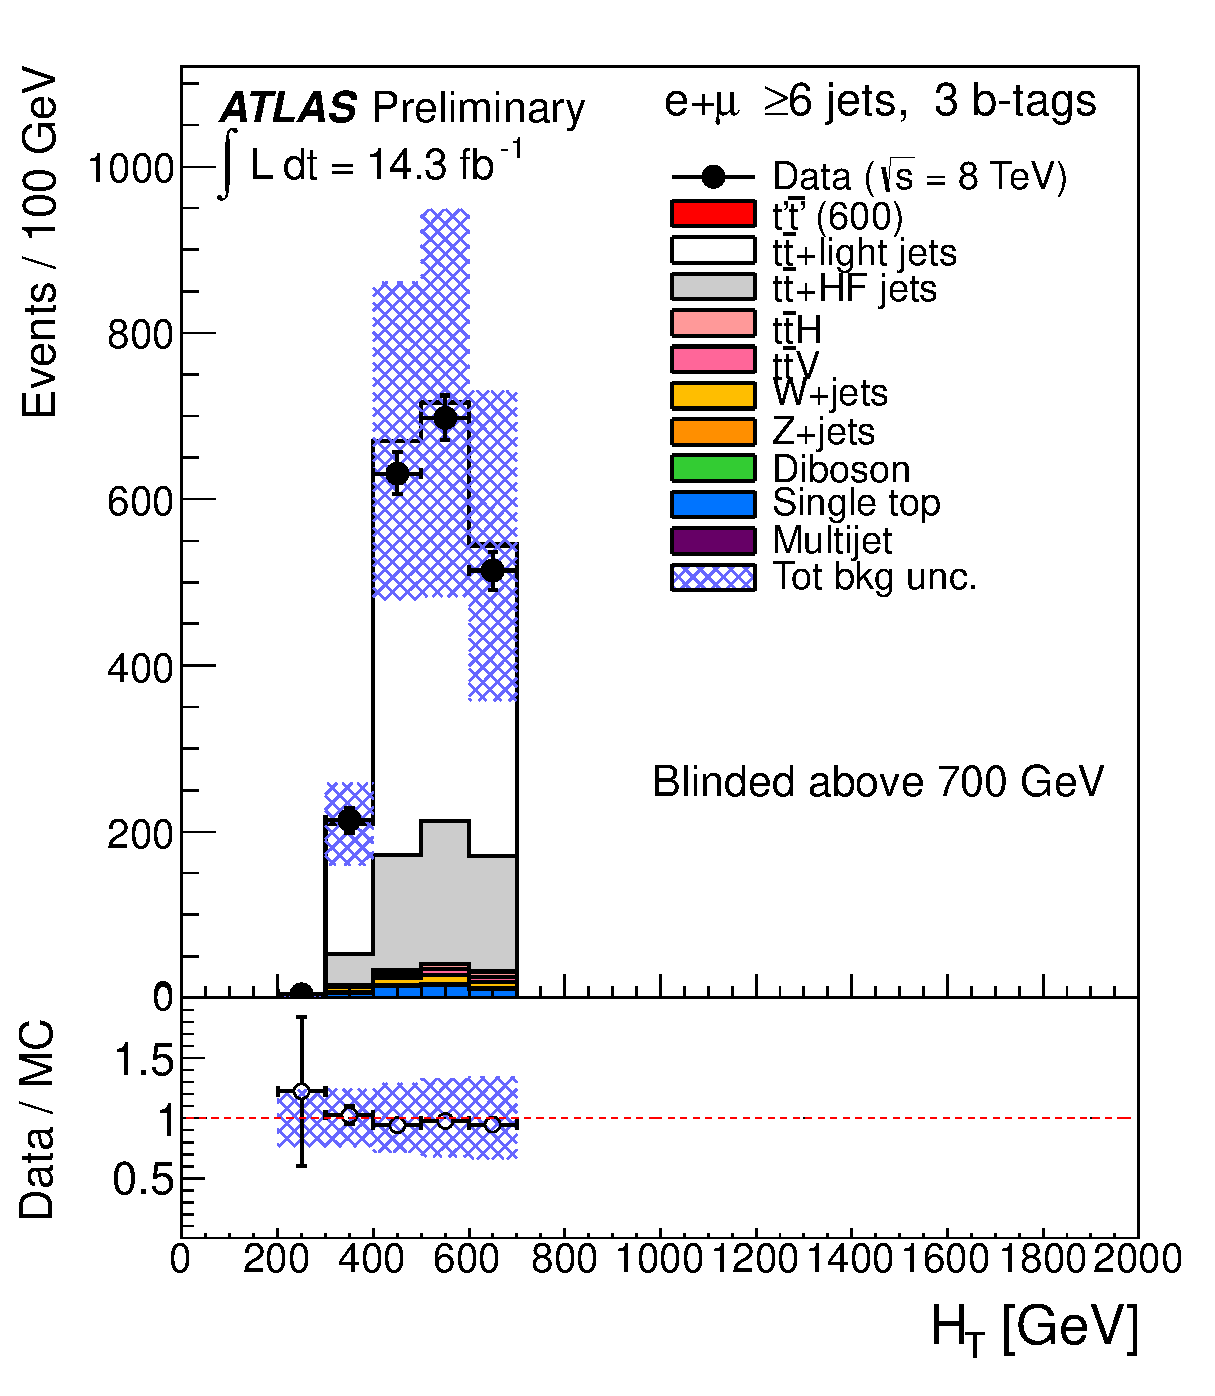
\includegraphics[width=0.3\textwidth]{htx_analysis_14ifb/figures/unscaled/HTAll_ELEMUON_6jetin3btagex_NOMINAL.eps}}
	\subfigure[]{\label{fig:unscaled4}
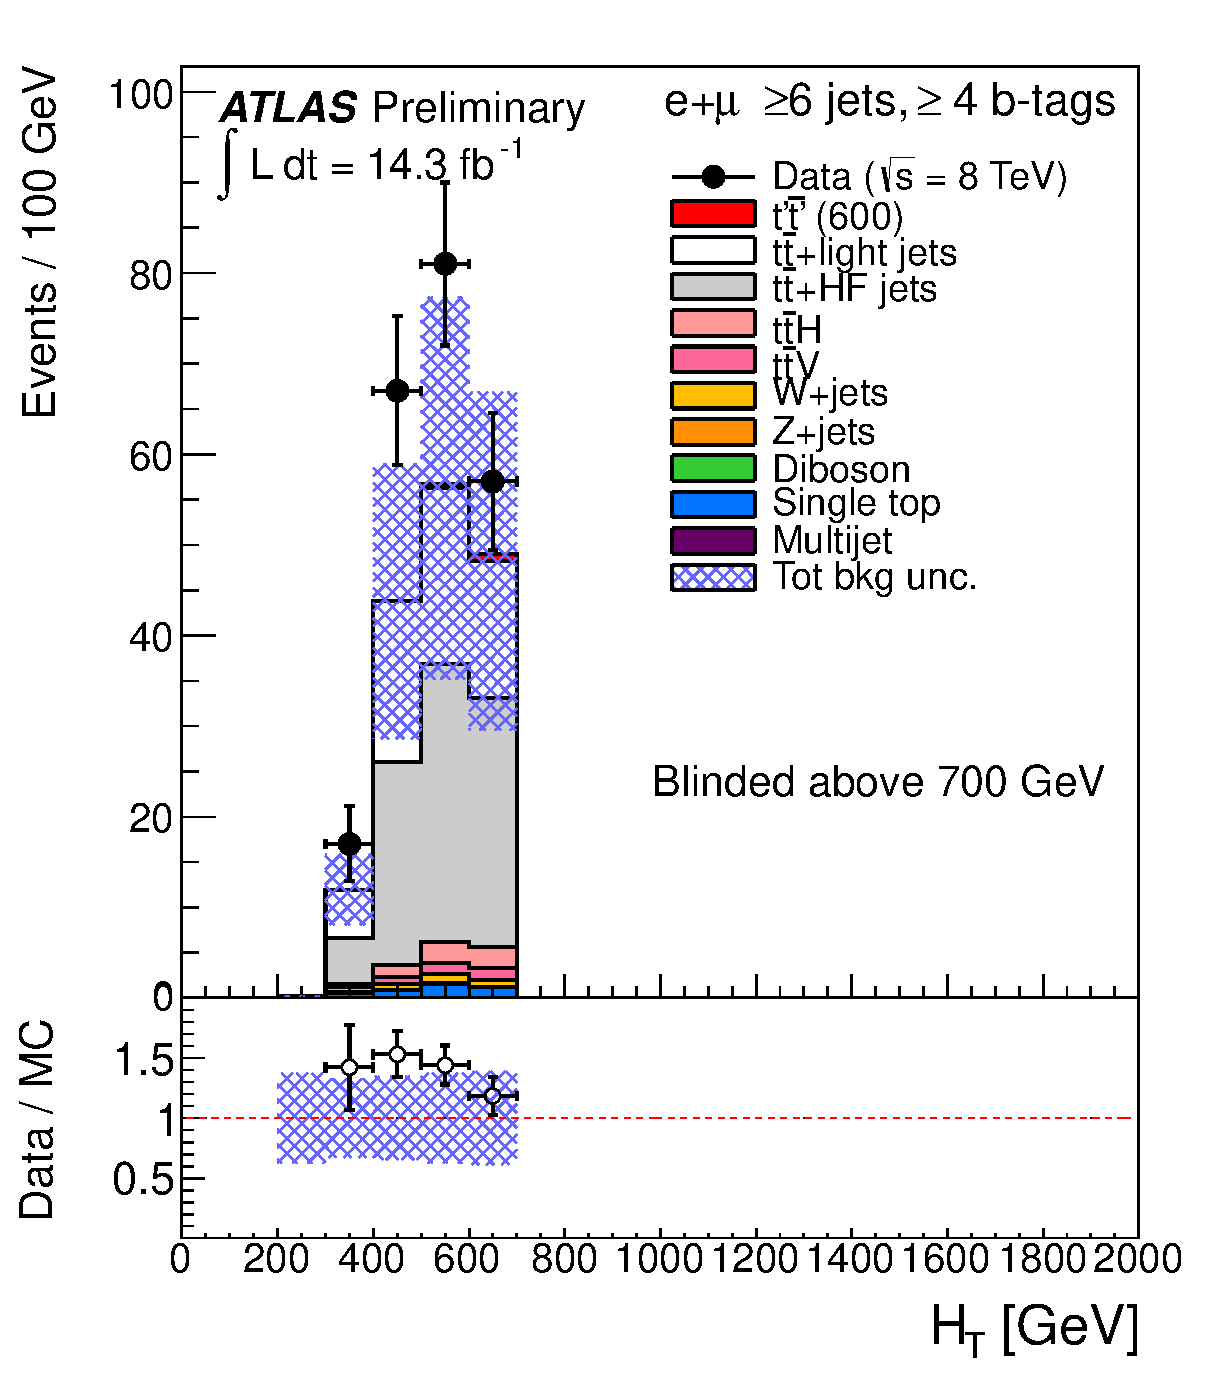
\includegraphics[width=0.3\textwidth]{htx_analysis_14ifb/figures/unscaled/HTAll_ELEMUON_6jetin4btagin_NOMINAL.eps}}
	\caption{Comparison of $\HT$ between data and simulation in the combined
electron and muon (a) \chii, (b) \chiii\ and (c) \chiv\ channels with 
the requirement of $\HT<700\gev$ to suppress a possible signal contribution.
The $t\bar{t}$+jets background is the nominal \texttt{ALPGEN} prediction before the fit to data (see text for details).
Also shown is the expected $\TT$ signal corresponding to $m_{\T}=600\gev$ in the $\T$ doublet scenario.
The bottom panel displays the ratio between data
and the background prediction. The shaded area represents the total background uncertainty.\label{fig:HT_beforefit}}
\end{center}\end{figure}
\begin{figure}[h!tb]\begin{center}
	\subfigure[]{\label{fig:scaled2}
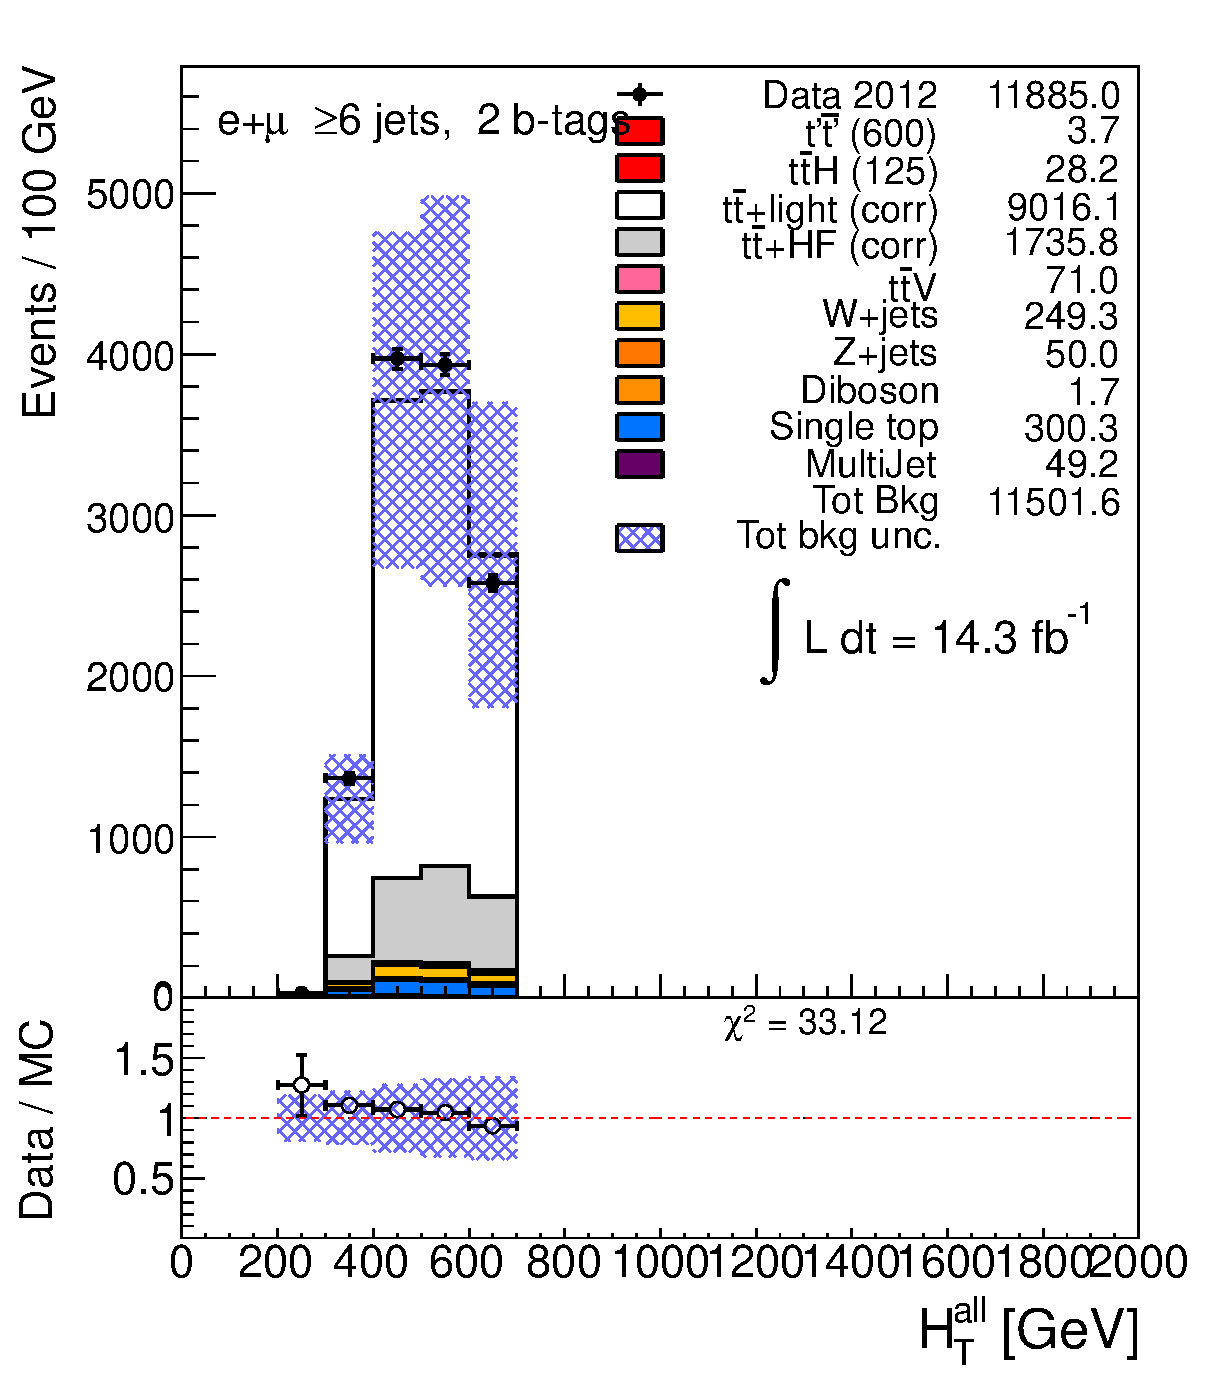
\includegraphics[width=0.3\textwidth]{htx_analysis_14ifb/figures/scaled/HTAll_ELEMUON_6jetin2btagex_NOMINAL.eps}}
	\subfigure[]{\label{fig:scaled3}
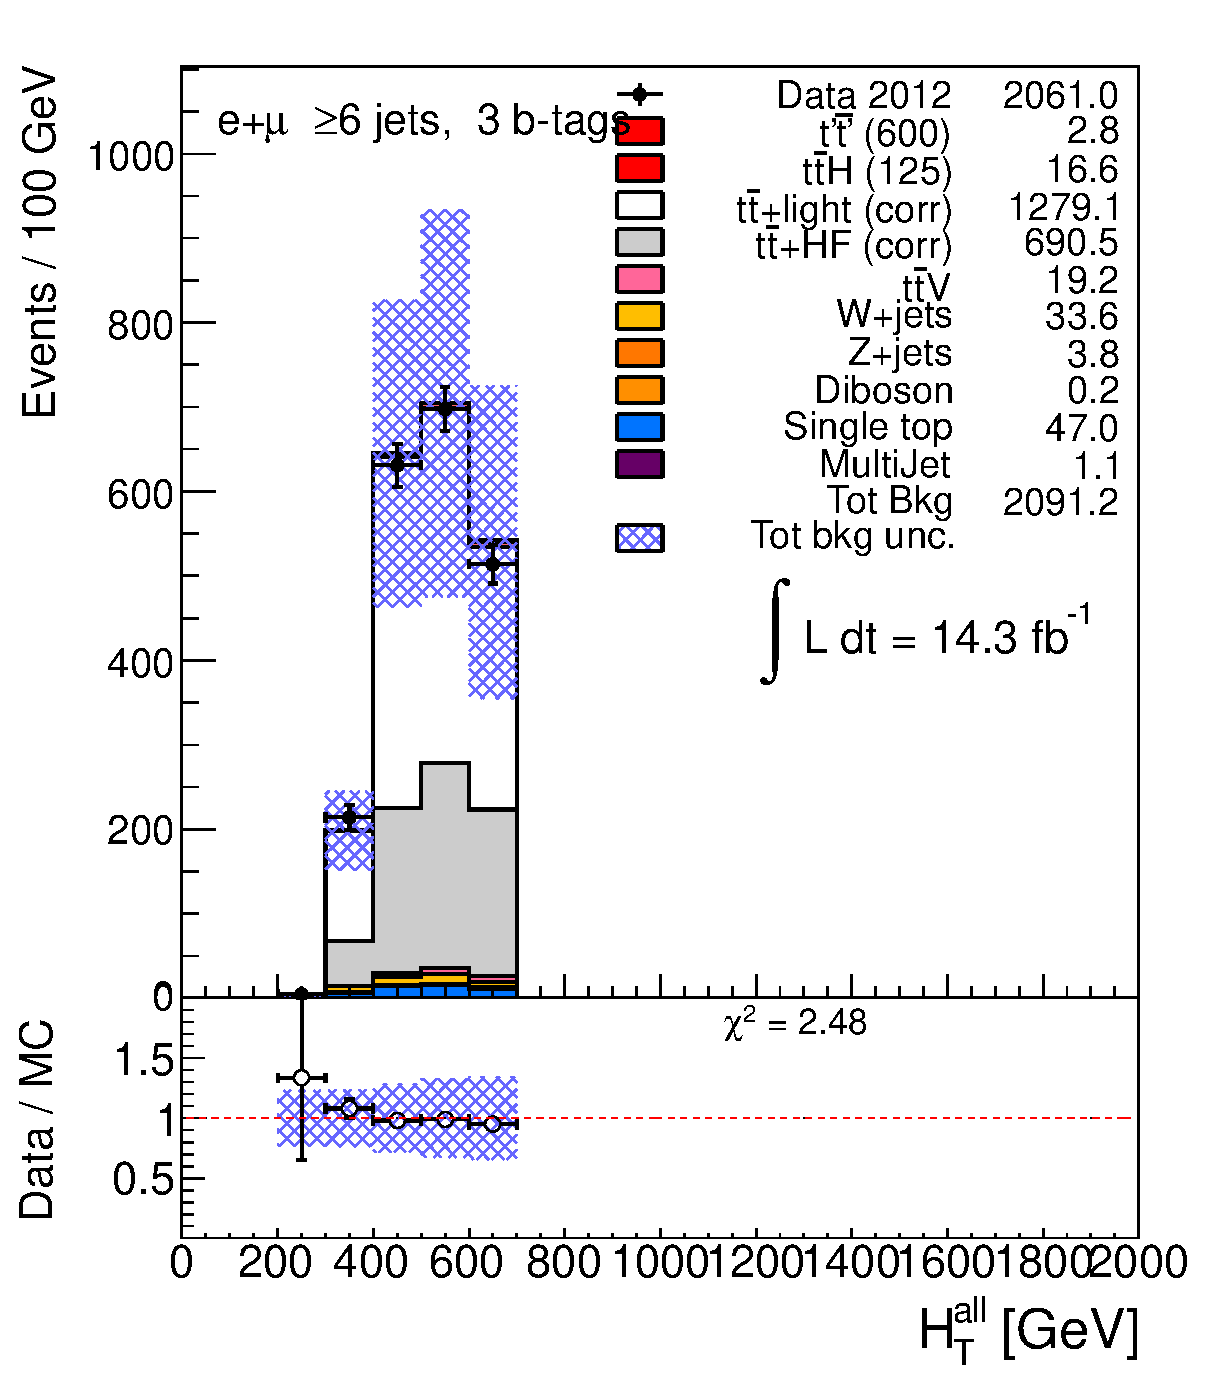
\includegraphics[width=0.3\textwidth]{htx_analysis_14ifb/figures/scaled/HTAll_ELEMUON_6jetin3btagex_NOMINAL.eps}}
	\subfigure[]{\label{fig:scaled4}
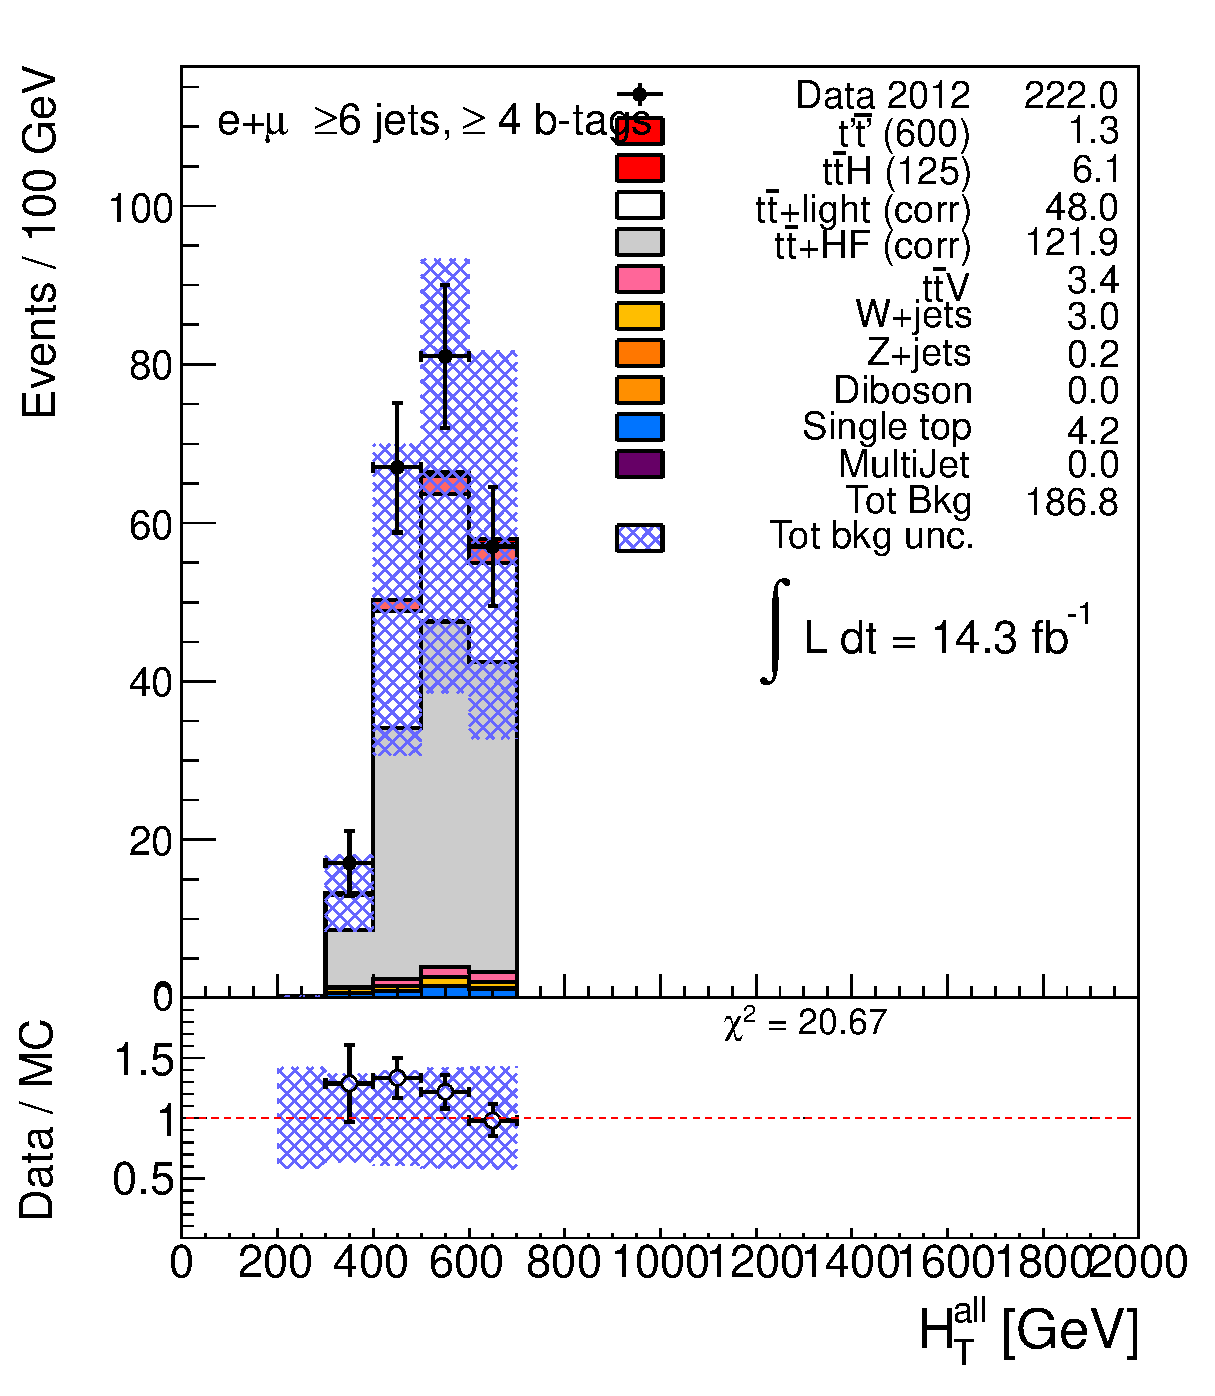
\includegraphics[width=0.3\textwidth]{htx_analysis_14ifb/figures/scaled/HTAll_ELEMUON_6jetin4btagin_NOMINAL.eps}}
	\caption{Comparison of $\HT$ between data and simulation in the combined
electron and muon (a) \chii, (b) \chiii\ and (c) \chiv\ channels with 
the requirement of $\HT<700\gev$ to suppress a possible signal contribution.
The $t\bar{t}$+jets background is the nominal \texttt{ALPGEN} prediction after the fit to data (see text for details).
Also shown is the expected $\TT$ signal corresponding to $m_{\T}=600\gev$ in the $\T$ doublet scenario.
The bottom panel displays the ratio between data
and the background prediction. The shaded area represents the total background uncertainty.\label{fig:HT_afterfit}}
\end{center}\end{figure}

In order to correct for the mismodeling of the $t\bar{t}$+jets 
Monte Carlo prediction from \texttt{ALPGEN} affecting in
particular the heavy-flavor component, two scaling factors are
introduced, one for \ttlf\ and one for \tthf, and are determined
by performing a simultaneous fit to the data distributions
of the $\HT$  variable in the three analysis channels. 
The measured scaling factors in the blinded channels are 
$0.87 \pm 0.02\,{\rm (stat.)}$ for \ttlf\ and 
$1.35 \pm 0.11\,{\rm (stat.)}$ for \tthf.
The $\HT$ distributions in the \chii, \chiii\ and \chiv\ 
channels corresponding to the total background contributions
before and after the scaling are compared in Figure
\begin{figure}[htb]\begin{center}
	\subfigure[]{
  	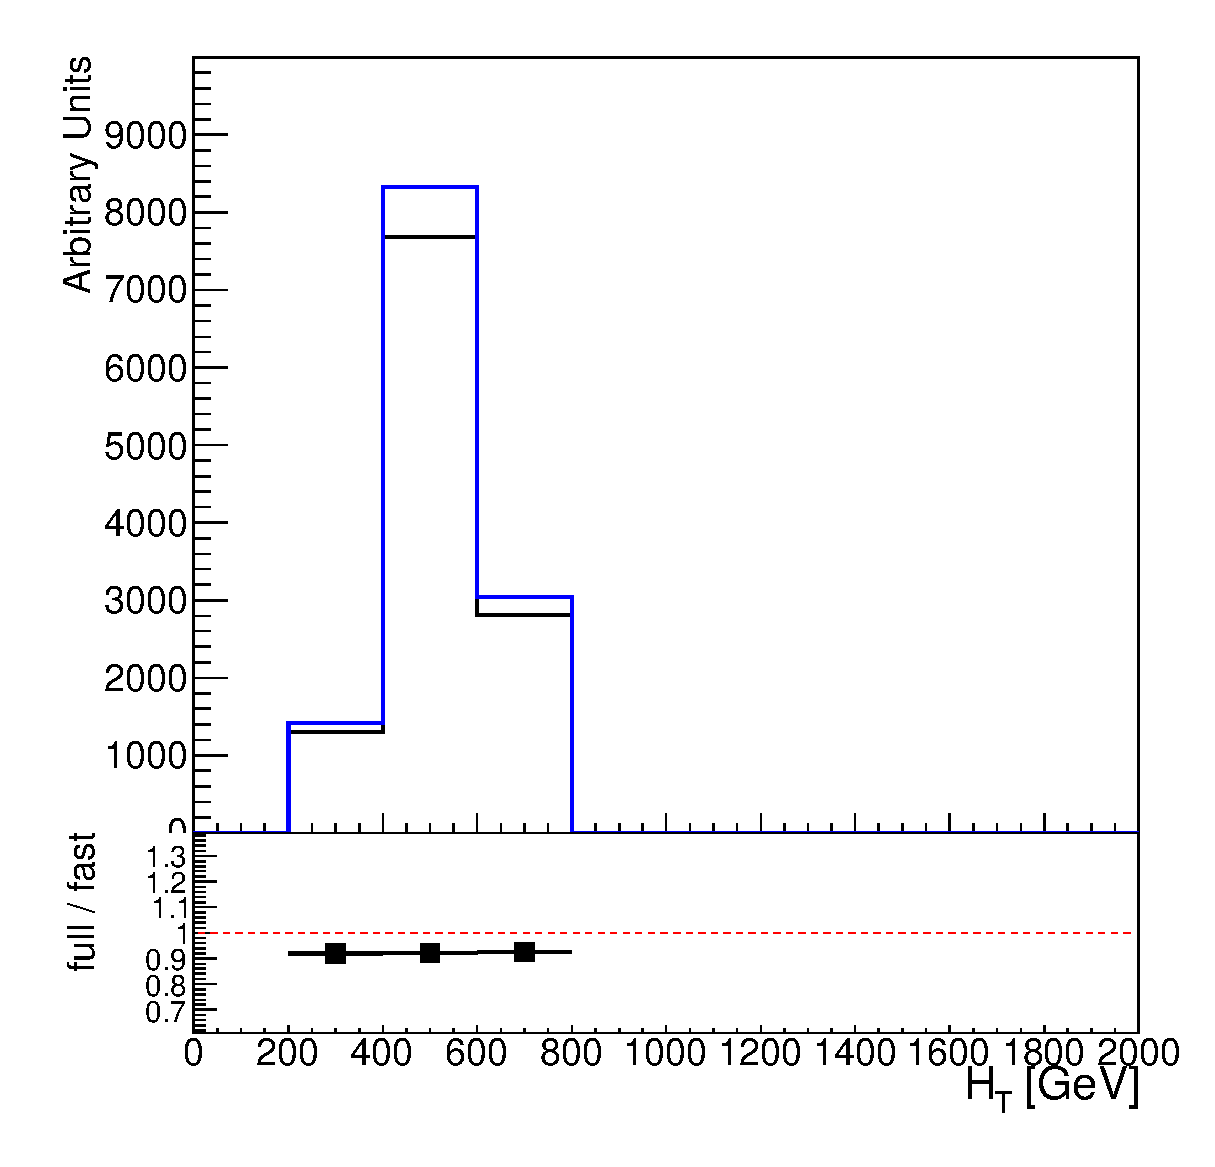
\includegraphics[width=0.3\textwidth]{htx_analysis_14ifb/figures/scaling_HTAll_ELEMUON_6jetin2btagex_NOMINAL}}
	\subfigure[]{
  	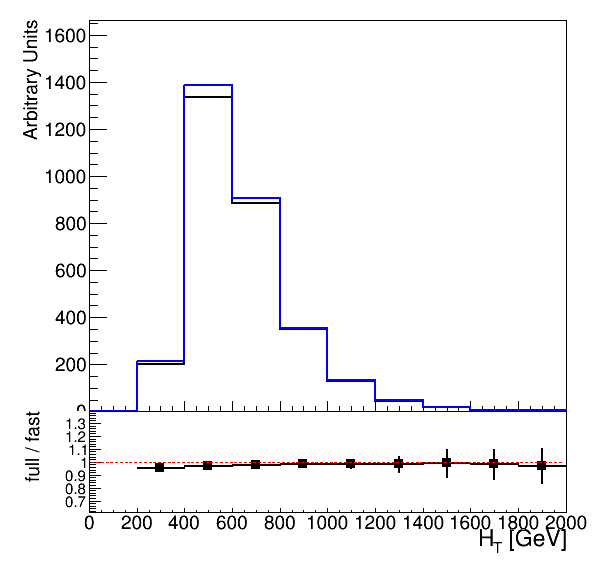
\includegraphics[width=0.3\textwidth]{htx_analysis_14ifb/figures/scaling_HTAll_ELEMUON_6jetin3btagex_NOMINAL}}
	\subfigure[]{
  	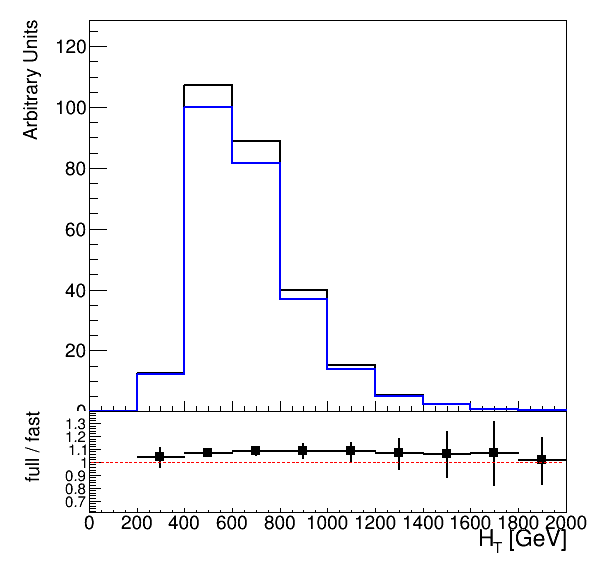
\includegraphics[width=0.3\textwidth]{htx_analysis_14ifb/figures/scaling_HTAll_ELEMUON_6jetin4btagin_NOMINAL}}
	\caption{Comparison of the  $\HT$  variable shape and normalization for the
        total backgrounds in the (a) \chii, (b) \chiii, (c) \chiv\ channels, with and
        without applying the rescaling to the \ttlf\ and \tthf\ contributions. \label{fig:htcomp}}
\end{center}\end{figure}
The distributions obtained after applying this scaling
to the \texttt{ALPGEN} prediction are shown in Figure~\ref{fig:HT_afterfit}.
This rescaled prediction is taken as default from now on, and
Figure~\ref{fig:htxCRs} shows the agreement between data and
backgrond prediction in the three blinded analysis channels.


\begin{figure}[h!tb]\begin{center}
	\subfigure[]{
  	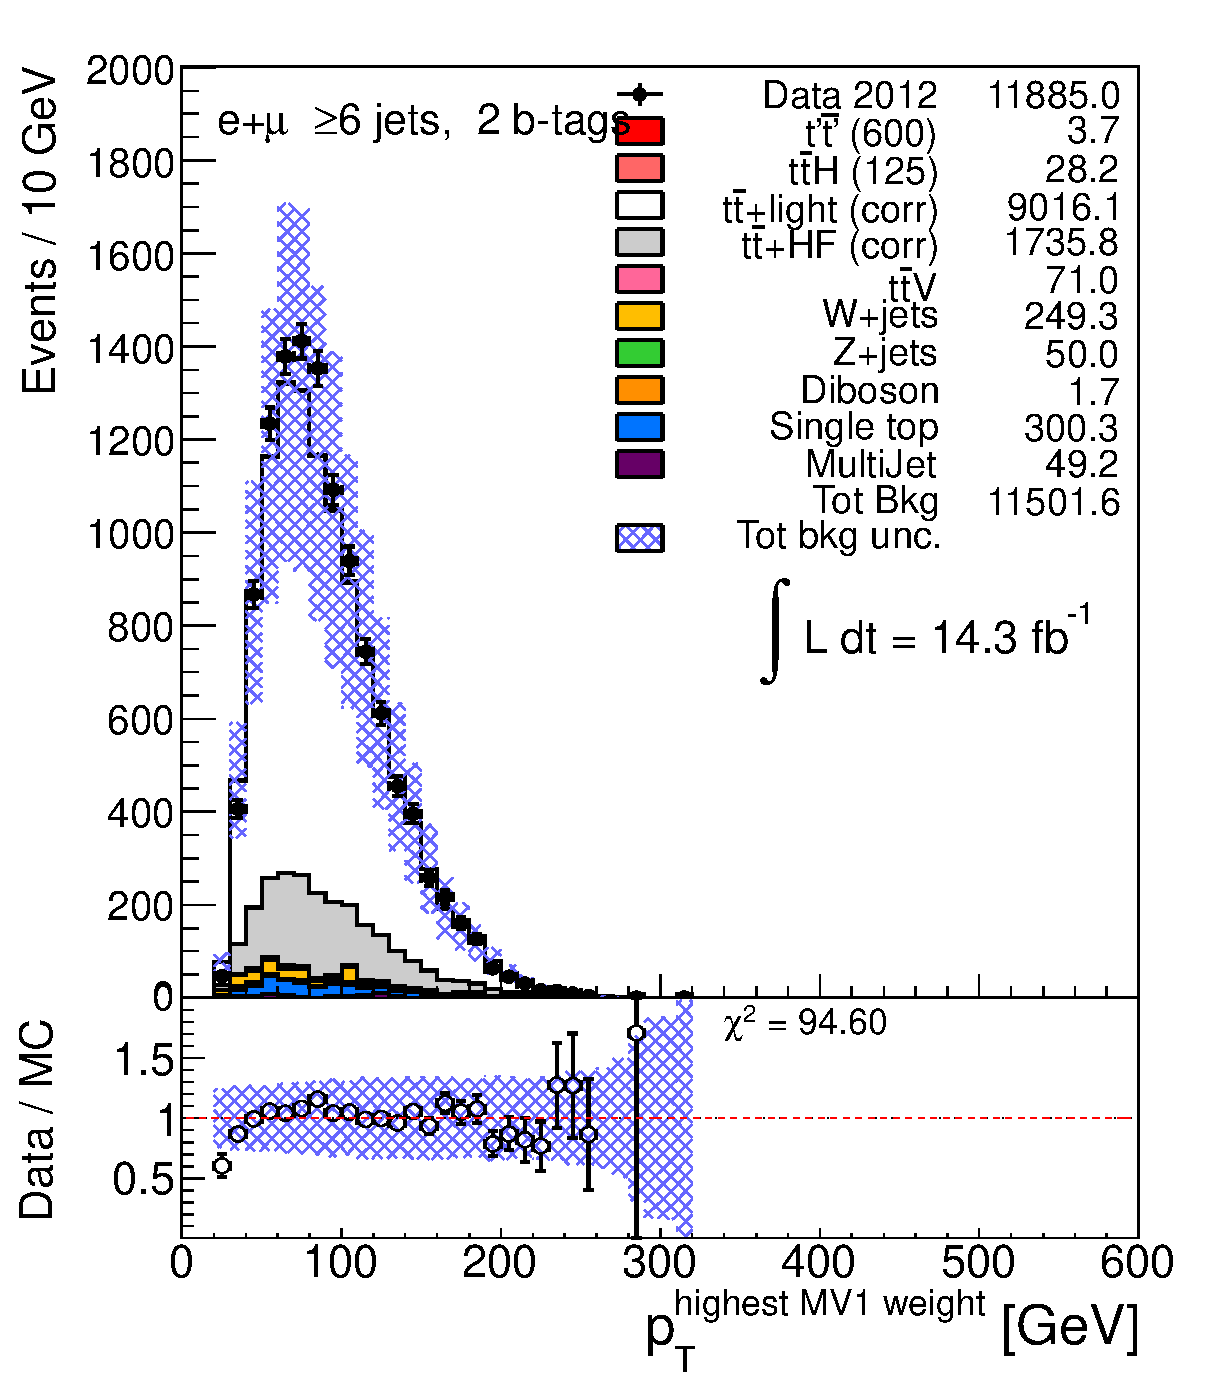
\includegraphics[width=0.235\textwidth]{htx_analysis_14ifb/figures/scaled_cr_blind/JetPtB1_ELEMUON_6jetin2btagex_NOMINAL}}
	\subfigure[]{
  	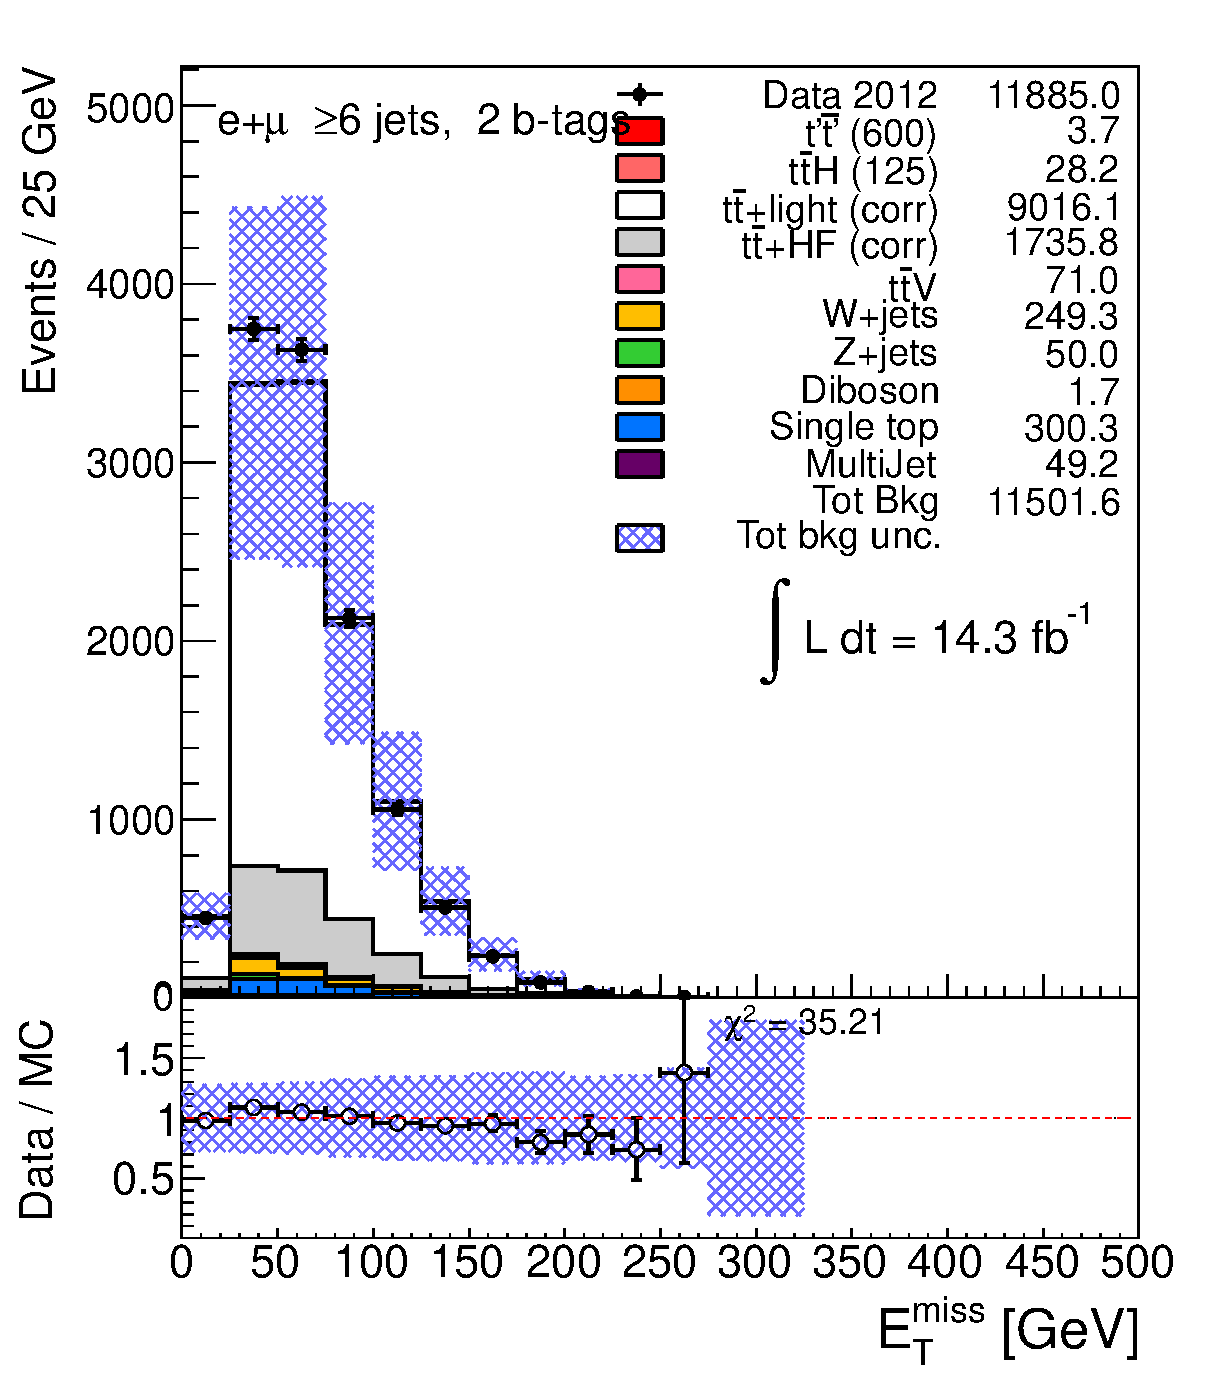
\includegraphics[width=0.235\textwidth]{htx_analysis_14ifb/figures/scaled_cr_blind/MET_ELEMUON_6jetin2btagex_NOMINAL}}
	\subfigure[]{
  	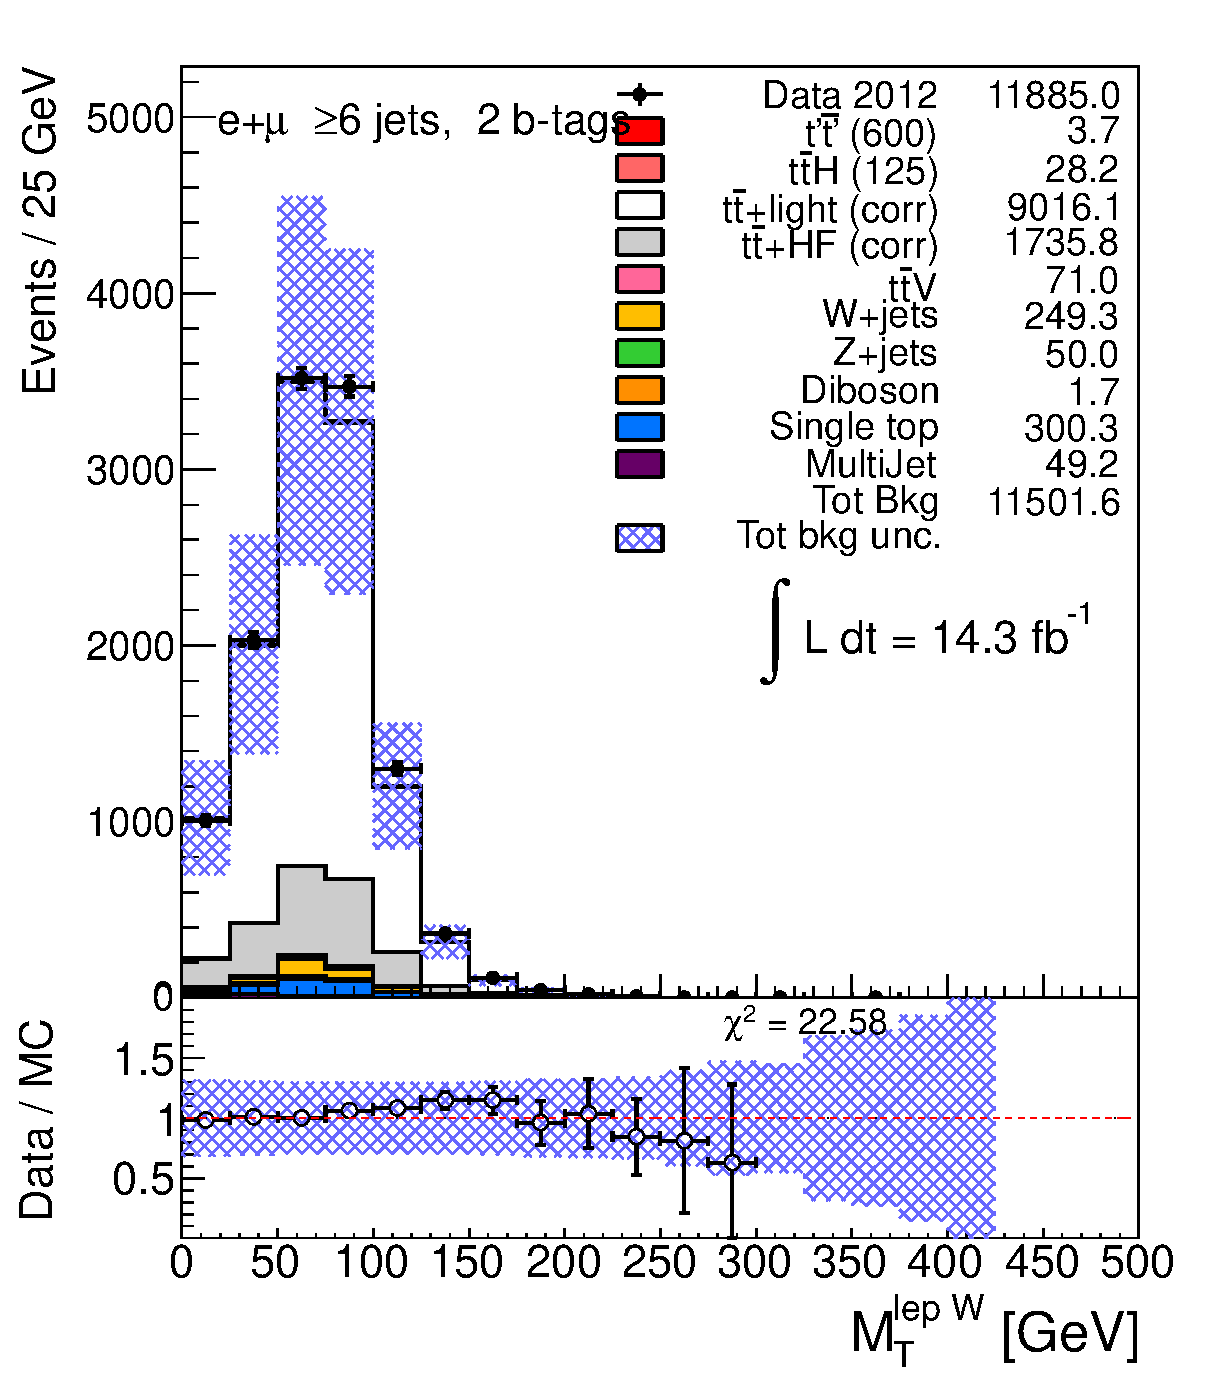
\includegraphics[width=0.235\textwidth]{htx_analysis_14ifb/figures/scaled_cr_blind/Wlep_MassT_ELEMUON_6jetin2btagex_NOMINAL}}
	\subfigure[]{
  	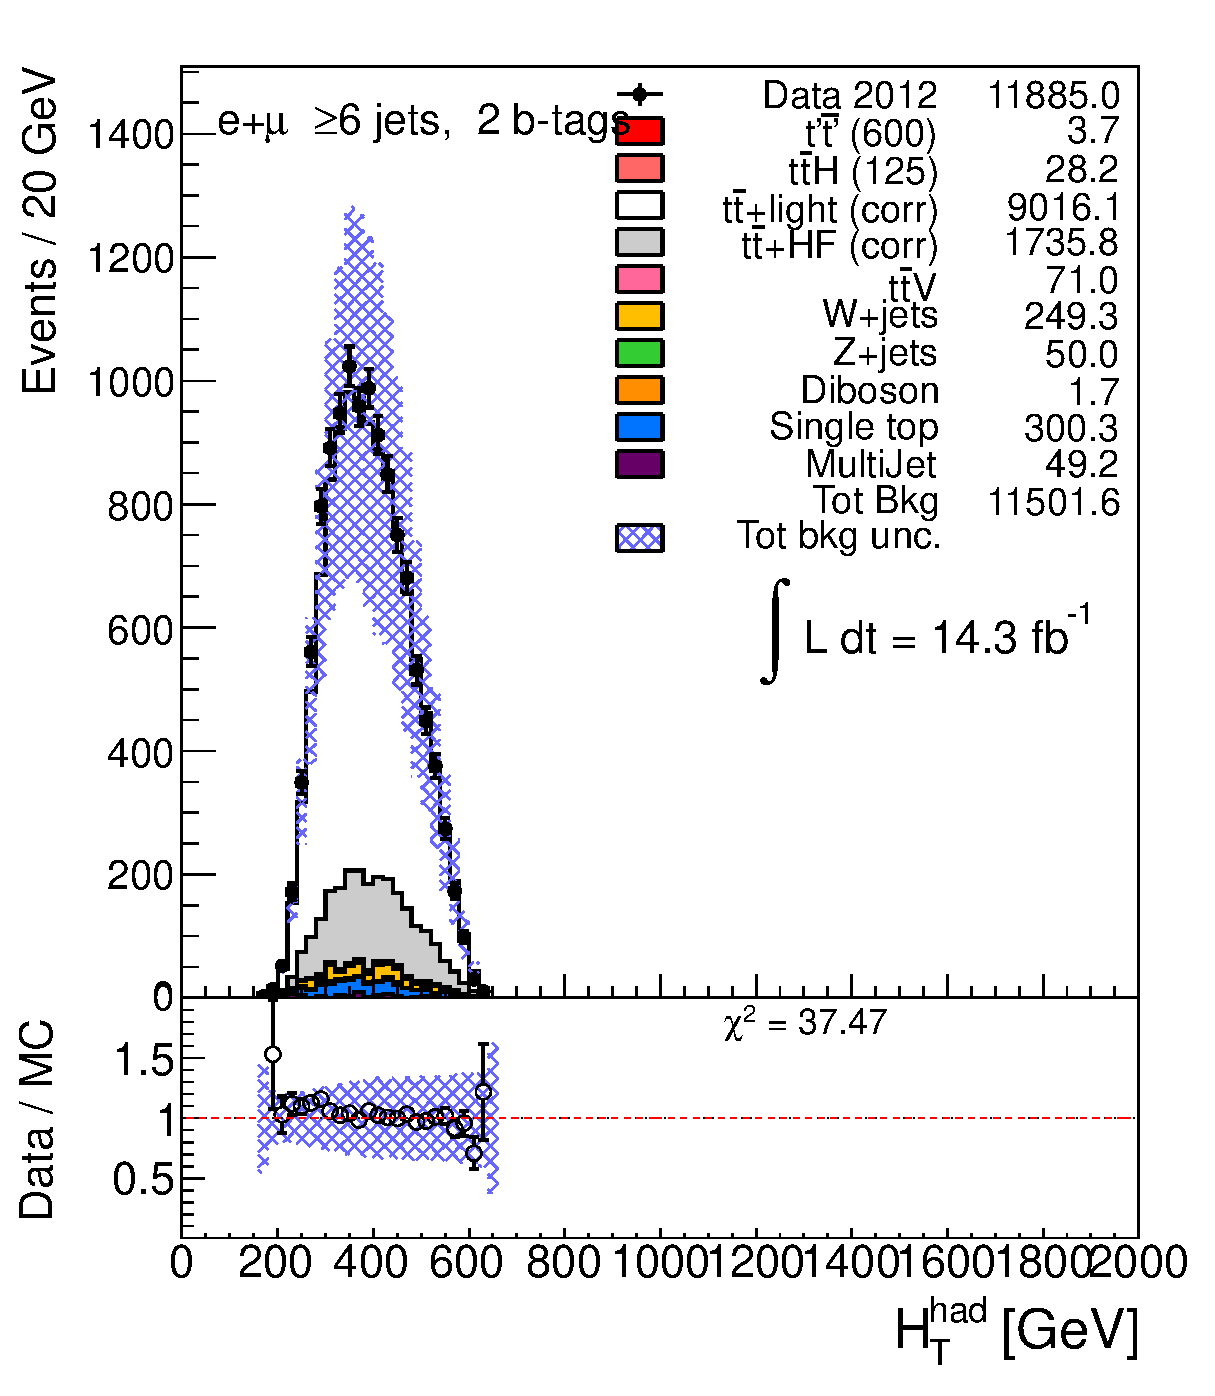
\includegraphics[width=0.235\textwidth]{htx_analysis_14ifb/figures/scaled_cr_blind/HTHad_ELEMUON_6jetin2btagex_NOMINAL}}\\
	\subfigure[]{
  	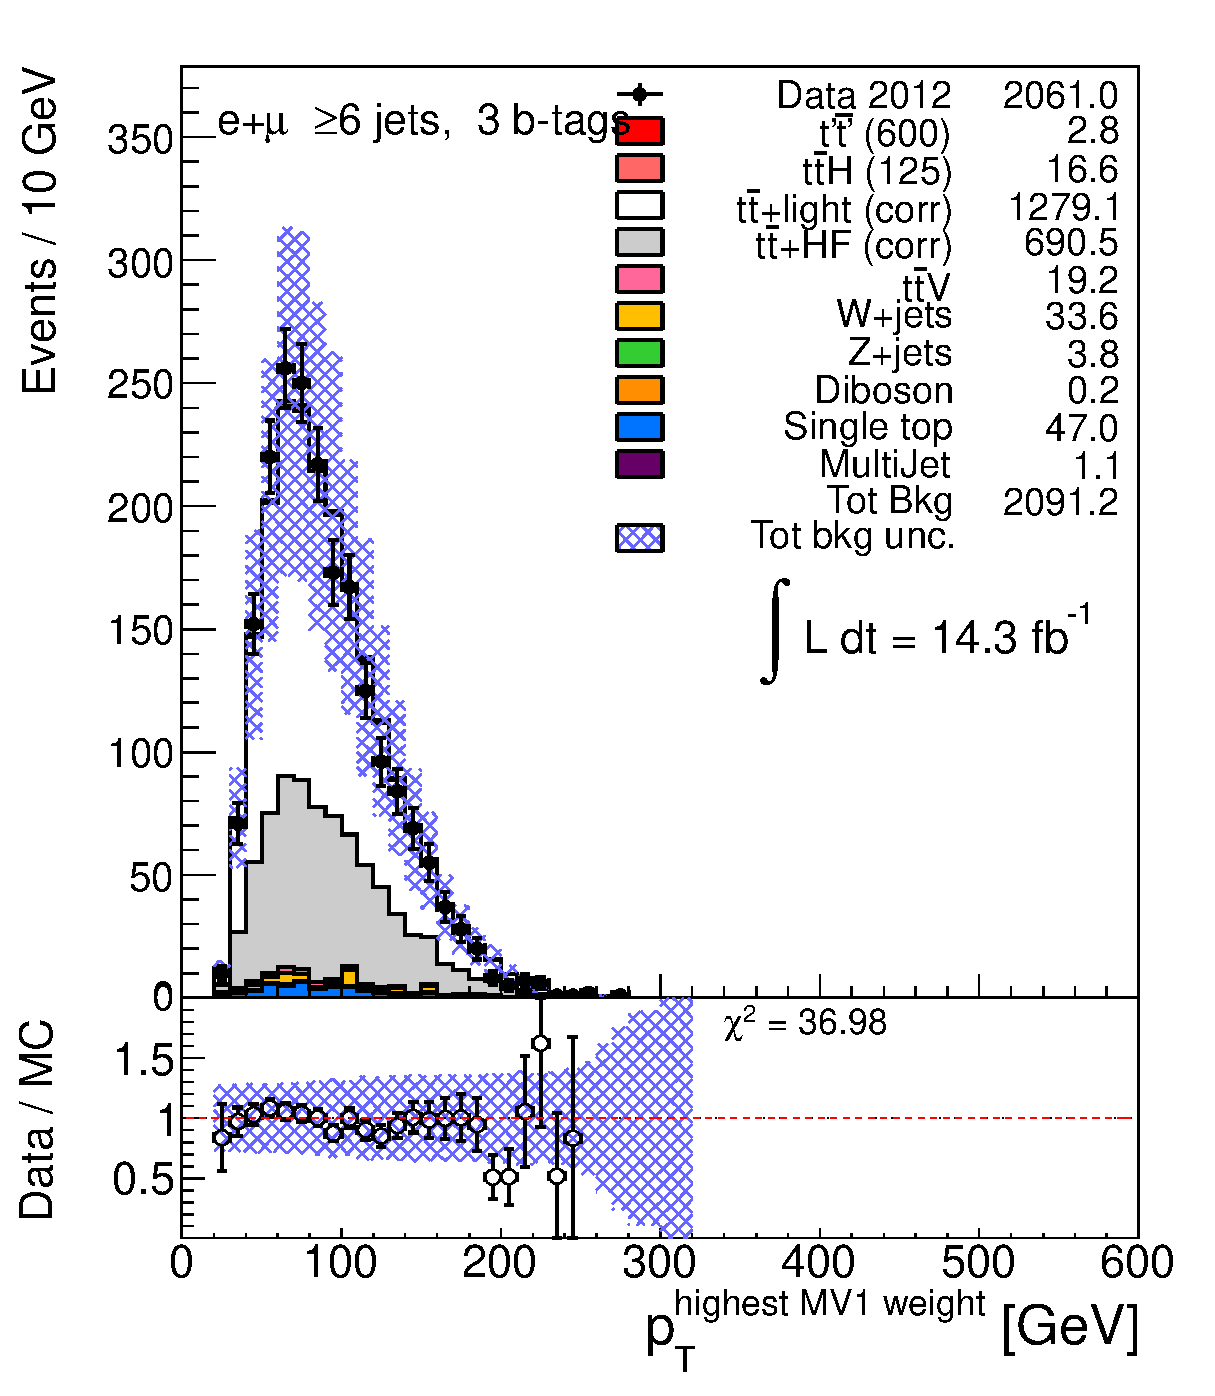
\includegraphics[width=0.235\textwidth]{htx_analysis_14ifb/figures/scaled_cr_blind/JetPtB1_ELEMUON_6jetin3btagex_NOMINAL}}
	\subfigure[]{
  	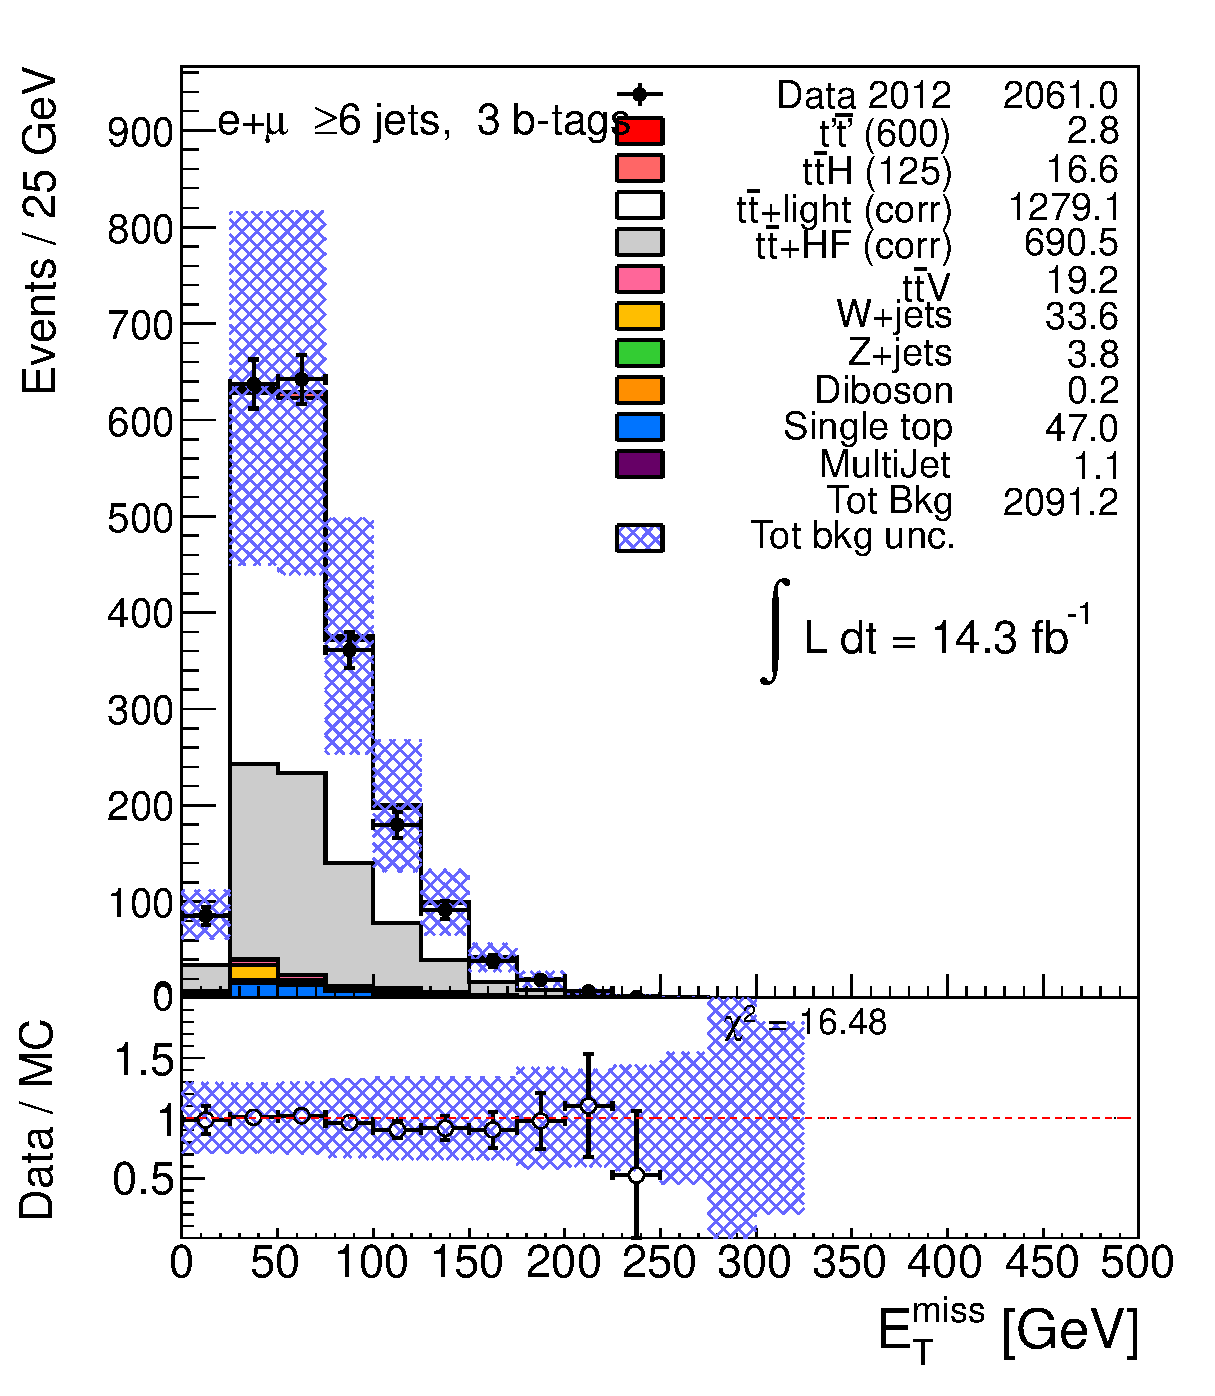
\includegraphics[width=0.235\textwidth]{htx_analysis_14ifb/figures/scaled_cr_blind/MET_ELEMUON_6jetin3btagex_NOMINAL}}
	\subfigure[]{
  	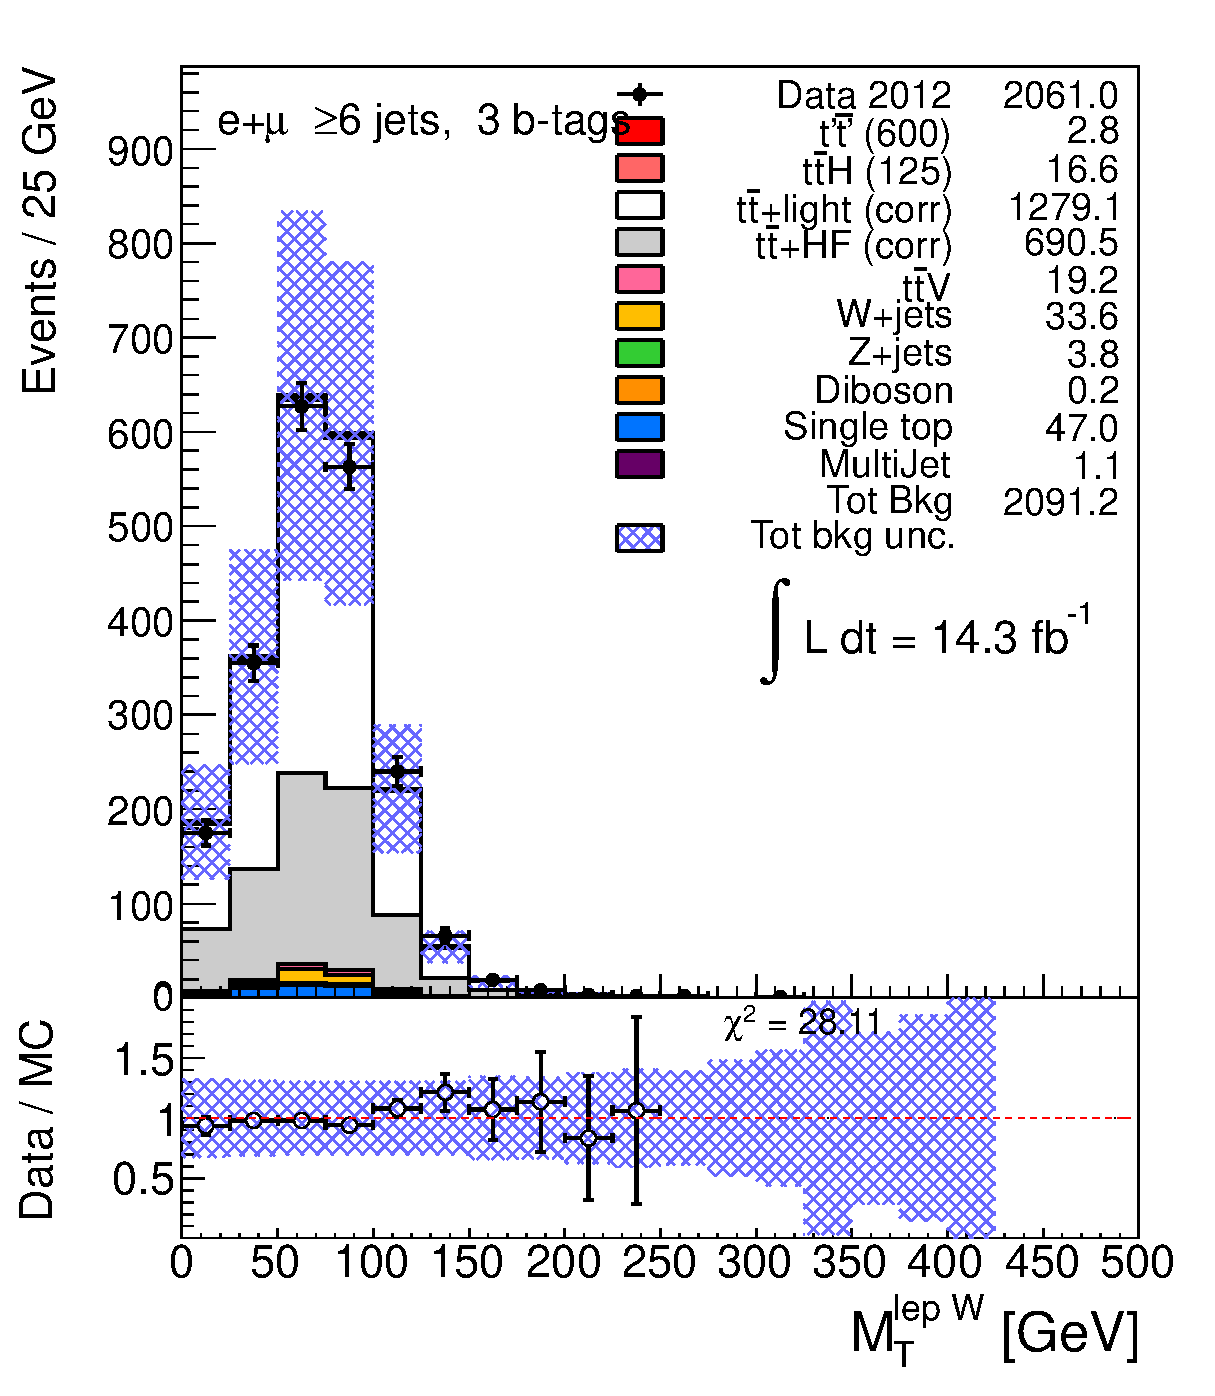
\includegraphics[width=0.235\textwidth]{htx_analysis_14ifb/figures/scaled_cr_blind/Wlep_MassT_ELEMUON_6jetin3btagex_NOMINAL}}
	\subfigure[]{
  	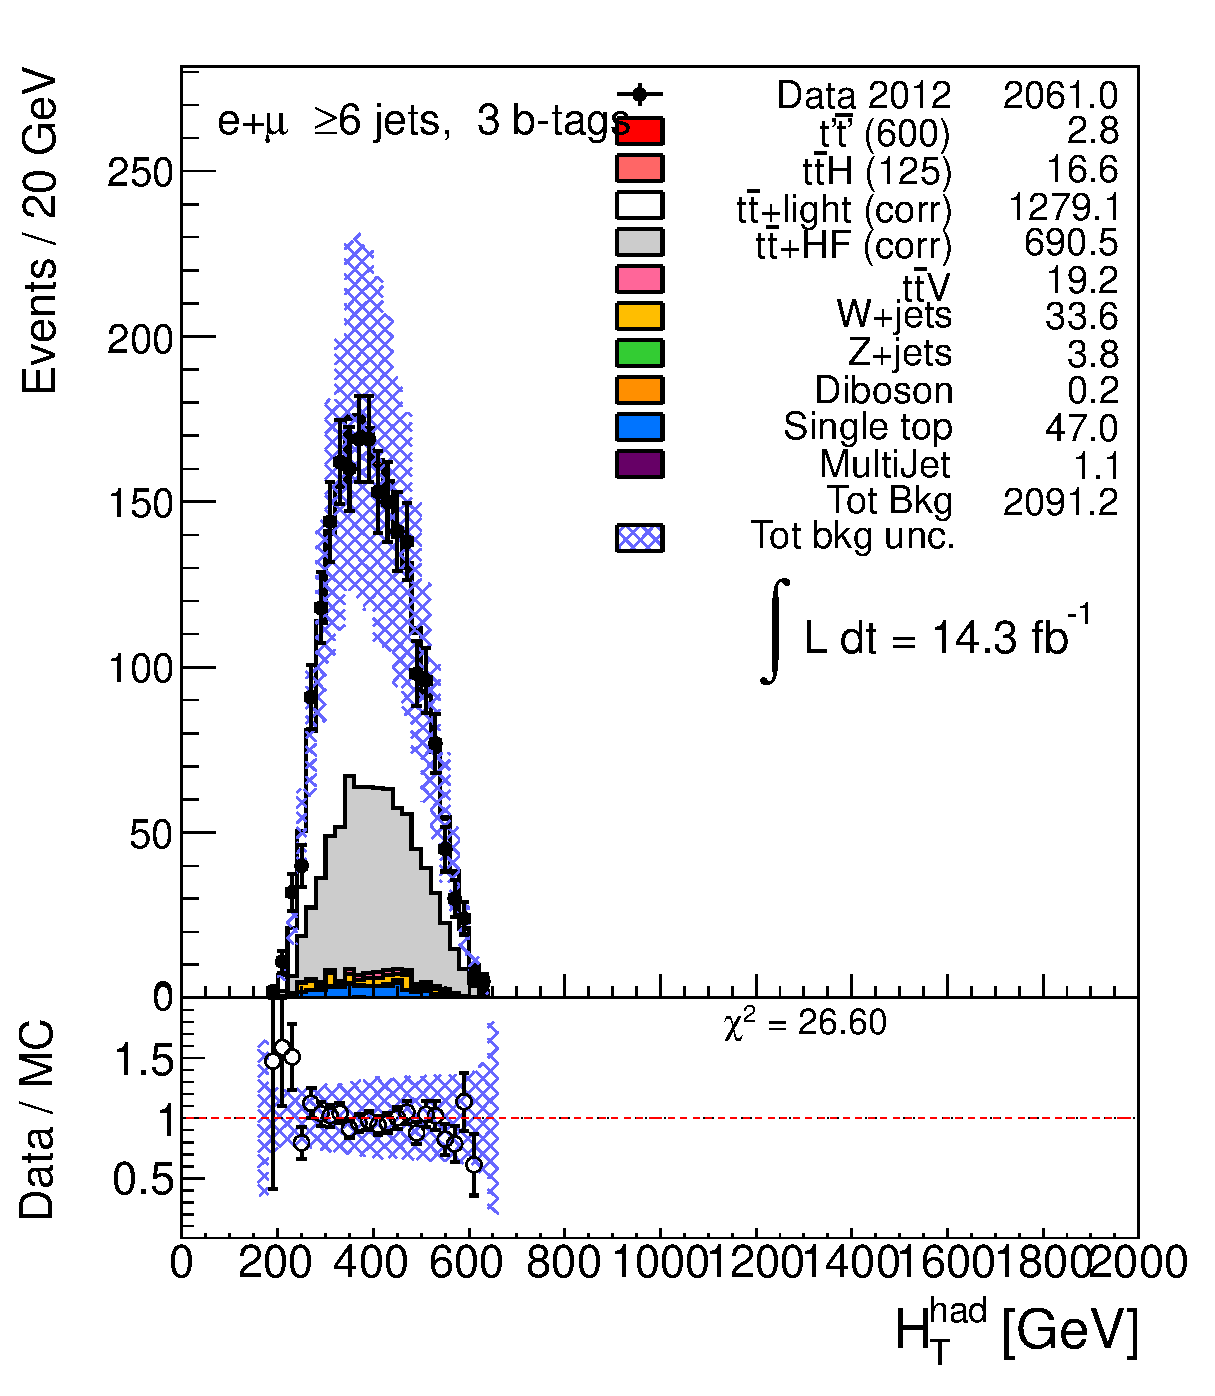
\includegraphics[width=0.235\textwidth]{htx_analysis_14ifb/figures/scaled_cr_blind/HTHad_ELEMUON_6jetin3btagex_NOMINAL}}\\
	\subfigure[]{
  	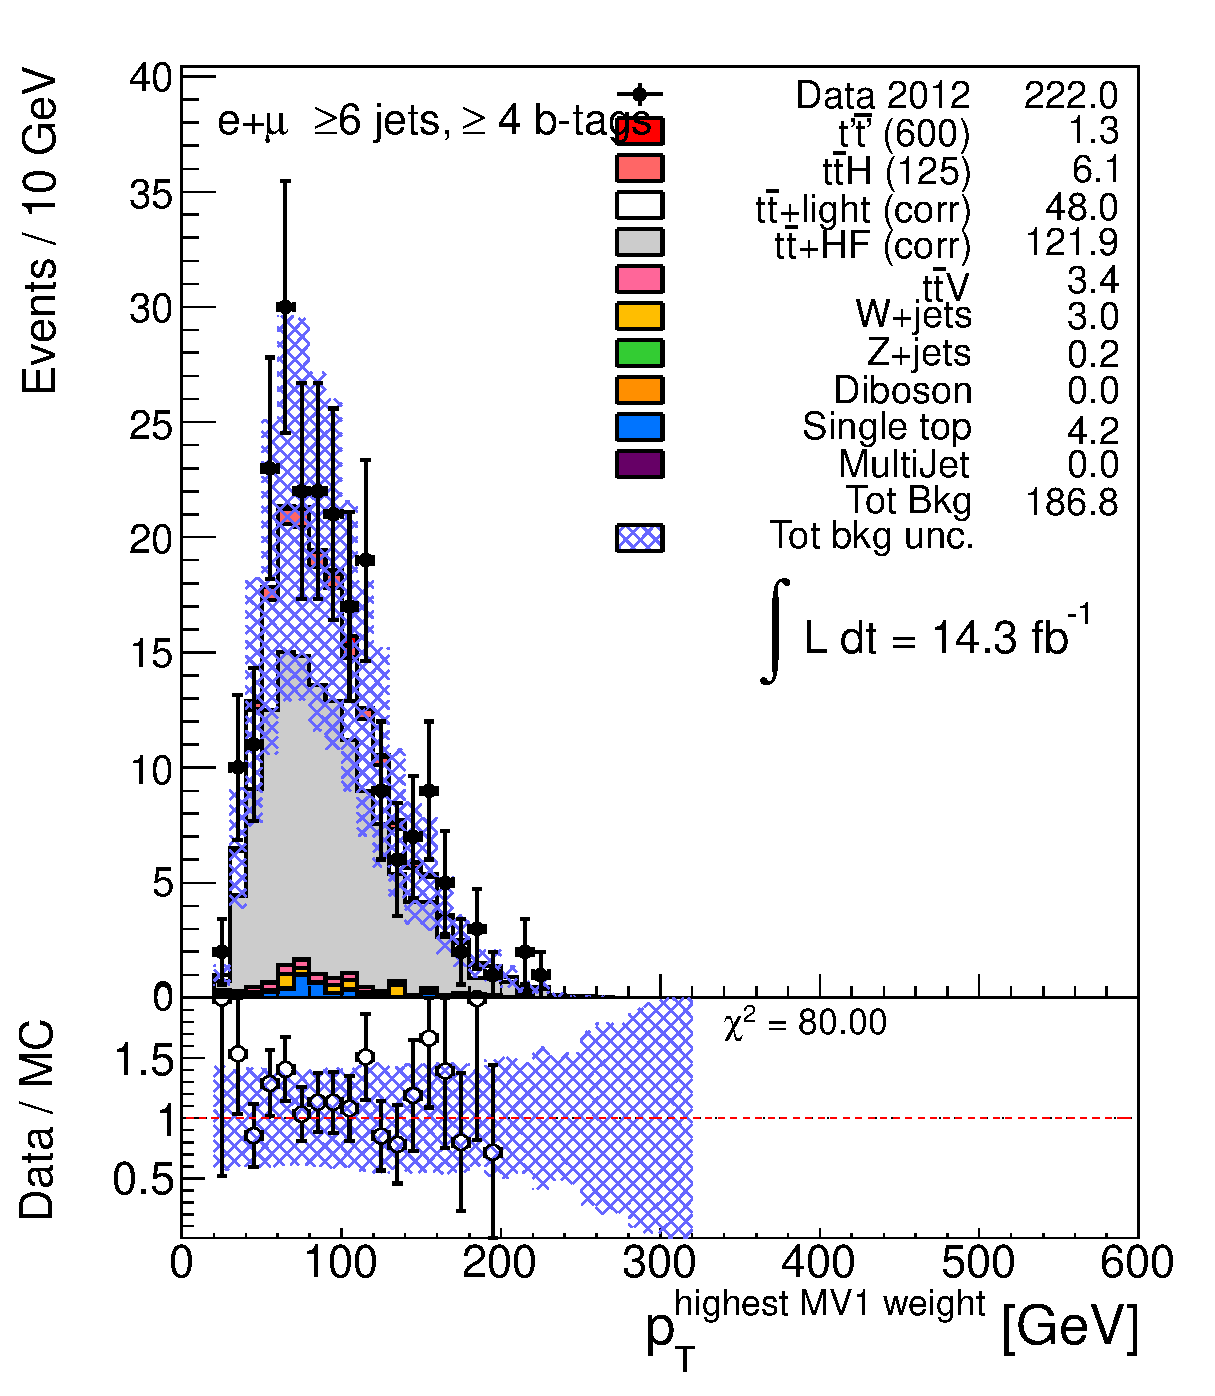
\includegraphics[width=0.235\textwidth]{htx_analysis_14ifb/figures/scaled_cr_blind/JetPtB1_ELEMUON_6jetin4btagin_NOMINAL}}
	\subfigure[]{
  	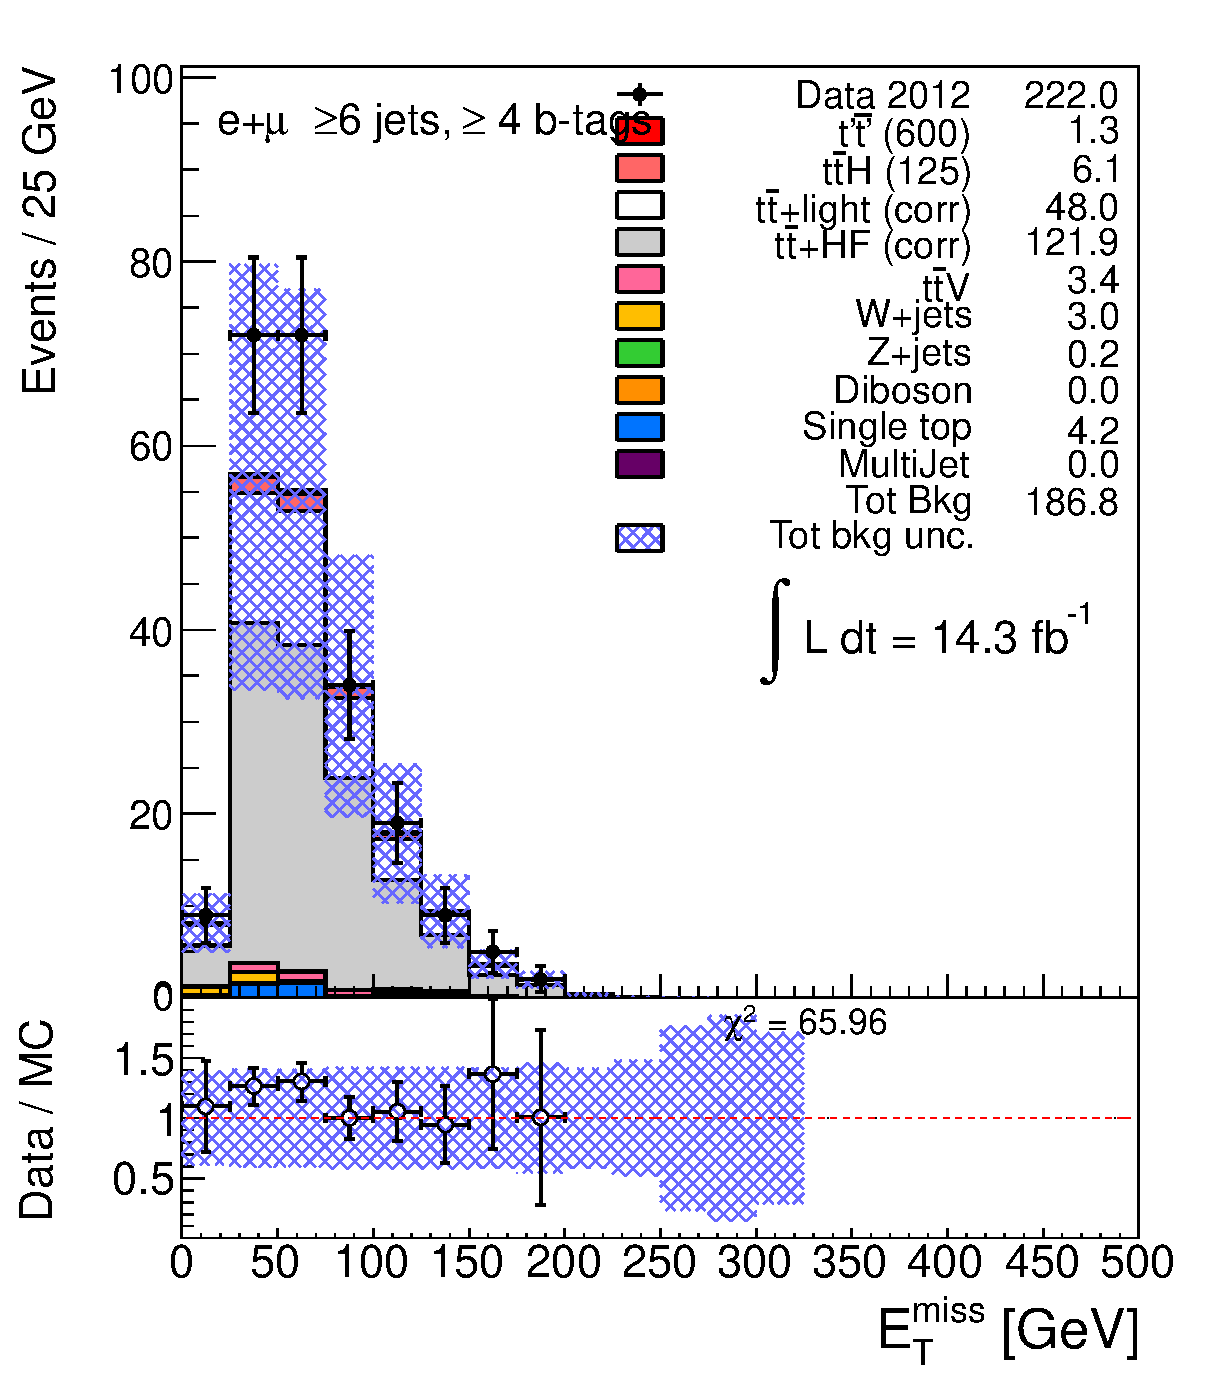
\includegraphics[width=0.235\textwidth]{htx_analysis_14ifb/figures/scaled_cr_blind/MET_ELEMUON_6jetin4btagin_NOMINAL}}
	\subfigure[]{
  	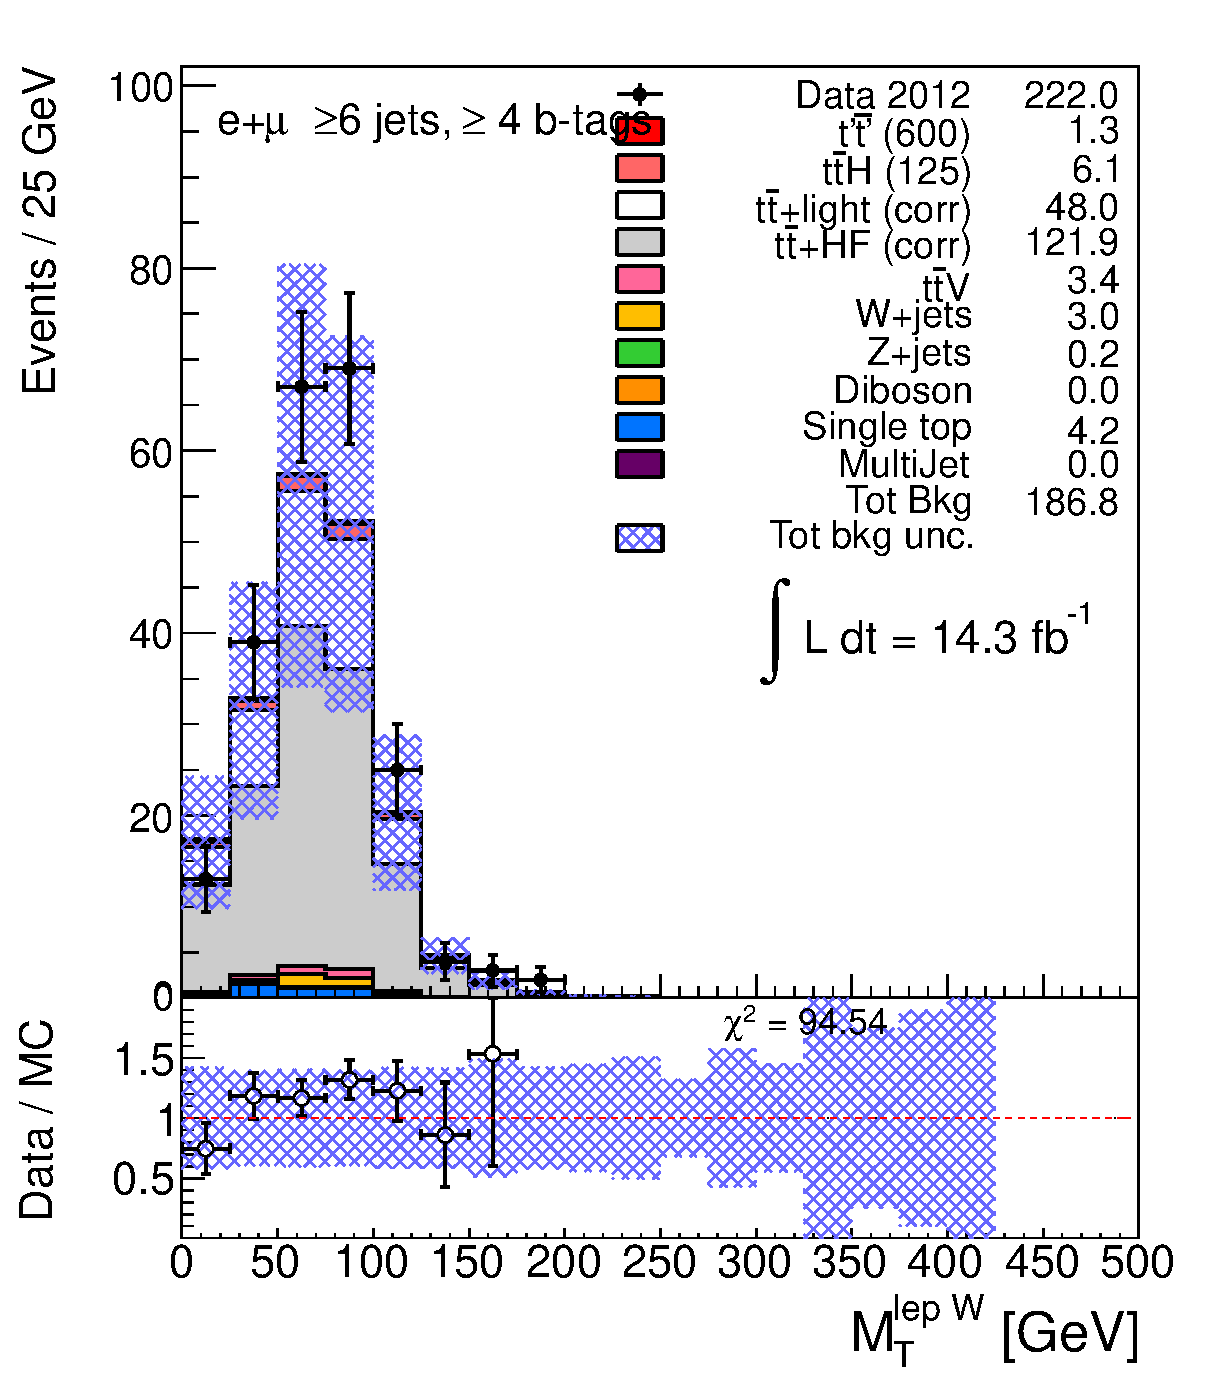
\includegraphics[width=0.235\textwidth]{htx_analysis_14ifb/figures/scaled_cr_blind/Wlep_MassT_ELEMUON_6jetin4btagin_NOMINAL}}
	\subfigure[]{
  	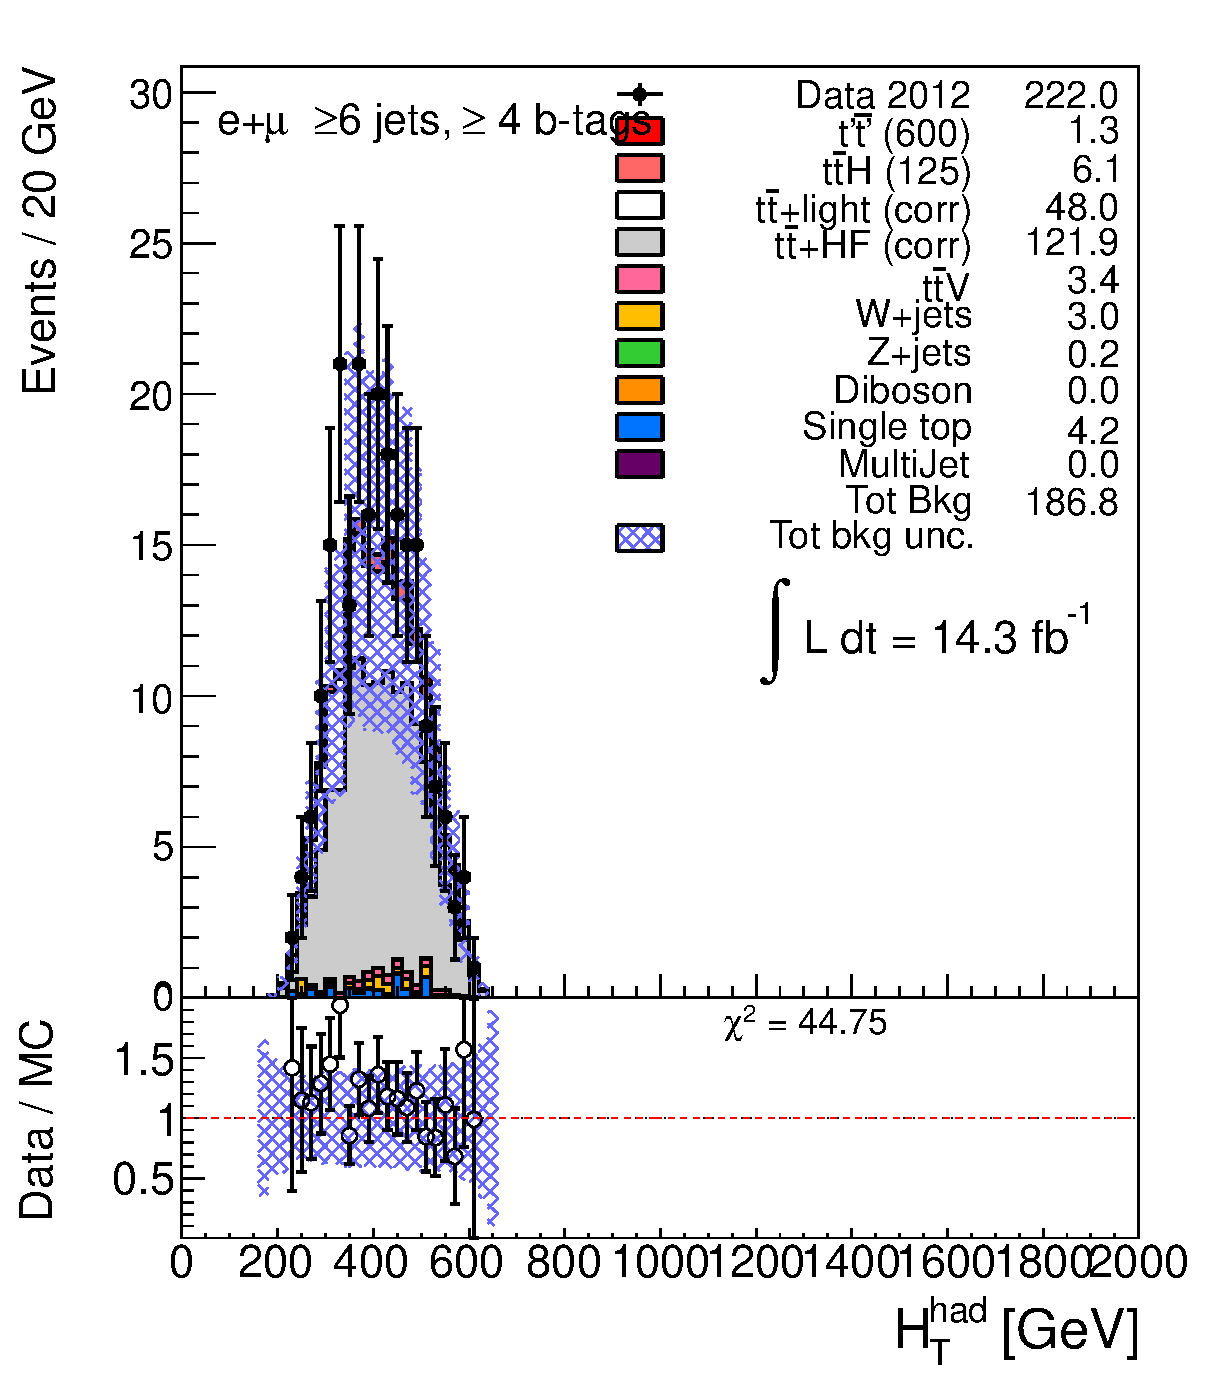
\includegraphics[width=0.235\textwidth]{htx_analysis_14ifb/figures/scaled_cr_blind/HTHad_ELEMUON_6jetin4btagin_NOMINAL}}\\
	\caption{Comparison of various distributions between data and simulation in the combined
$e$+jets and $\mu$+jets (a-d) \chii, (e-h) \chiii\ and (i-l) \chiv\ channels with 
the requirement of $\HT<700\gev$ to suppress a possible signal contribution.
The variables are, from left to right: \pt\ of the jet with the highest MV1 weight;
missing tranverse energy; transverse mass of $W$ boson; hadronic component of \HT.
The $t\bar{t}$+jets background is the nominal \texttt{ALPGEN} prediction after the fit to data (see text for details).
Also shown is the expected $\TT$ signal corresponding to $m_{\T}=600\gev$ in the $\T$ doublet scenario.
The bottom panel displays the ratio between data
and the background prediction. The shaded area represents the total background uncertainty.\label{fig:htxCRs}}
\end{center}\end{figure}



Considering that the previously defined control regions do not allow
to investigate the data to Standard Model backgrounds comparison in
the tails of the $\HT$ distribution where the eventual signal would lay,
an additional control region is defined as follows: 
at most two jets with $\pt>60\gev$, $\HT<1.2\tev$, and either 2 or 3 \btag ged jets.
The  $\geq 4$ \btag ged jets is not considered as it still has 
a large signal content and too low background statistics to provide
a useful cross-check.
A comparison between data and simulation for the $\HT$ distribution 
in these two additional control regions is shown in 
Figure~\ref{fig:HT_signalregion_control}. More details are given 
in Appendix~\ref{app:htx_httail}.
%for the 2 $b$-tags and 3 $b$-tags channels.
%Further details can be found in App.~\ref{sec:httails_controlregions}.
Data are found to be in reasonable agreement with the 
prediction within the assigned systematic uncertainties. 
The last two bins of Figure~\ref{fig:httail3} have too low
statistics (10 and 1 data events) for their error to be properly computed.
%While some systematic discrepancy, still within the systematic uncertainty band, is obvious in the 2 $b$-tags channel, it is less apparent in the 3 $b$-tags channel. In the latter, the last two bins outside the uncertainty band have  10 and 1 data events, respectively, so statistical uncertainties are not properly computed. Also, the MC prediction  appears to have significant statistical fluctuations (see e.g. $W$+jets template). More details can be found in App.~\ref{sec:httails_controlregions}.

\begin{figure}[htb]\begin{center}
	\subfigure[]{\label{fig:httail2}
  	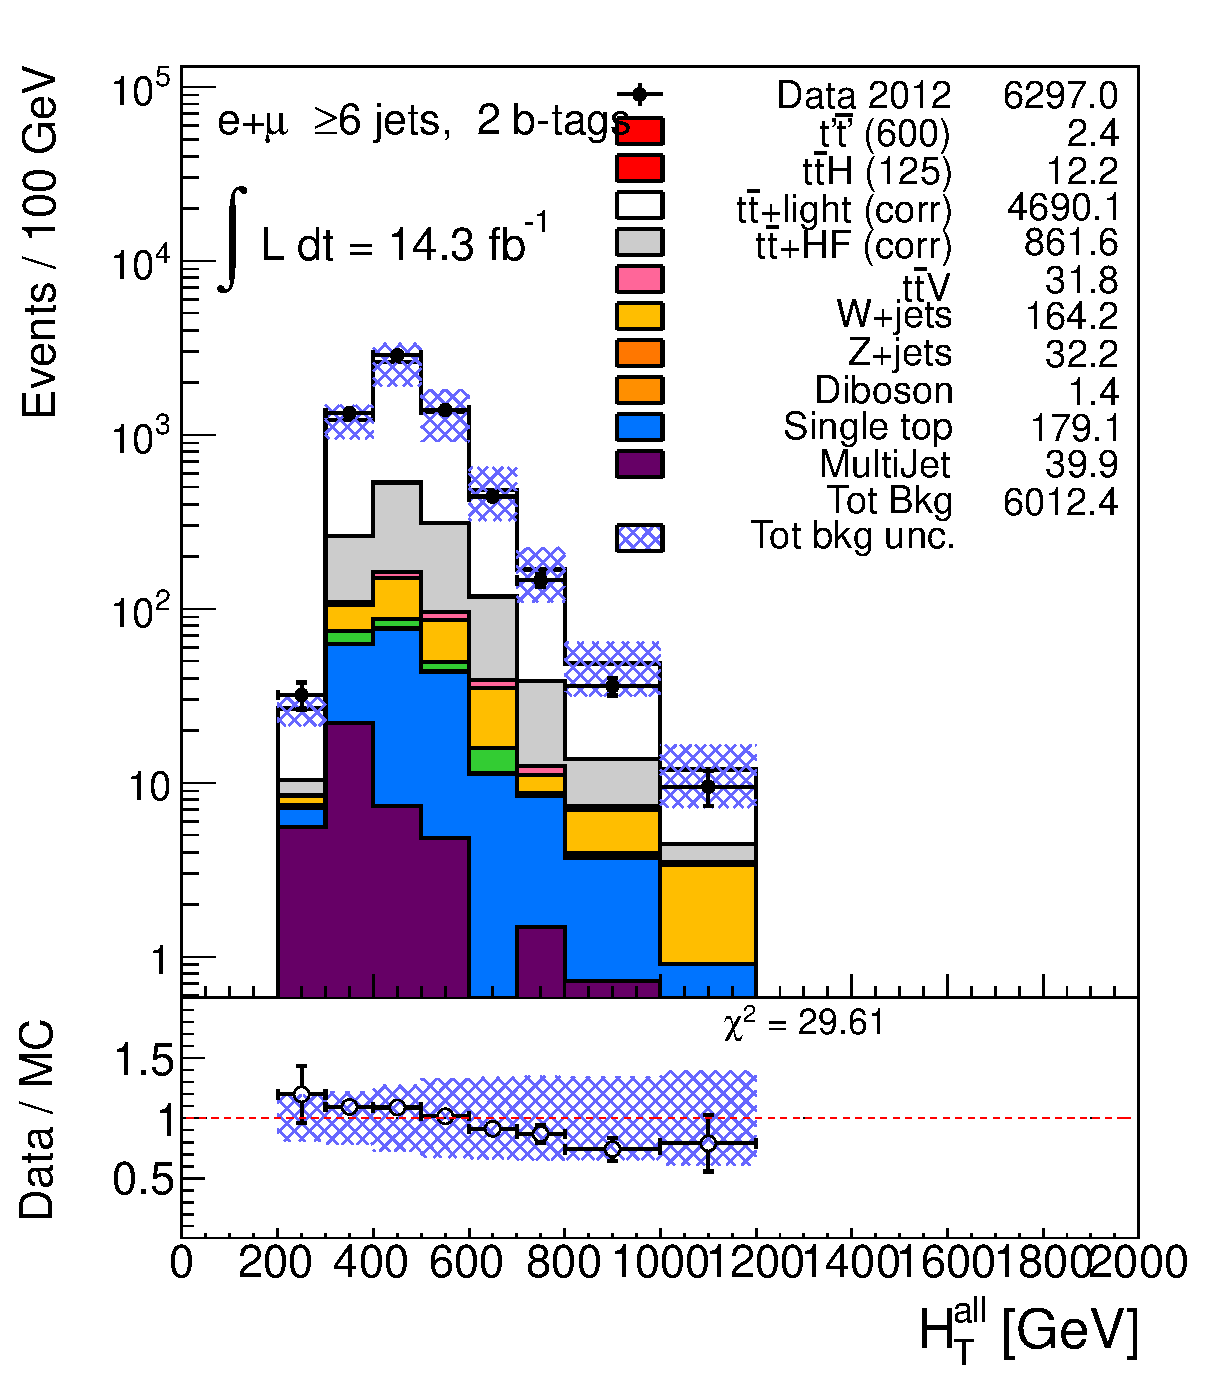
\includegraphics[width=0.4\textwidth]{htx_analysis_14ifb/figures/httails/HTAll_ELEMUON_6jetin2btagex_NOMINAL_logscale.eps}}
	\subfigure[]{\label{fig:httail3}
  	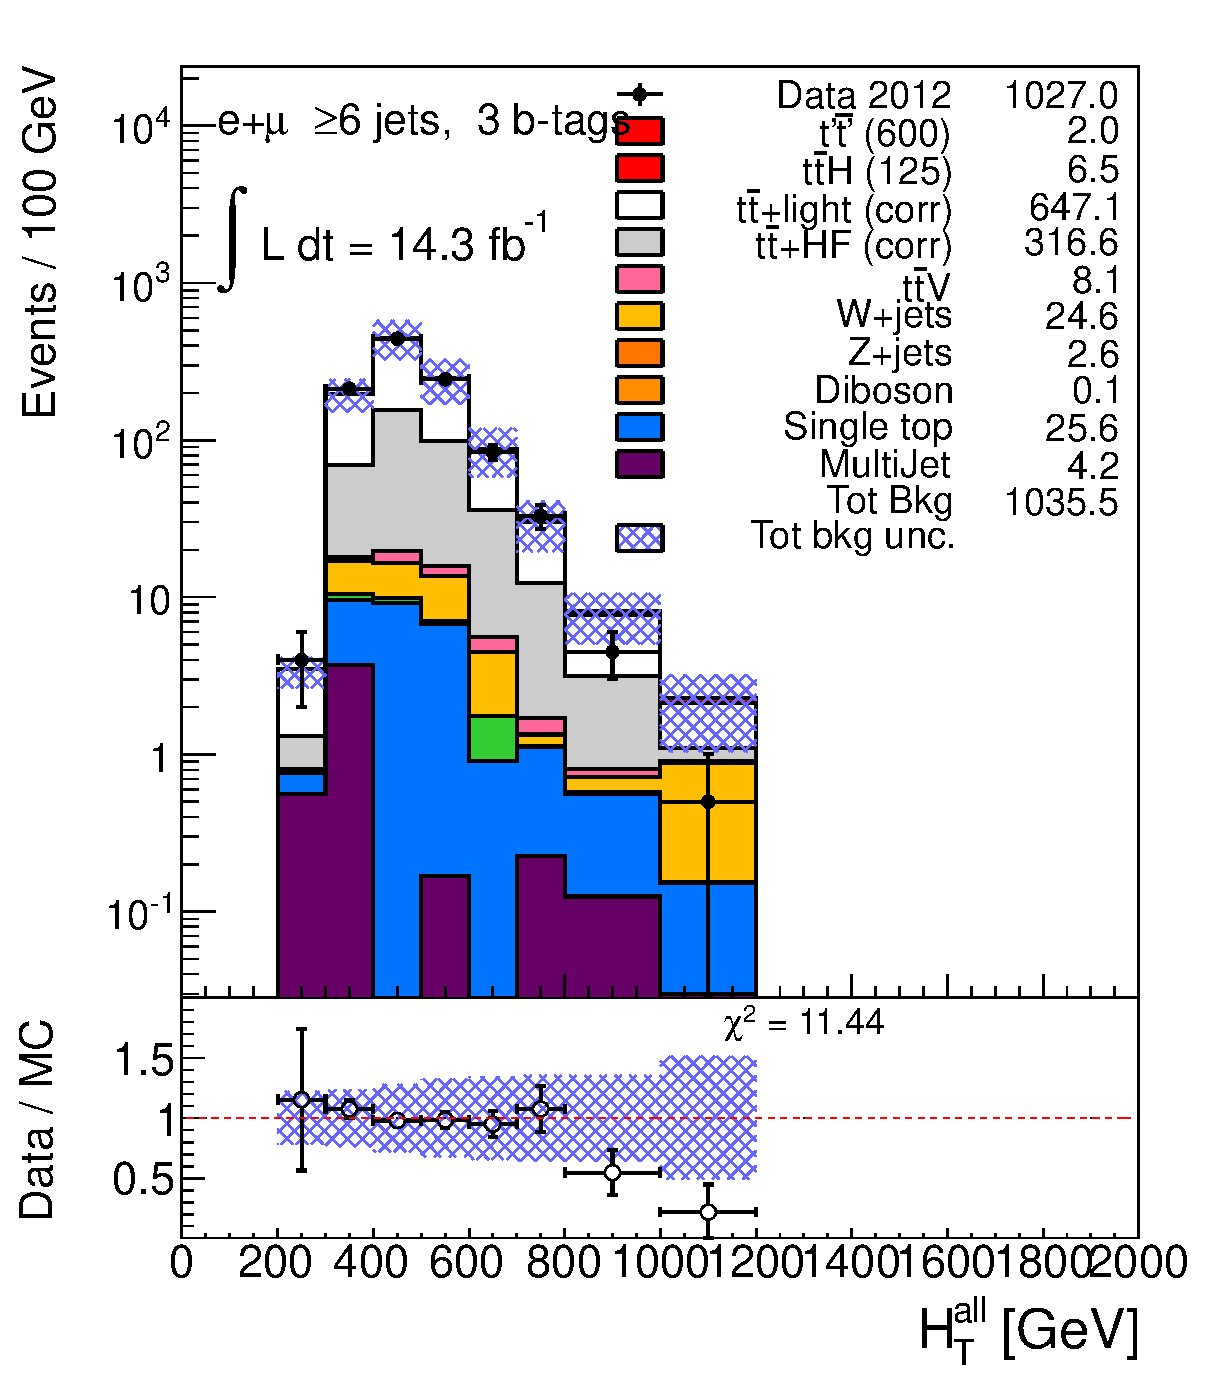
\includegraphics[width=0.4\textwidth]{htx_analysis_14ifb/figures/httails/HTAll_ELEMUON_6jetin3btagex_NOMINAL_logscale.eps}}
	\caption{Comparison between data and simulation for the $\HT$ variable 
        in the combined
        electron and muon channels with $\geq 6$ jets, at most two jets with $\pt>60\gev$,
        $\HT<1.2\tev$ and (a) 2 $b$ tags, and (b) 3 $b$ tags.
        The $t\bar{t}$ background prediction is after fitting to data in the $\HT<700\gev$ region (see text for details).
        Also shown is the expected $\TT$ signal corresponding to $m_{\T}=600\gev$ in the $\T$ doublet scenario.
        The last bin in all figures contains the overflow. The bottom panel displays the ratio between data
        and background prediction. The shaded area represents the total post-fit background uncertainty.  
\label{fig:HT_signalregion_control}}
\end{center}\end{figure}


\section{Final discriminant in the signal region}\label{sec:htxDISCR}


The three search channels, the \chii, \chiii\ and \chiv\ channels,
are now unblinded (except for the \chii, which is kept orthogonal to the
\wbx\ analysis signal region) and the fit to data of the two scaling factors for 
the \tthf\ and \ttlf\ background components is performed over the full range
of the $\HT$ variable.
Consistent values are found with respect to the ones measured 
in the blinded regions, and are $0.88 \pm 0.02\,{\rm (stat.)}$ and 
$1.21 \pm 0.08\,{\rm (stat.)}$ for $t\bar{t}$+light jets 
and $t\bar{t}$+heavy-flavour jets, respectively.  
%A summary of the fitted scaling factors in different configurations can be found in App.~\ref{sec:Fitted_Parameters_Study_Appendix}.
Figure~\ref{fig:HT_SignalRegion} displays the $\HT$ distribution in each of the 
search channels considered, 
showing a large $S/B$ ratio and good discrimination in the \chiv\ channel.
%This figure displays exactly the same data as in Fig.~\ref{fig:HT_beforefit}, except that the blinding cut of $\HT<700\gev$ has
%been removed in the 3 and $\geq 4$ $b$-tag channels.
%The data is found to be consistent with the background prediction and no indications of a signal-like excess is
%observed. Table~\ref{tab:Yields_SignalRegion} summarizes the corresponding event yields in each of the
%analyzed channels.

\begin{figure}[htb]\begin{center}
	\subfigure[]{\label{fig:htall2}
\includegraphics[width=0.30\textwidth]{htx_analysis_14ifb/figures/final/HTAll_6jetin2btagex_ELEMUON.eps}}
	\subfigure[]{\label{fig:htall3}
\includegraphics[width=0.30\textwidth]{htx_analysis_14ifb/figures/final/HTAll_6jetin3btagex_ELEMUON.eps}}
	\subfigure[]{\label{fig:htall4}
\includegraphics[width=0.30\textwidth]{htx_analysis_14ifb/figures/final/HTAll_6jetin4btagin_ELEMUON.eps}}
	\caption{Comparison between data and simulation for $\HT$ in the combined
electron and muon (a) \chii\ (b) \chiii\ and (c) \chiv\ channels.
The $t\bar{t}$ background prediction is after fitting to data using the full $\HT$ spectrum (see text for details).
Also shown is the expected $\TT$ signal corresponding to $m_{\T}=600\gev$ in the $\T$ doublet scenario.
The last bin in all figures contains the overflow. The bottom panel displays the ratio between data
and background prediction. The shaded area represents the total post-fit background uncertainty.
\label{fig:HT_SignalRegion}}
\end{center}\end{figure}


Table~\ref{tab:Yields_SignalRegion} shows the final expected and
observed number of events in the three channels, after applying the rescaling
procedure to the \ttbar\ Monte Carlo simulated sample.

\begin{table}[tb]\centering
\renewcommand{\arraystretch}{1.3}
\begin{tabular}{l*{3}{r@{ $\pm$ }l}}\toprule
 & \multicolumn{2}{c}{$\geq$ 6 jets, 2 $b$-tags} & \multicolumn{2}{c}{$\geq$ 6 jets, 3 $b$-tags} & \multicolumn{2}{c}{$\geq$ 6 jets, $\geq$ 4 $b$-tags}\\
\midrule
$t\bar{t}$+heavy-flavour jets  &  $1500$  &  900 &  $900$  &  400 &  $170$  &  70\\
$t\bar{t}$+light-flavour jets  &  $9600$  &  1000 &  $1900$  &  350 &  $75$  &  22\\
$W$+jets  &  $250$  &  130 &  $50$  &  30 &  $5$  &  3\\
$Z$+jets  &  $50$  &  40 &  $9$  &  6 &  $0.5$  &  0.9\\
Single top  &  $300$  &  70 &  $75$  &  18 &  $7$  &  3\\
Diboson  &  $1.7$  &  0.6 &  $0.3$  &  0.1 &  $0.03$  &  0.03\\
$t\bar{t}V$  &  $70$  &  20 &  $36$  &  12 &  $7$  &  3\\
$t\bar{t}H$  &  $28$  &  4 &  $31$  &  6 &  $12$  &  3\\
Multijet  &  $49$  &  23 &  $1.7$  &  0.8 &  $0.15$  &  0.06\\
\midrule
Total background  &  $11860 $  &  260 &  $2990$  &  210 &  $270$  &  60\\
Data & \multicolumn{2}{c}{$11885$} & \multicolumn{2}{c}{$2922$} & \multicolumn{2}{c}{$318$}\\
\midrule
%\multicolumn{7}{l}{Doublet}\\
%\midrule
$T\bar{T} (600)$ & & & & & & \\
Vector-like doublet &  $4.3$  &  1.2 &  $94$  &  7 &  $79$  &  18\\
Vector-like singlet  &  $2.3$  &  0.4 &  $61$  &  7 &  $36$  &  9\\
%$T\bar{T} (400)$  &  $550$  &  70 &  $1100$  &  100 &  $790$  &  160\\
%$T\bar{T} (600)$  &  $4.3$  &  1.2 &  $94$  &  7 &  $79$  &  18\\
%$T\bar{T} (800)$  &  $0.12$  &  0.05 &  $10.7$  & 0.8 &  $9.1$  &  2.1\\
%\midrule
%\multicolumn{7}{l}{Singlet}\\
%\midrule
%$T\bar{T} (400)$  &  $290$  &  30 &  $650$  &  80 &  $330$  &  70\\
%$T\bar{T} (600)$  &  $2.3$  &  0.4 &  $61$  &  7 &  $36$  &  9\\
%$T\bar{T} (800)$  &  $0.06$  &  0.01 &  $6.9$  &  0.7 &  $4.2$  &  1.1\\
\bottomrule
\end{tabular}


\caption{Predicted and observed yields in the combined 
electron and muon \chii, \chiii\ and \chiv\ channels. 
The $t\bar{t}$ background prediction is after fitting to data 
using the full $\HT$ spectrum (see text for details).
Also shown is the expected $\TT$ signal in both the doublet 
and singlet scenarios for $m_{\T}=600~\gev$. 
The uncertainties shown 
are post-fit and include the effect of 
statistical and systematic uncertainties. 
The uncertainty on the total background is smaller 
than the sum in quadrature of the uncertainties on the individual background
sources due to the anti-correlation between the $t\bar{t}$+light 
jets and $t\bar{t}$+heavy-flavour jets components resulting from 
the fit.\label{tab:Yields_SignalRegion}}
\end{table}

%\section{}\label{sec:}

\section{Systematic uncertainties}\label{sec:htxSYS}

The general aspects of the systematic uncertainties considered
in the \wbx\ and \htx\ analyses were illustrated
in Section~\ref{sec:systematics}, here the traits specific to the
\htx\ analysis will be described.


\subsection{Jet energy scale}\label{sec:htx_syst_jes}
%%JES
As was seen in Table~\ref{tab:SystSummary}, for the \htx\ analysis
the JES systematic uncertainty is split into 8
uncorrelated components, each with a different jet $\pt$ and $\eta$
dependence, which are treated independently.
%The \texttt{JetUncertainties} tool~\cite{jesuncertaintyprovider} allows computation of
%uncertainties corresponding to each of the 8 different eigenvectors.
Looking at the effects of the individual sources of systematic uncertainty, 
it is evident that the dominant contribution comes from the first 
eigenvector (``BASELINE''), while the rest of the
eigenvectors lead in general to very small systematic uncertainties, 
except for those Monte Carlo samples characterized by low statistics
in the final selection channels, where unphysical fluctuations
can lead to artificially large uncertainties. 
%Given the limited MC statistics available for the leading backgrounds,
%we are currently considering the JES envelope uncertainty (i.e. no JES breakdown)
%in order to attempt to get a physical estimate of the uncertainty in the analysis.
%We believe this actually provides a more accurate assessment of the JES uncertainty
%in this analysis, although we are likely still double-counting statistical uncertainties from the MC.

\subsection{Normalization of backgrounds}\label{sec:syst_normHTX}

The $W$/$Z$+jets cross sections as computed at the
leading-order in the
\texttt{Alpgen} generator framework
are affected by large uncertainties.
It was explained in Section~\ref{sec:Wjetsnorm}
that the overall $W$+jets normalization is 
corrected using data-driven methods 
performing the estimation in each jet multiplicity
separately for events with exactly 4 and $\geq 5$ 
jets in order to ensure the best possible central value for the 
predicted $W$+jets yield. 
An additional 24\% uncertainty is assigned to the extrapolation of the data driven
estimate to events with $\geq 6$ jets.
%The first two uncertainties result from the propagation of the experimental uncertainties in the
%measurement of the heavy-flavour fractions in $W$+1 jet and $W$+2 jets data control samples.
Additional normalization uncertainties are evaluated by varying 
the fractions of heavy- and light-flavor components of the $W$+jets background
in different ways and by studying the $W$+heavy-flavour fractions as
a function of \texttt{Alpgen} paramteters,
as explained in~\cite{topcommon2013}.
The sum in quadrature of all the above contributions result in a 
total uncertainty of $\sim$50\% on
the estimated $W$+jets normalisation for events 
with $\geq 6$ jets and $\geq 2$ $b$ tagged jets. 
The same uncertainty is also assigned to the $Z$+jets normalisation.

Systematic uncertainties on the QCD multijet background 
estimate via the Matrix Method receive
contributions from the limited data statistics, 
particularly at high jet and $b$-tag multiplicities, as
well as from the uncertainty on the method, based on 
the difference between estimates obtained using 
different control regions and from the calibration 
of the method using simulated QCD multijet events.
The uncertainty due to the method is assessed to be 
50\%, which is taken as correlated across jet
and $b$-tag multiplicity bins. 
%The statistical uncertainties in the channels with 4 jets
%are only a few percent and are therefore neglected.
%The statistical uncertainties in the channels with 5 jets and 6 jets 
% are in the range of 10\%--54\% and 
%14\%--66\%, respectively, depending on the $b$-tag multiplicity bin.
%These uncertainties are treated as uncorrelated across jet and $b$-tag multiplicity bins.




\subsection{$t\bar{t}$+jets Modelling}
\label{sec:syst_ttbarmodelHTX}

A number of systematic uncertainties affecting 
the modelling of $t\bar{t}$+jets are considered
in this analysis. Systematic uncertainties associated 
with the choice of factorisation and renormalisation 
scales in {\sc Alpgen} are considered. For the former, 
two different uncertainties are taken into account.
\subsubsection*{$\mathbf{Q_{fac}}$}
The factorisation scale for the hard scatter is varied by a factor of two up and down relative to the
original scale, $Q^2=\sum_{\rm partons} (m^2 + \pt^2)$.
\ifIsINT 
Appendix~\ref{app:AlpgenModellingAppendix} describes details of the
implementations of this uncertainty for the $t\bar{t}$+light partons and $t\bar{t}Q\bar{Q}$ ($Q=b,c$) samples, which are different.
\fi
Since sometimes both variations can go in the same direction, the largest of the two is taken and symmetrised.

\subsubsection*{Functional form of the factorisation scale (iqopt2)} 
On the other hand, the default choice for the dynamic factorisation scale,
$Q^2=\sum_{\rm partons} (m^2 + \pt^2)$,  is compared to an alternate choice, $Q^2=x_1 x_2 s$.
\ifIsINT
See Appendix~\ref{app:AlpgenModellingAppendix} for more details on the implementations of this uncertainty 
for the $t\bar{t}$+light jets and $t\bar{t}Q\bar{Q}$ ($Q=b,c$) samples, which are different).
\fi
This uncertainty is significantly larger than that obtained by simply scaling the factorization scale up and down by a factor two 
and is symmetrised to obtain a two-sided uncertainty.

\subsubsection*{$\mathbf{k_{Tfac}}$}
The renormalisation scale associated with the evaluation of $\alpha_s$ at each local
vertex in the matrix element calculation is varied by a factor of two
up and down relative to the original scale, $k_{\rm T}$, between two
partons.  
\ifIsINT 
Additional details are described in Appendix~\ref{app:AlpgenModellingAppendix}.
\fi 
This uncertainty is only applicable for the $t\bar{t}$+light partons
sample, since that is the only sample to which the MLM matching prescription~\cite{mlm} is
applied. As a result, this uncertainty cannot be applied to the events 
originating from the dedicated $t\bar{t}b\bar{b}$ and $t\bar{t}c\bar{c}$
simulated samples. However, this uncertainty is applied to the subset of $t\bar{t}b\bar{b}$ and $t\bar{t}c\bar{c}$
events selected from the $t\bar{t}$+light partons MC samples after the
heavy-flavour overlap removal procedure.

%\paragraph{Heavy-flavour overlap removal}:  The $\Delta R$ cut between $Q\bar{Q}$ pairs in $t\bar{t}Q\bar{Q}$ ($Q=b,c$)  used to decide
%whether to take the matrix element or parton shower predictions is varied by $\pm 0.1$ about the nominal value
%of $\Delta R=0.4$. {\em Caveat: this systematic uncertainty has not been incorporated in the analysis yet.}

\subsection{$t\bar{t}$+jets Heavy-Flavour Content}
\label{sec:syst_ttbarHF}
The fraction of $t\bar{t}Q\bar{Q}$ ($Q=b,c$) events relative to all $t\bar{t}jj$ events, where $j$ denotes any parton,
is one of the most important systematic uncertainties in this analysis. 
Currently there are no available theoretical predictions for the $t\bar{t}$+heavy-flavour fractions in $pp$ collisions at $\sqrt{s}=8\tev$ at NLO matched to a parton shower.
In order to estimate a systematic uncertainty, the dependence of the ratio of cross sections for $t\bar{t}b\bar{b}$ over
$t\bar{t}jj$ as a function of the factorisation scale choice is examined in {\sc Alpgen}. These cross
sections are computed requiring the extra partons to satisfy $\pt>20\gev$, $|\eta|<2.5$ and $\Delta R({\rm j},{\rm j})>0.4$, which are similar requirements
to those used in this analysis. The ratio of cross sections is computed for the default factorisation scale choice
in {\sc Alpgen}, $Q^2=\sum_{\rm partons} (m^2 + \pt^2)$, which is then scaled up and down by a factor of two
in a correlated way for $t\bar{t}b\bar{b}$ and $t\bar{t}jj$.
The variation in the ratio of cross sections is found to be $\leq 25\%$. A similar conclusion is reached if a
different dynamic scale,  $Q^2=x_1 x_2 s$, is chosen, and then scaled up and down by a factor of two.
The systematic uncertainty assigned to the $t\bar{t}$+heavy-flavour fraction is 50\%, conservatively doubling
the variation found in the generator-level study with {\sc Alpgen}. 

Therefore, the fraction of $t\bar{t}Q\bar{Q}$ ($Q=b,c$) events relative to all $t\bar{t}$+jets events
is varied up and down by $\pm 50\%$ (relative) with respect to the original {\sc Alpgen} prediction. 
This uncertainty is taken to be fully correlated between the $t\bar{t}b\bar{b}$ and $t\bar{t}c\bar{c}$ fractions.
The fraction of $t\bar{t}$+light jet events is adjusted accordingly to preserve the total $t\bar{t}$ yield in each jet multiplicity bin 
prior to any $b$-tagging requirement.


\subsection{\tthf\ and \ttlf\ yields}\label{sec:htxNuisance}

Since the prediction for the $t\bar{t}$ background
in the \chiv\ channel (the most sensitive one) is affected by large
systematic uncertainties originating from \bjet\ identification, jet energy calibration and
physics modelling, including the fraction of $t\bar{t}$+heavy-flavour jets, 
two nuisance parameters are introduced.
These parameters correspond to  scaling factors on the overall yields of 
\tthf\ and \ttlf, and by allowing them to be fitted to data during the statistical analysis
particularly in the \chii\ and \chiii\ channels dominated by background,
the degrading impact of systematic uncertainties on the sensitivity of the search
is significantly reduced. 

\subsection{Overall effect of systematic uncertainties}\label{sec:htxALLSYS}

In Table~\ref{tab:htxSYS4b} the final results on
the effect of the different systematic uncertainties affecting
the \htx\ analysis are reported.
The overall systematic uncertainty in the \chiv\ channel
before the two-parameter fit ({\it pre-fit})
on the background normalization was
$\sim$42\%, with the dominant uncertainties being from $b$ tagging efficiency (16\%),
$c$ tagging efficiency (11\%), jet energy scale (11\%), $t\bar{t}$ modelling (11\%), 
$t\bar{t}$+heavy-flavour fractions (32\%) and $t\bar{t}$ cross section (10\%).
As a result of the two-parameter fit, the total background uncertainty 
in this channel is reduced 
by about 80\%. The total  systematic uncertainty
in the signal normalisation in the $\geq 4$ $b$-tags channel is 
$\sim$21\%, completely dominated by the uncertainty in the $b$ tagging efficiency.


\begin{table}[h!tb]
\begin{center}
\resizebox{1.\textwidth}{!}{
\begin{tabular}{l*{10}{c}}
\toprule
\multicolumn{11}{c}{$\geq$ 6 jets, $\geq$ 4 $b$-tags}\\
\midrule
 & vlt & $t\bar{t}$H (125) & $t\bar{t}$-HF & $t\bar{t}$-Light & $W$+jets & $Z$+jets & Single top & Diboson & $t\bar{t}$$V$ & Multijet\\
\midrule
BTAGBREAK0 & +0.0/-0.0 & +0.2/-0.2 & +0.0/-0.0 & +0.1/-0.1 & +0.1/-0.0 & +1.0/-1.0 & +0.1/-0.1 & +0.3/-0.3 & +0.1/-0.1 & --\\
BTAGBREAK1 & +0.7/-0.7 & +0.5/-0.5 & +0.5/-0.5 & +0.3/-0.3 & +0.1/-0.0 & +0.2/-0.2 & +1.1/-1.2 & +2.8/-2.8 & +0.4/-0.4 & --\\
BTAGBREAK2 & +0.4/-0.4 & +0.2/-0.2 & +0.1/-0.1 & +0.1/-0.1 & +0.5/-0.5 & +0.8/-0.8 & +0.2/-0.2 & +2.4/-2.4 & +0.2/-0.2 & --\\
BTAGBREAK3 & +0.9/-0.9 & +0.3/-0.3 & +0.2/-0.2 & +0.3/-0.3 & +0.5/-0.5 & +0.2/-0.1 & +0.1/-0.1 & +1.9/-1.8 & +0.1/-0.1 & --\\
BTAGBREAK4 & +1.4/-1.4 & +1.8/-1.8 & +1.6/-1.6 & +1.5/-1.5 & +0.3/-0.3 & +0.1/-0.1 & +1.0/-1.0 & +1.8/-1.7 & +1.3/-1.3 & --\\
BTAGBREAK5 & +2.7/-2.7 & +1.4/-1.4 & +1.0/-1.0 & +0.7/-0.7 & +0.4/-0.4 & +2.1/-2.1 & +1.7/-1.7 & +0.9/-0.6 & +1.2/-1.2 & --\\
BTAGBREAK6 & +1.0/-1.0 & +0.7/-0.7 & +0.7/-0.8 & +0.5/-0.5 & +1.5/-1.5 & +1.4/-1.4 & +0.7/-0.7 & +1.3/-1.2 & +0.7/-0.7 & --\\
BTAGBREAK7 & +0.1/-0.1 & +4.1/-4.2 & +4.1/-4.3 & +3.4/-3.5 & +5.5/-5.6 & +1.1/-1.1 & +4.4/-4.7 & +0.5/-0.3 & +3.4/-3.5 & --\\
BTAGBREAK8 & +20.4/-22.7 & +18.7/-21.6 & +15.8/-17.8 & +12.2/-13.1 & +13.5/-15.0 & +13.0/-13.9 & +15.9/-17.8 & +22.0/-27.4 & +16.4/-18.6 & --\\
CTAGBREAK0 & +0.3/-0.3 & +0.3/-0.3 & +0.9/-0.9 & +1.2/-1.2 & +1.5/-1.6 & +0.8/-0.8 & +1.1/-1.1 & +0.4/-0.5 & +0.6/-0.6 & --\\
CTAGBREAK1 & +0.0/-0.0 & +0.2/-0.2 & +0.7/-0.7 & +1.0/-1.0 & +0.2/-0.3 & +2.7/-2.8 & +0.6/-0.6 & +0.0/-0.0 & +0.5/-0.5 & --\\
CTAGBREAK2 & +0.1/-0.1 & +0.2/-0.2 & +0.5/-0.5 & +0.6/-0.6 & +1.7/-1.7 & +2.6/-2.7 & +0.5/-0.5 & +0.4/-0.4 & +0.5/-0.5 & --\\
CTAGBREAK3 & +1.5/-1.5 & +1.9/-2.0 & +5.0/-5.2 & +5.3/-5.4 & +6.2/-6.6 & +6.1/-6.2 & +3.8/-3.9 & +2.7/-2.9 & +4.8/-5.0 & --\\
CTAGBREAK4 & +2.4/-2.4 & +3.5/-3.6 & +9.4/-10.1 & +10.2/-10.5 & +11.8/-13.8 & +16.5/-18.3 & +8.3/-8.8 & +3.8/-4.3 & +8.5/-9.1 & --\\
Dibosons XS & -- & -- & -- & -- & -- & -- & -- & +5.0/-5.0 & -- & --\\
JER & +0.9/-0.9 & +0.5/-0.5 & +1.9/-1.9 & +4.3/-4.3 & +7.9/-7.9 & +21.9/-21.9 & +9.6/-9.6 & +63.2/-63.2 & +0.6/-0.6 & --\\
JESBREAK1 & +3.1/-3.1 & +7.3/-7.3 & +10.5/-10.5 & +13.7/-13.7 & +18.1/-18.1 & +18.2/-18.2 & +19.9/-19.9 & +5.2/-5.2 & +8.4/-8.4 & --\\
JESBREAK2 & +0.7/-0.7 & +1.8/-1.8 & +3.1/-3.1 & +3.4/-3.4 & +7.2/-7.2 & +0.4/-0.4 & +2.9/-2.9 & +0.2/-0.2 & +1.9/-1.9 & --\\
JESBREAK3 & +0.0/-0.0 & +0.7/-0.7 & +0.9/-0.9 & +1.2/-1.2 & +6.6/-6.6 & +10.8/-10.8 & +1.4/-1.4 & +0.3/-0.3 & +0.7/-0.7 & --\\
JESBREAK4 & +0.3/-0.3 & +0.2/-0.2 & +0.6/-0.6 & +0.7/-0.7 & +0.8/-0.8 & +11.1/-11.1 & +2.0/-2.0 & +0.6/-0.6 & +0.4/-0.4 & --\\
JESBREAK5 & +0.1/-0.1 & +1.6/-1.6 & +2.2/-2.2 & +2.7/-2.7 & +8.7/-8.7 & +1.0/-1.0 & +2.3/-2.3 & +0.7/-0.7 & +1.8/-1.8 & --\\
JESBREAK6 & +0.7/-0.7 & +2.0/-2.0 & +4.0/-4.0 & +7.0/-7.0 & +0.2/-0.2 & +0.2/-0.2 & +2.6/-2.6 & +0.7/-0.7 & +3.1/-3.1 & --\\
JESBREAK7 & +0.2/-0.2 & +1.1/-1.1 & +2.2/-2.2 & +4.0/-4.0 & +1.5/-1.5 & +1.9/-1.9 & +0.8/-0.8 & +0.1/-0.1 & +1.7/-1.7 & --\\
JESBREAK8 & +1.2/-1.2 & +3.2/-3.2 & +3.5/-3.5 & +2.7/-2.7 & +8.9/-8.9 & +1.3/-1.3 & +5.8/-5.8 & +0.8/-0.8 & +2.9/-2.9 & --\\
JVFSF & +3.0/-3.0 & +2.1/-2.8 & +1.9/-2.7 & +2.0/-2.9 & +1.7/-2.3 & +2.2/-2.7 & +2.3/-3.3 & +1.9/-1.8 & +2.1/-2.7 & --\\
LEPTONSYS & +2.1/-2.1 & +2.1/-2.1 & +2.1/-2.1 & +2.1/-2.1 & +2.1/-2.1 & +1.5/-1.5 & +2.1/-2.1 & +2.1/-2.1 & +2.1/-2.1 & --\\
LTAG & +1.7/-1.8 & +1.6/-1.6 & +3.1/-3.2 & +16.8/-17.7 & +6.8/-7.3 & +13.4/-14.5 & +6.7/-7.0 & +6.9/-7.4 & +3.3/-3.3 & --\\
Luminosity & +3.6/-3.6 & +3.6/-3.6 & +3.6/-3.6 & +3.6/-3.6 & +3.6/-3.6 & +3.6/-3.6 & +3.6/-3.6 & +3.6/-3.6 & +3.6/-3.6 & --\\
QCD norm & -- & -- & -- & -- & -- & -- & -- & -- & -- & +50.0/-50.0\\
Vjets XS jet6 & -- & -- & -- & -- & +50.0/-50.0 & +50.0/-50.0 & -- & -- & -- & --\\
ttbar iqopt2 & -- & -- & +6.9/-6.9 & +20.1/-20.1 & -- & -- & -- & -- & -- & --\\
ttbar ktfac & -- & -- & +7.5/-9.2 & +13.8/-17.0 & -- & -- & -- & -- & -- & --\\
ttbar qfac & -- & -- & +0.7/-0.7 & +1.6/-1.6 & -- & -- & -- & -- & -- & --\\
singleTop XS & -- & -- & -- & -- & -- & -- & +4.7/-3.7 & -- & -- & --\\
ttH125 XS & -- & +12.0/-17.0 & -- & -- & -- & -- & -- & -- & -- & --\\
ttbarHF & -- & -- & +50.0/-50.0 & +13.0/-13.0 & -- & -- & -- & -- & -- & --\\
ttbarV XS & -- & -- & -- & -- & -- & -- & -- & -- & +30.0/-30.0 & --\\
ttbar XS & -- & -- & +9.9/-10.7 & +9.9/-10.7 & -- & -- & -- & -- & -- & --\\
\midrule
Total & +21.9/-24.0 & +25.2/-30.0 & +57.3/-58.4 & +42.0/-44.1 & +60.0/-61.0 & +65.2/-66.2 & +31.7/-32.9 & +68.2/-70.2 & +37.6/-38.8 & +50.0/-50.0\\
\bottomrule
\end{tabular}
}
\caption{List of all systematic uncertainties (in \%) considered in the analysis, indicating which ones are treated
as normalisation and/or shape uncertainties, with their impact on normalisation in the case of the 
\chiv\ channel, for signal and backgrounds. \label{tab:htxSYS4b} }
\end{center}
\end{table}



\subsection{Impact of profiling}\label{sec:fullprof}

%\section{Cross-Check of Background Prediction Using Full Profiling}
%\label{sec:FullProfiling_Study_Appendix}

%As explained in Section~\ref{sec:htxEVT}, t
The final background 
prediction in the signal region is obtained by fitting two overall
normalization parameters, one for $t\bar{t}$+light jets 
and another for $t\bar{t}$+heavy-flavor jets, to the $\HT$ distribution in the
three analysis channels \chii, \chiii\ and \chiv. 
This simplified background 
calibration may not be sufficient to obtain an accurate 
(both in terms of normalization and shape) 
modeling of the background in the most sensitive channel, the
\chiv\ channel.
In particular, a potential slope in the data to Monte Carlo 
ratio versus $\HT$ would not be corrected for by the 
simple two-parameter fit.

Here we study the predicted background by performing 
a fit to data considering all nuisance parameters 
(a total of 38) describing fundamental
sources of uncertainty in the analysis (referred to as 
``full profiling''). This allows 
to correct for potential mismodelings in the 
background-dominated channels
and port those corrections in a physical way 
into the signal region. 
To be consistent, the nominal $t\bar{t}$ \texttt{ALPGEN} 
prediction, rather than the scaled one, is used.

The results obtained, detailed in Appendix~\ref{app:fullprofiling},
give that most nuisance parameters are well within
$1\sigma$ of their a-priori value (zero) and almost 
not constrained with respect to their a-priori error (one). 
%Prefit & Postfit (full profiling) & Postfit (two-parameter fit) \\
Figure~\ref{fig:HT_SignalRegion_FullProfiling} compares, 
for each of the three analysis channels, the $\HT$ distribution 
prefit and postfit from the fit using full profiling, and with 
the postfit distribution
obtained from the two-parameter fit. As it can be appreciated, 
the full profiling achieves the desired effect of correcting 
the shape of the $\HT$ 
distribution in the low $b$-tag multiplicity channels. However, 
in the $\geq 4$ $b$-tags channel both post-fit predictions still look quite similar,
which gives confidence in the simplified fit procedure.
The corresponding postfit yields after full profiling are 
compared to the yields from the two-parameter fit in
 Appendix~\ref{app:fullprofiling}, and the total background predictions 
in the \chiv\ channel are found to be in agreement within $\sim 10\%$.

\begin{figure}[h!tb]\begin{center}
\begin{minipage}{0.27\textwidth}
\centering
Prefit
\end{minipage}\begin{minipage}{0.27\textwidth}
\centering
Postfit\\ (full profiling)
\end{minipage}
\begin{minipage}{0.27\textwidth}
\centering
Postfit\\ (two-parameters fit)
\end{minipage}
	\subfigure[]{
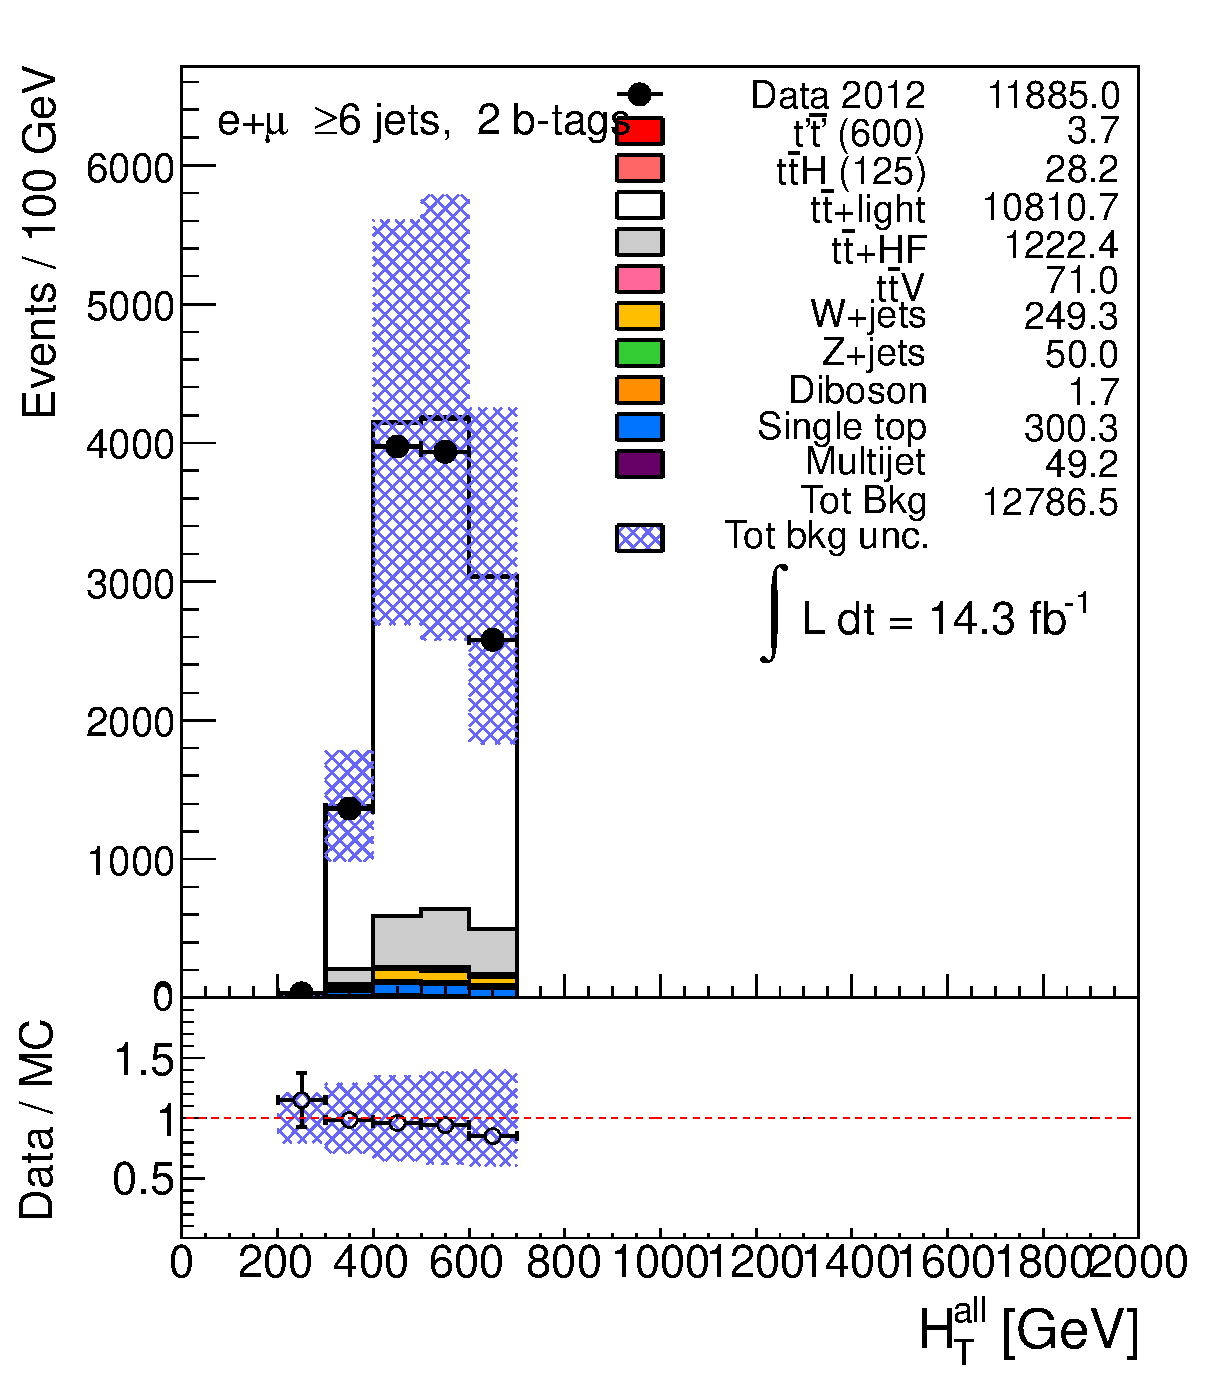
\includegraphics[width=0.27\textwidth]{htx_analysis_14ifb/figures/fullprof/Prefit/HTAll_6jetin2btagex_ELEMUON.eps}}
	\subfigure[]{
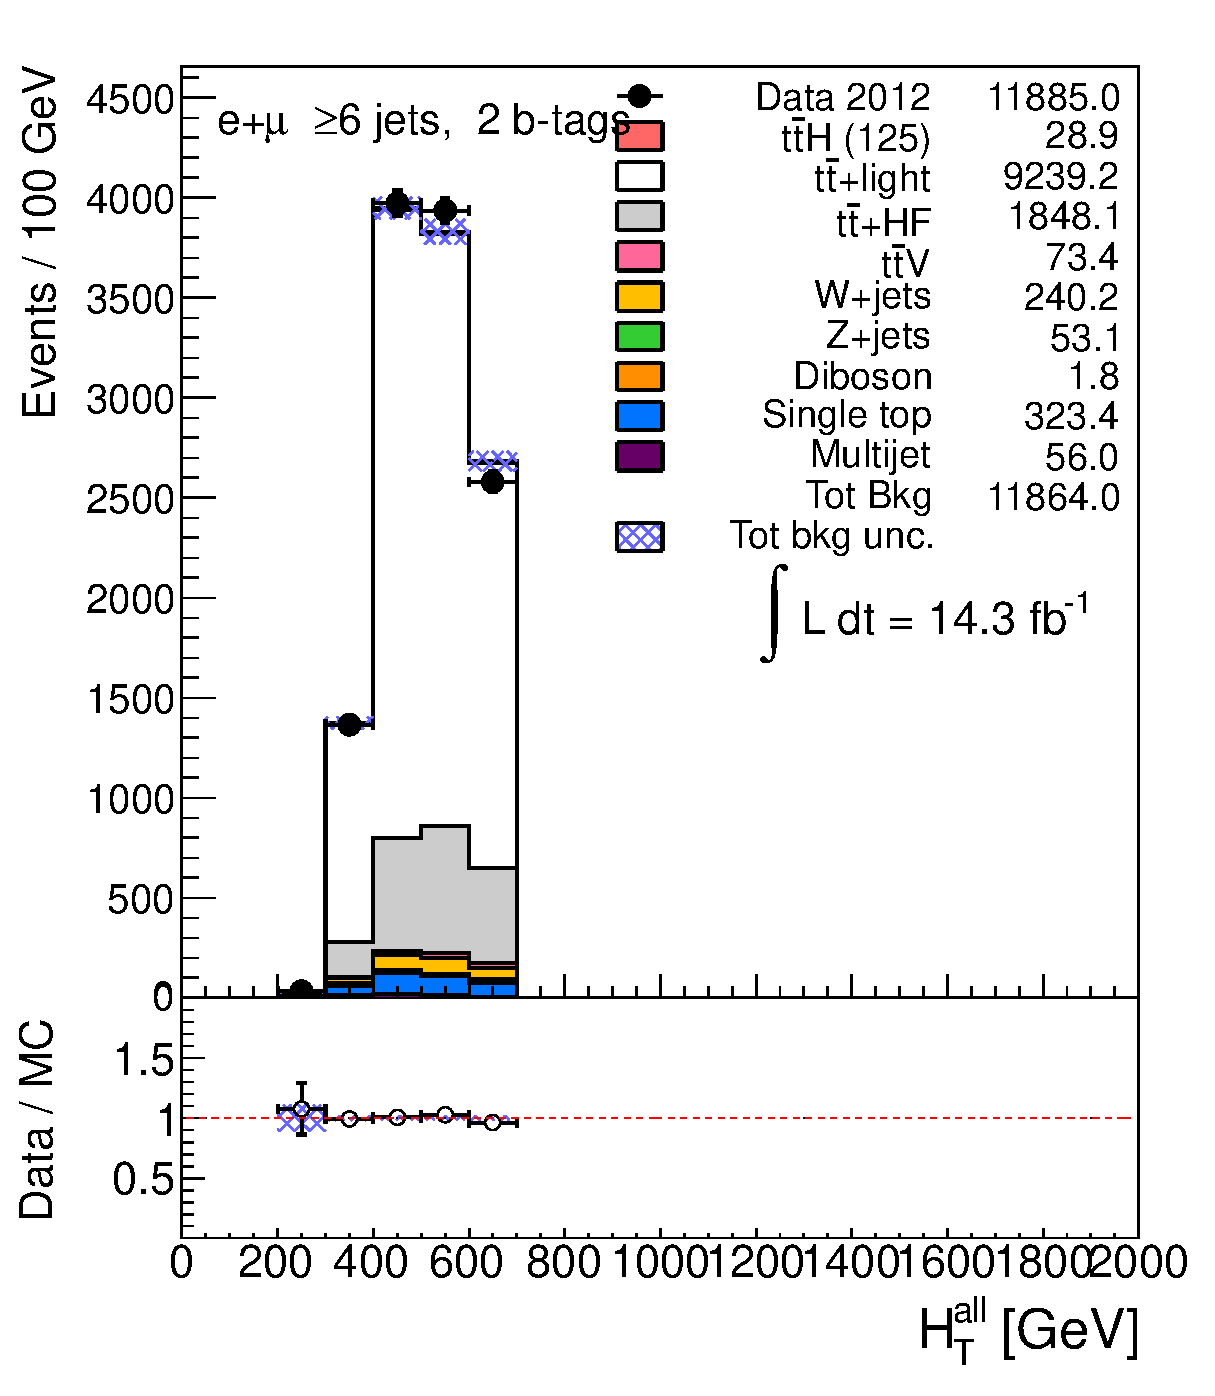
\includegraphics[width=0.27\textwidth]{htx_analysis_14ifb/figures/fullprof/PostFit_null/HTAll_6jetin2btagex_ELEMUON.eps}}
	\subfigure[]{
\includegraphics[width=0.27\textwidth]{htx_analysis_14ifb/figures/fullprof/sysband_Postfit_null/HTAll_6jetin2btagex_ELEMUON.eps}} \\
	\subfigure[]{
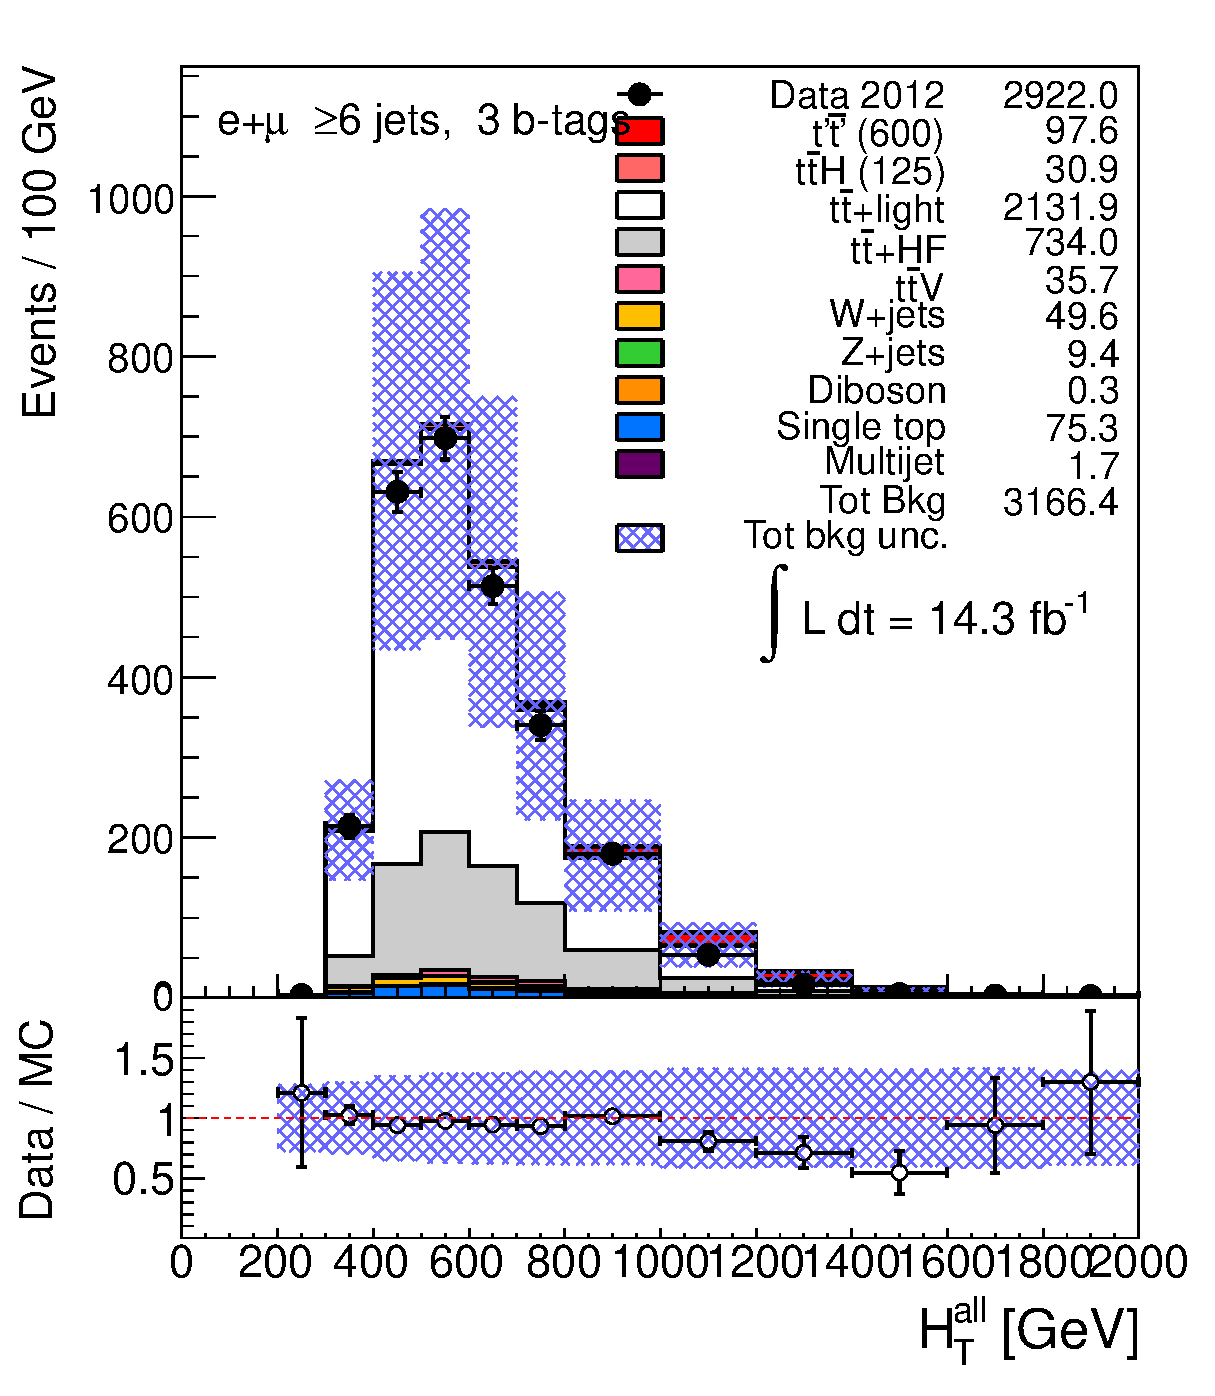
\includegraphics[width=0.27\textwidth]{htx_analysis_14ifb/figures/fullprof/Prefit/HTAll_6jetin3btagex_ELEMUON.eps}}
	\subfigure[]{
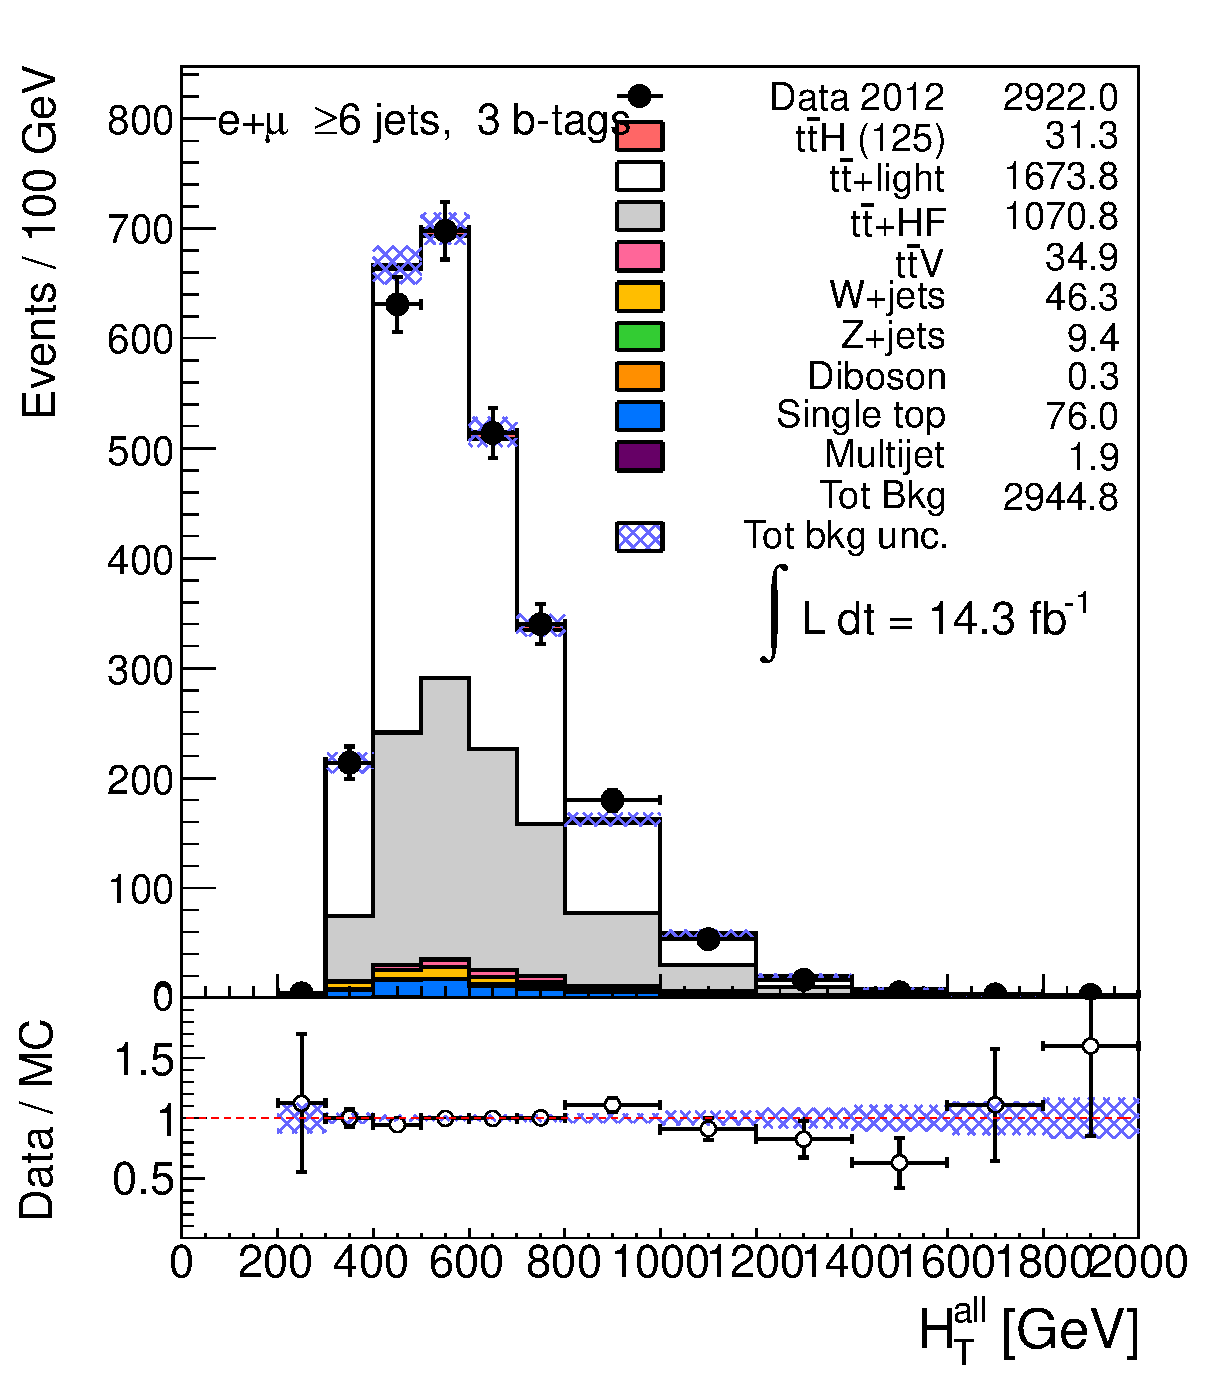
\includegraphics[width=0.27\textwidth]{htx_analysis_14ifb/figures/fullprof/PostFit_null/HTAll_6jetin3btagex_ELEMUON.eps}}
	\subfigure[]{
\includegraphics[width=0.27\textwidth]{htx_analysis_14ifb/figures/fullprof/sysband_Postfit_null/HTAll_6jetin3btagex_ELEMUON.eps}} \\
	\subfigure[]{
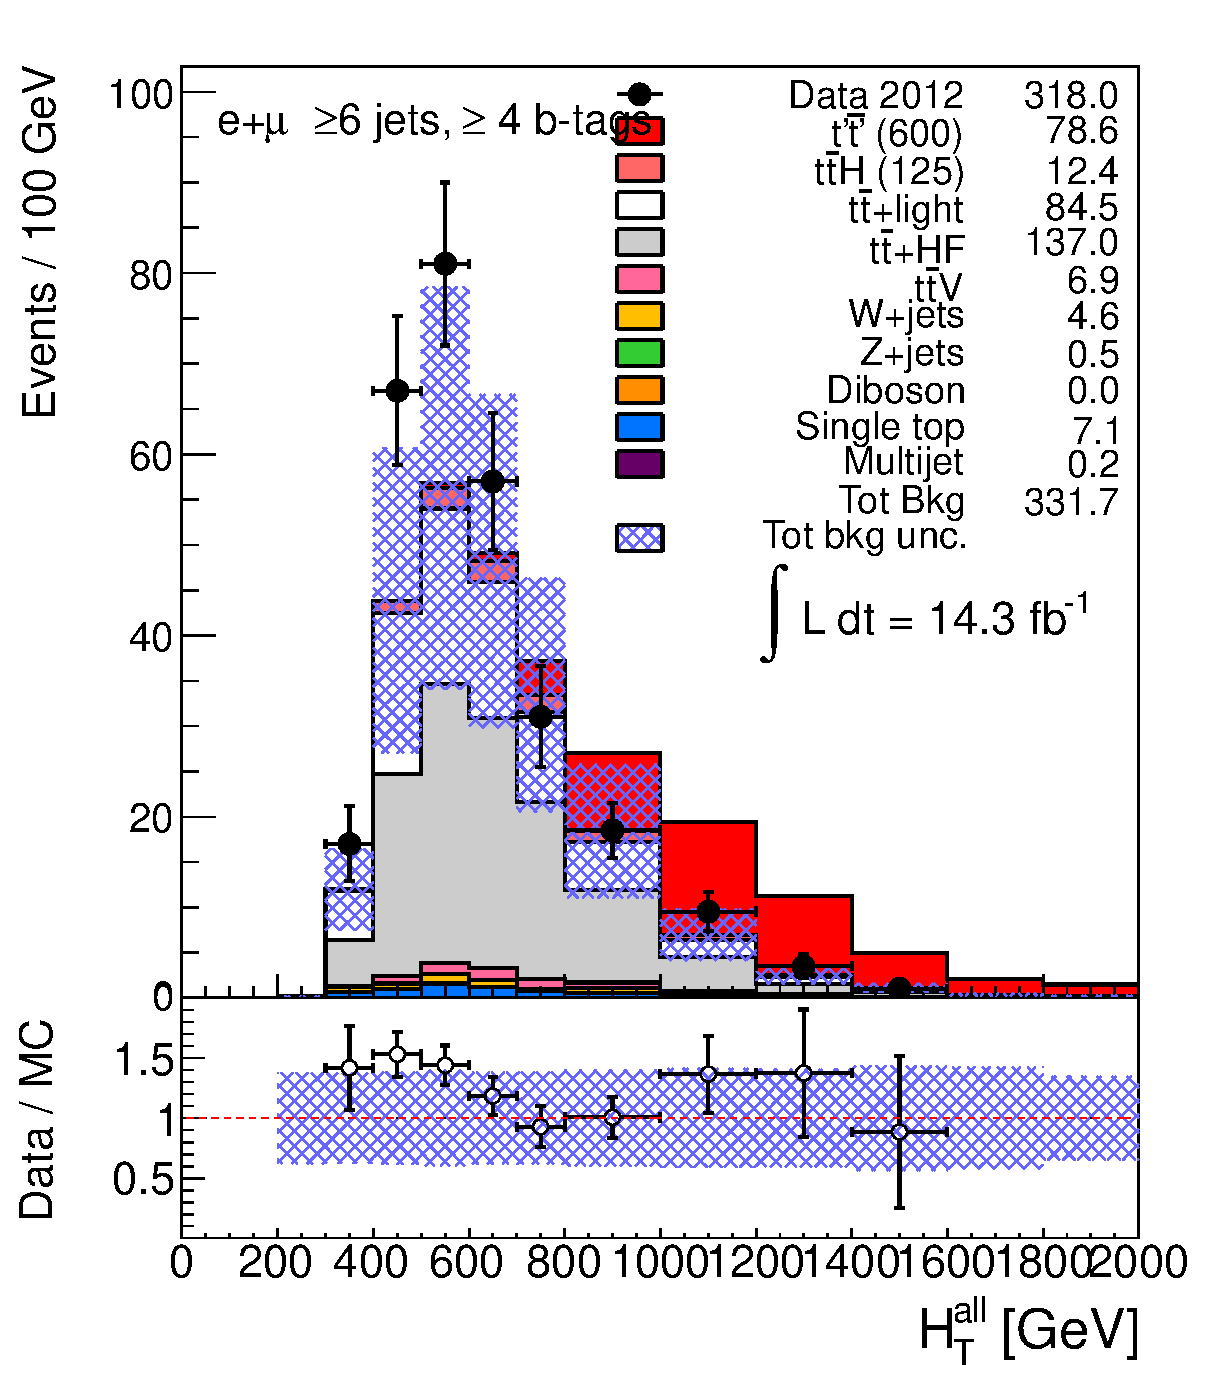
\includegraphics[width=0.27\textwidth]{htx_analysis_14ifb/figures/fullprof/Prefit/HTAll_6jetin4btagin_ELEMUON.eps}}
	\subfigure[]{
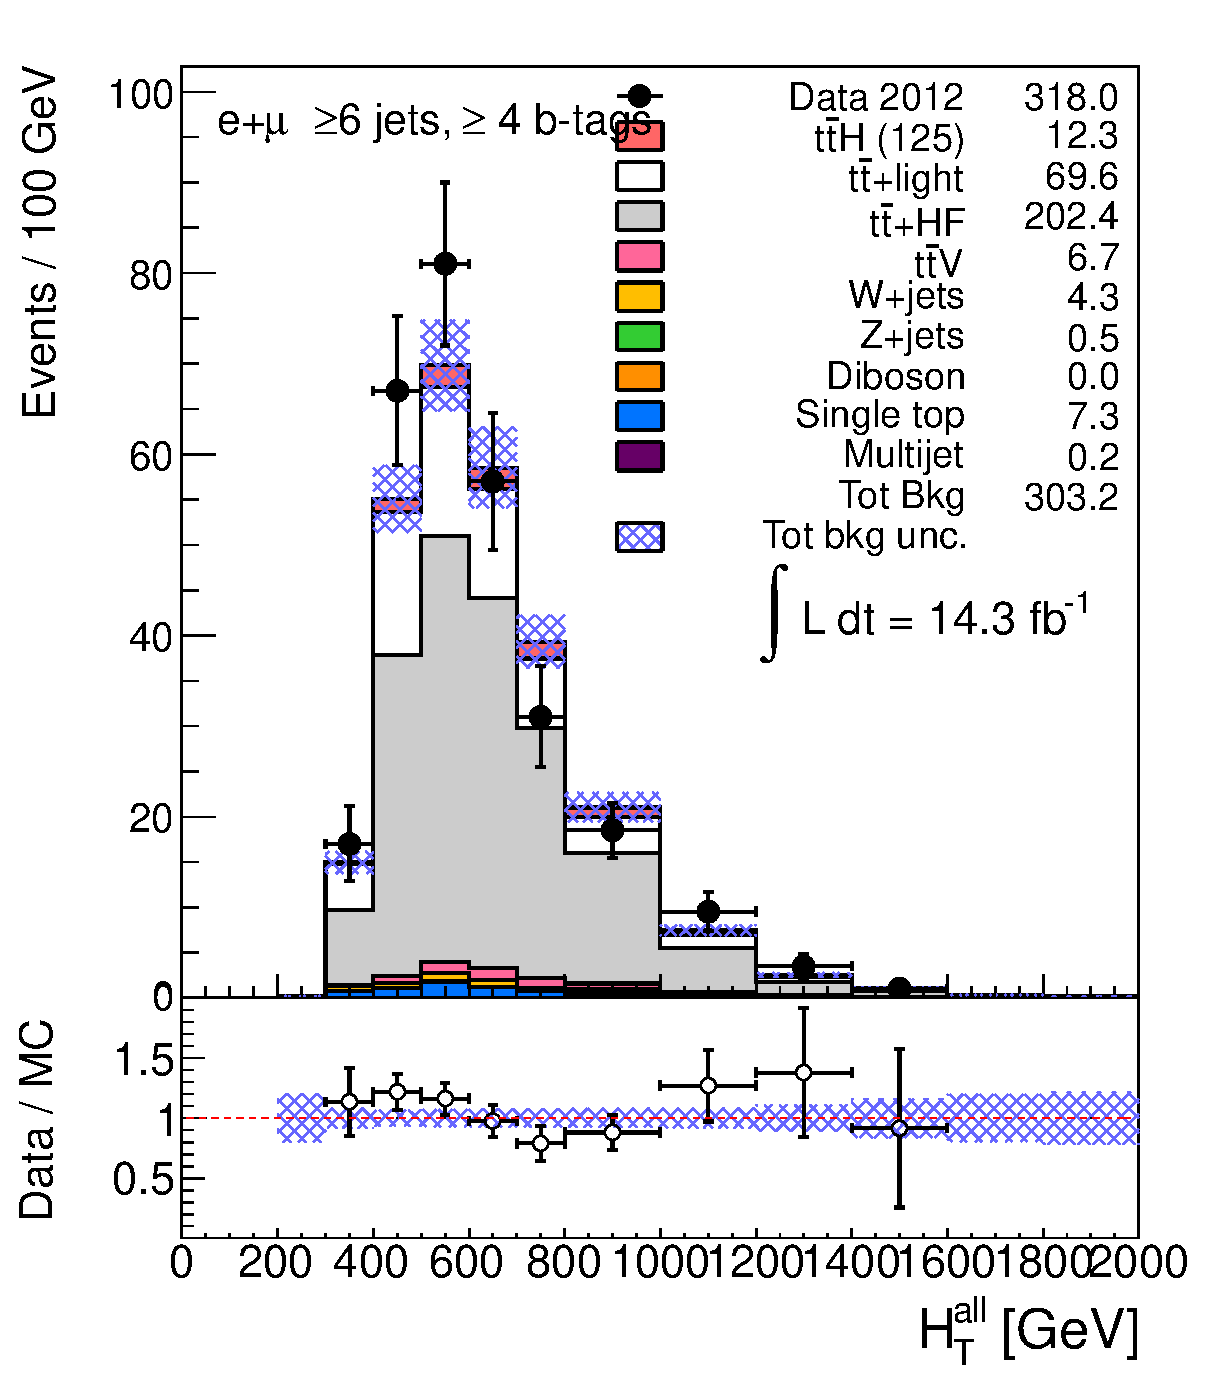
\includegraphics[width=0.27\textwidth]{htx_analysis_14ifb/figures/fullprof/PostFit_null/HTAll_6jetin4btagin_ELEMUON.eps}}
	\subfigure[]{
\includegraphics[width=0.27\textwidth]{htx_analysis_14ifb/figures/fullprof/sysband_Postfit_null/HTAll_6jetin4btagin_ELEMUON.eps}} \\
\caption{
Comparison between data and simulation for $\HT$ in the combined
electron and muon channels with $\geq 6$ jets and (a-c) \chii, (d-f) \chiii, and (g-i) \chiv.
From left to right: prefit (nominal $t\bar{t}$ \texttt{ALPGEN} prediction), 
postfit (full profiling of systematic uncertainties) and postfit (two-parameter fit).
The last bin in all figures contains the overflow. The bottom panel displays the ratio between data
and background prediction. The shaded area represents the total post-fit background uncertainty.}
%{\bf Caveat: for the "two-parameter fit" uncertainties are actually still prefit.}}
\label{fig:HT_SignalRegion_FullProfiling}
\end{center}\end{figure}



\section{Results}\label{sec:htxRES}

In the \htx\ analysis no significant excess of data over the 
expected background has been observed in the signal enriched 
\chiv\ channel of Figure~\ref{fig:htall4}.
The observed and expected upper limits on the \TTbar\ production cross section 
times branching fraction as a function of $m_{\T}$ are shown in 
Figure~\ref{fig:limits1D_htx} for the two chosen benchmark scenarios,
namely the weak-isospin singlet and
doublet models are chosen.
These results include both statistical and systematic uncertainties,
and the consistency of the data with the background prediction is 
assessed following the concepts presented in Section~\ref{sec:cls}
by computing the $p$-value under the background-only hypothesis
(1-$CL_{\rm b}$) for each point of the two-dimensional plane 
(each point corresponding to a signal scenario) and for every heavy 
quark mass point considered (one two-dimensional plane is built for each
$m_T$ value). For a vector-like $\T$ quark from a weak-isospin doublet, an observed (expected) 95\%  CL  limit
$m_{T}>790\,(745)\gev$ is obtained for the central value of the 
theoretical cross section.
For a vector-like singlet $\T$ quark, an observed (expected) 95\%  CL  limit 
$m_{\T}>640\,(615)\gev$ is obtained for the central value of the 
theoretical cross section.
%It has been verified that the expected signal yield and shape 
%of the $\HT$ distribution used to obtain the result in the doublet scenario is not
%significantly affected by the fact that signal MC samples corresponding to the singlet scenario were used (see Section~\ref{sec:SingletvsDoublet}).


Concerning the quasi-model independent strategy illustrated in Section~\ref{sec:strategy}, 
we recall here that a the two-dimensional plane was defined in order
to perform a scan of the allowed BRs.
To probe the full plane the signal samples are reweighted by the ratio
of desired branching ratio to the original branching ratio generated
by \texttt{PROTOS} and the complete analysis are repeated in each point.
The  95\% CL exclusion limits  obtained in the scan of the two-dimensional
plane by varying the mixing of the three decay channel contributions for
different values of $m_{\T}$ are shown in Figure~\ref{fig:limits2D_wbx}. 
This plot reads as follow: taking for instance the $600\gev$ 
vector-like top partner, a heavy quark with
$BR(\T\to Ht)>0.3$ is excluded at $\geq 95\%$ CL,
regardless of the value of the vector-like quark branching ratios to $Wb$ and $Zt$.  
It was also attempted to perform the \htx\ analysis
using \B\ quark samples as signals, but the results
have not been satisfactory enough as can be seen in the
BR plane of Figure~\ref{fig:limits2D_htxvlb}.
%A comparison of expected limits for different configurations on the number of channels considered and
%profiled parameters is presented in App.~\ref{sec:expected_limits_Appendix}. 


%%%%%%%%%%%%%%
\begin{figure}[htbp]
\begin{center}
\begin{tabular}{cc}
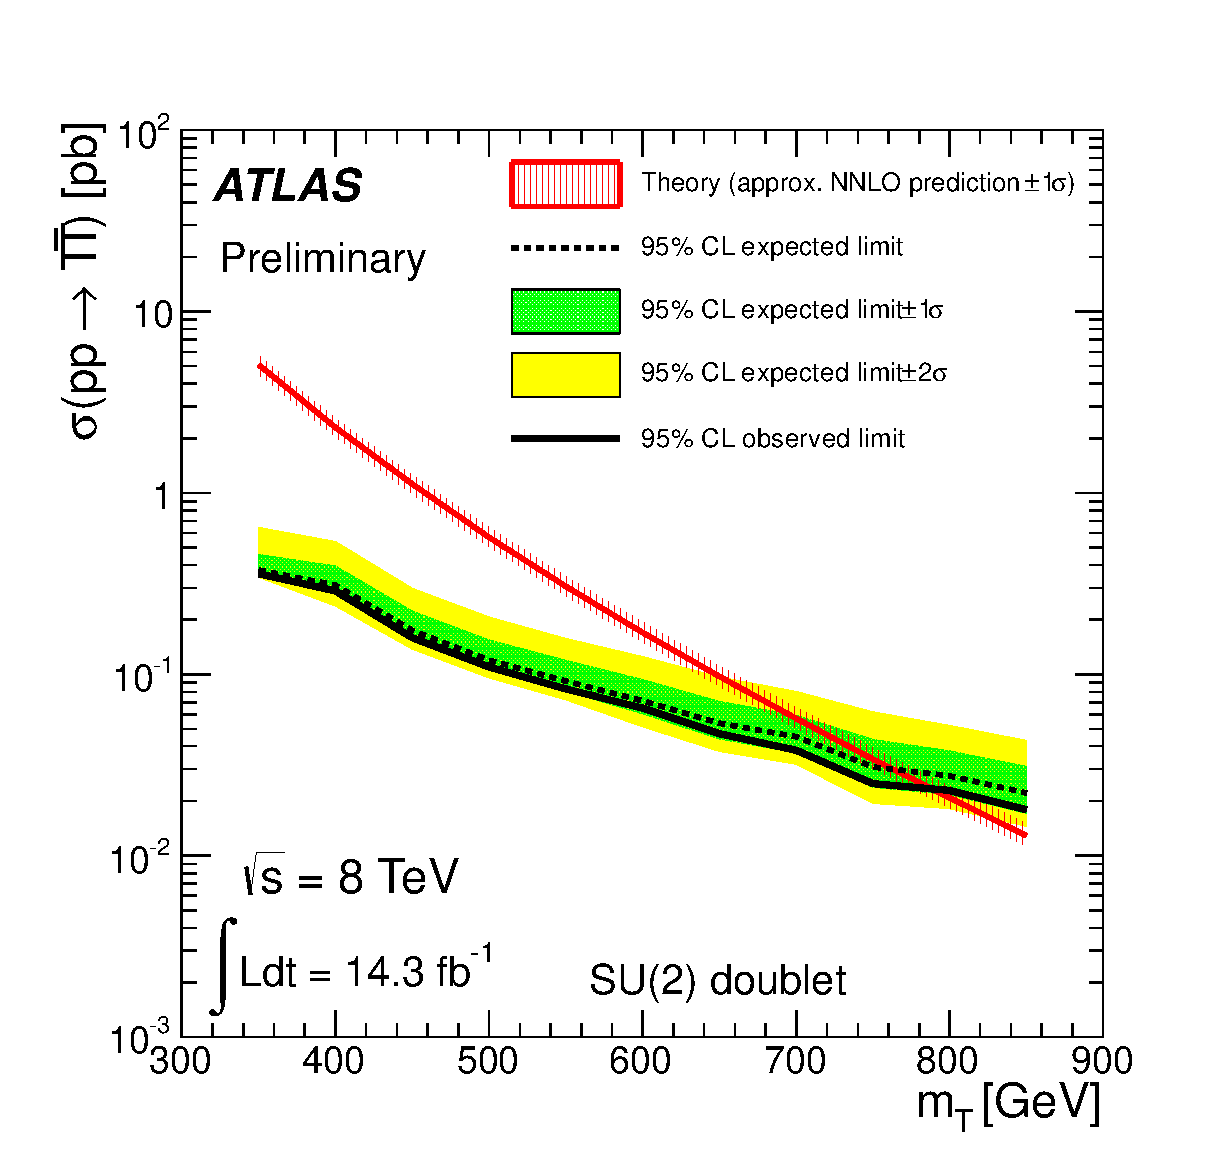
\includegraphics[width=0.45\textwidth]{results/figures/htx/lim_doublet.eps} &
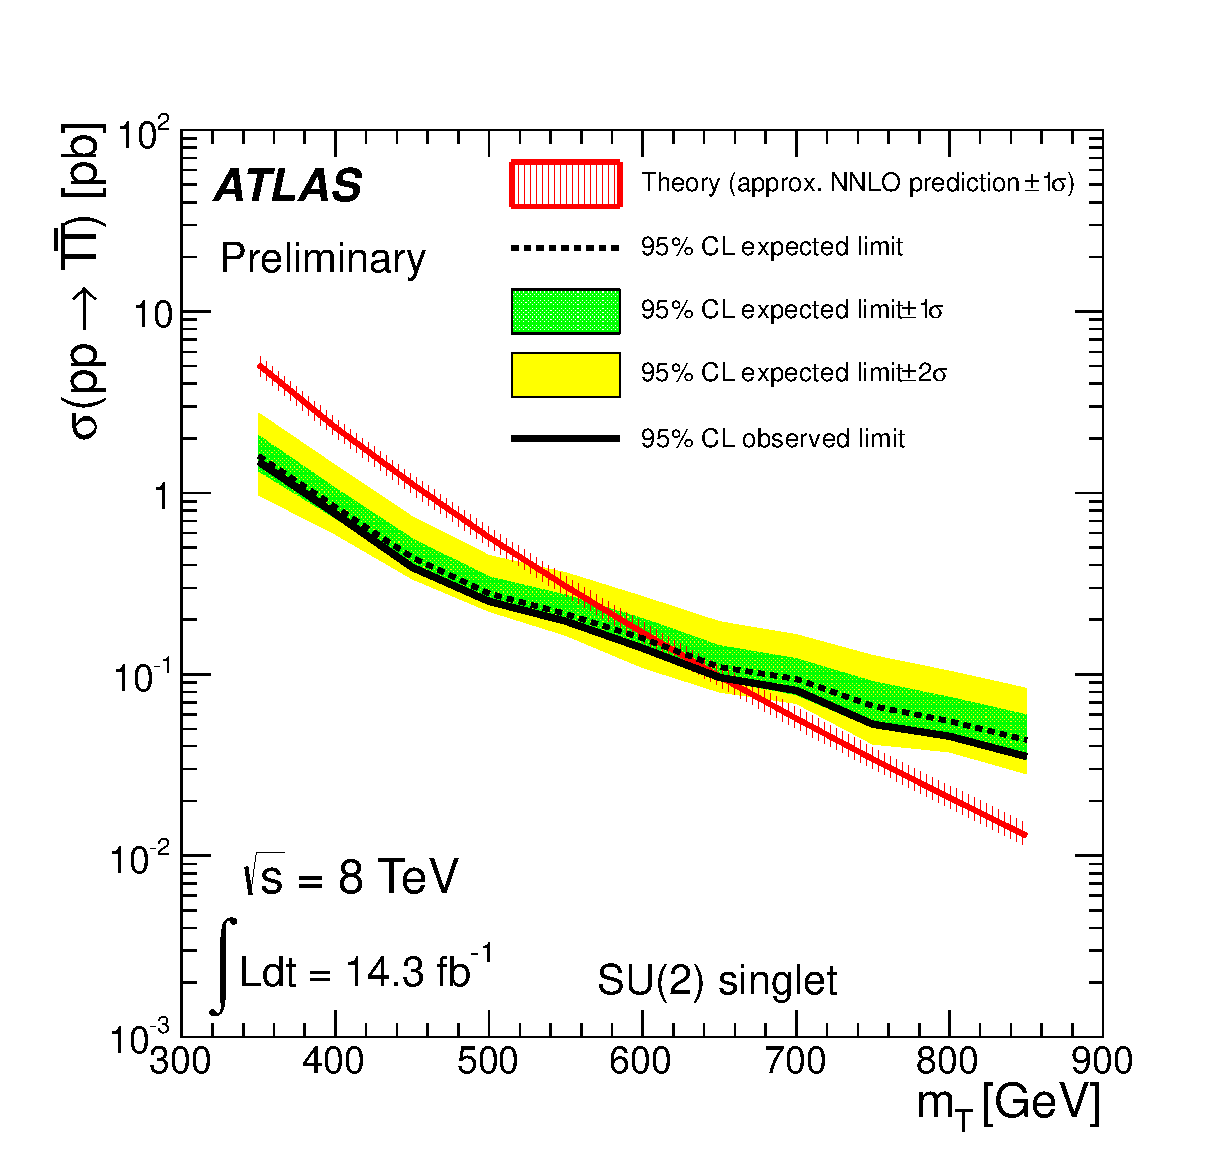
\includegraphics[width=0.45\textwidth]{results/figures/htx/lim_singlet.eps} \\
(a) & (b) \\
\end{tabular}
\caption{Observed (solid line) and expected (dashed line) 95\% CL upper limits on the $t^\prime \bar{t^\prime}$ cross section times branching fraction
for a weak-isospin (a) doublet and (b) singlet $\T$ quark  as a function of the $\T$ quark mass. 
\label{fig:limits1D_htx}}
\end{center}
\end{figure}

\begin{figure}[htbp]
\centering
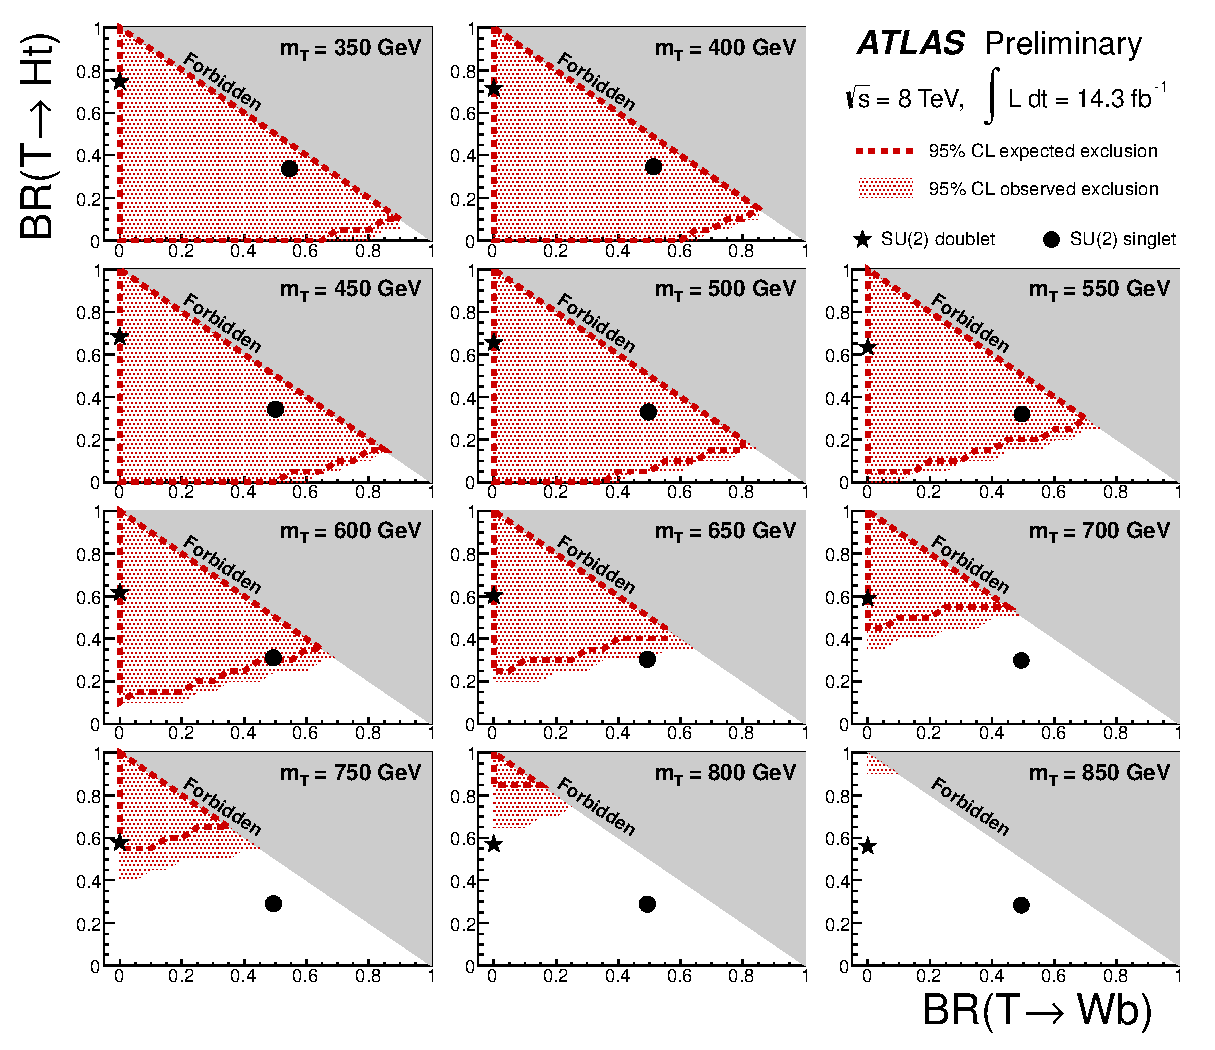
\includegraphics[width=0.9\textwidth]{results/figures/htx/lim_2D.eps}
\caption{
Observed (red filled area) and expected (red dashed line) 95\% CL exclusion in the plane of
$BR(\T \to Wb)$ versus $BR(\T \to Ht)$, for different values of the vector-like $\T$ quark mass.
\label{fig:limits2D_htx}}
\end{figure}
%%%%%%%%%%%%%%


\begin{figure}[htb]\begin{center}
	\subfigure{
  	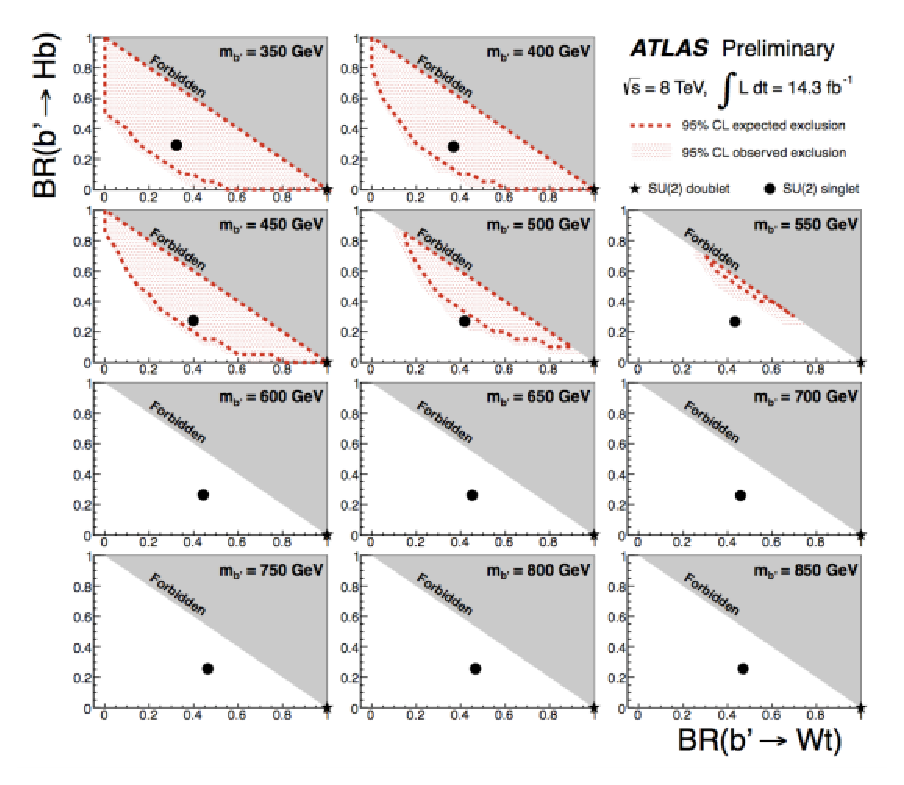
\includegraphics[width=0.9\textwidth]{htx_analysis_14ifb/figures/vlbBRplane.eps}}
	\caption{Observed (red filled area) and expected (red dashed line) 95\% CL exclusion in the plane of
        $BR(\B \to Wt)$ versus $BR(\B \to Hb)$, for different values of the vector-like $\B$ quark mass.
        \label{fig:limits2D_htxvlb}}
\end{center}\end{figure}

\section{Outlook}\label{sec:htxOUT}

It has been shown that for the \htx\ analysis one evident issue
is the poor modeling of the
heavy-flavor component of the main Standard Model background, the
\ttbar+jets background.
Since this comes from the Monte Carlo generators parameters, 
studies are needed to identify the corrections to this problem.
Another issue regards the calibration of \btag ged jets,
which needs to be improved for analyses such this involving
high \bjet s multiplicities.

As explained in Section~\ref{sec:fullprof}, 
the sensitivity of the search can gain much from an
eventual full profiling of the nuisance parameters, thanks to the
background-enriched sidebands in the three final search channels.
Finally, the \htx\ analysis strategy can be easily
extended, with minor modification, to searches for $B\to Hb+X$.
A possible addition to the search strategy is attempting
the reconstruction of the Higgs boson from, eventually,
boosted \bjet s, somehow similarly to what is done in the
\wbx\ analysis.

